\documentclass{article}

\usepackage{amsmath,geometry,amsfonts,array,makecell,enumitem,bm,esint,booktabs,multirow,mathtools,pgfplots,amssymb}
\usepackage[amsmath]{ntheorem}
\usepackage[hidelinks]{hyperref}
\usepackage[nameinlink,noabbrev]{cleveref}
\usepackage{ragged2e}
\usepackage{fancyhdr}
\pagestyle{fancy}
\fancyhead[L]{\itshape\nouppercase{\leftmark}}
\fancyhead[R]{IB Complex Analysis}

\title{Complex Analysis}
\author{Yue Wu}

\geometry{a4paper,hmargin=1.1in,vmargin=1.2in}

\setlength{\parskip}{1em}
\tolerance=1000
\emergencystretch=1em
\hyphenpenalty=1000
\exhyphenpenalty=100
\righthyphenmin=3

\theoremstyle{plain}\theoremheaderfont{\normalfont\itshape}\theorembodyfont{\rmfamily}\theoremseparator{.}\newtheorem*{rem}{Remark}\newtheorem*{ex}{Example}\newtheorem*{proof}{Proof}\newtheorem*{altp}{Alternative proof}\newtheorem*{con}{Consequences}\newtheorem*{notn}{Notations}\newtheorem*{cau}{Caution}\newtheorem*{term}{Terminology}\newtheorem*{keyex}{Key example}

\theoremstyle{plain}\theoremheaderfont{\normalfont\bfseries}\theorembodyfont{\rmfamily}\theoremseparator{.}\newtheorem{thm}{Theorem}[section]\newtheorem{lem}[thm]{Lemma}\newtheorem{prop}[thm]{Proposition}\newtheorem*{cor}{Corollary}\newtheorem{defn}[thm]{Definition}\newtheorem{clm}[thm]{Claim}\newtheorem{clminproof}{Claim}\newtheorem{leminproof}{Lemma}\newtheorem{app}{Application}

\theoremstyle{break}\theoremheaderfont{\normalfont\itshape}\theorembodyfont{\rmfamily}\theoremseparator{.\medskip}\newtheorem*{proofskip}{Proof}\newtheorem*{exs}{Examples}\newtheorem*{rems}{Remarks}\newtheorem*{rec}{Recall}\newtheorem*{ppts}{Properties}

\theoremstyle{break}\theoremheaderfont{\normalfont\bfseries}\theorembodyfont{\rmfamily}\theoremseparator{.\medskip}\newtheorem{lemskip}[thm]{Lemma}\newtheorem{defnskip}[thm]{Definition}\newtheorem{propskip}[thm]{Proposition}\newtheorem{thmskip}[thm]{Theorem}

\crefname{thm}{Theorem}{Theorems}\crefname{defn}{Definition}{Definitions}\crefname{lem}{Lemma}{Lemmas}\crefname{lemskip}{Lemma}{Lemmas}\crefname{cor}{Corollary}{Corollaries} \crefname{prop}{Proposition}{Propositions}\crefname{clm}{Claim}{Claims}

\numberwithin{equation}{section}
\setcounter{tocdepth}{2}

\usetikzlibrary{decorations.markings}

\newlength\ubwidth
\newcommand\parunderbrace[2]{\settowidth\ubwidth{$#1$}\underbrace{#1}_{\parbox{\ubwidth}{\scriptsize\RaggedRight#2}}}

\newcommand{\ii}{\mathrm{i}}
\newcommand{\ee}{\mathrm{e}}
\DeclareMathOperator*{\Arg}{Arg}
\DeclareMathOperator*{\Log}{Log}
\DeclareMathOperator*{\Res}{Res}
\DeclareMathOperator*{\length}{length}
\DeclareMathOperator*{\Deg}{Deg}
\DeclareMathOperator*{\inter}{int}
\newcommand{\qed}{\hfill\ensuremath{\Box}}
\newcommand{\abs}[1]{\left|#1\right|}
\newcommand{\norm}[1]{\left\|#1\right\|}
\newcommand{\dd}[2][]{\,\mathrm{d}^{#1} #2}
\newcommand{\NN}{\mathbb{N}}
\newcommand{\ZZ}{\mathbb{Z}}
\newcommand{\QQ}{\mathbb{Q}}
\newcommand{\RR}{\mathbb{R}}
\newcommand{\CC}{\mathbb{C}}
\newcommand{\HH}{\mathbb{H}}
\newcommand{\DD}{\mathbb{D}}
\newcommand{\dv}[2]{\frac{\mathrm{d}#1}{\mathrm{d}#2}}
\renewcommand{\Re}{\operatorname{Re}}
\renewcommand{\Im}{\operatorname{Im}}

\pgfplotsset{compat=1.18}


\begin{document}
    \setlength{\parindent}{0pt}
	\Huge\textsf{\textbf{Complex Analysis}}
		
	\Large\textsf{\textbf{University of Cambridge Part IB Mathematical Tripos}}

	\noindent\makebox[\linewidth]{\rule{\textwidth}{2pt}}

	\large\textsf{\textbf{Yue Wu}}
	\begin{itemize}[topsep=0pt,leftmargin=15pt]
		\item[] \textit{Yusuf Hamied Department of Chemistry\\
		Lensfield Road,\\
		Cambridge, CB2 1EW}\\

		\textit{yw628@cam.ac.uk}
	\end{itemize}
    \thispagestyle{empty}
    \pagenumbering{roman}
    \setlength{\parindent}{15pt}
	
    \normalsize
    \newpage
	\tableofcontents
	\newpage
    \pagenumbering{arabic}

    \section{Introduction}
    The goal of this course: study the theory of complex-valued differentiable functions in one complex variable.
    \begin{enumerate}[topsep=0pt,label=(\roman*)]
        \item Polynomial
        \[ p(z)=a_dz^d+\dots+a_1z^1+a_0\,, \]
        coefficients in \(\ZZ\), \(\QQ\), \(\RR\) and \(\CC\). \hfill \(\Rightarrow\) algebraic geometry
        \item Series
        \[ \sum_{n=1}^{\infty}\frac{1}{n^s} \]
        \(\CC\) is the right place to study. \hfill \(\Rightarrow\) number theory
        \item Harmonic functions
        \begin{align*}
            u(x,y):\RR^2&\to\RR\\
            u_{xx}+u_{yy}&=0
        \end{align*}
        \hfill\(\Rightarrow\) PDE
        \item Real integrals via complex integrals.
    \end{enumerate}
    \begin{notn}
        For \(z\in\CC\), \(z=x+\ii y\), where \(x,y\in\RR\).
        \begin{itemize}[topsep=0pt]
            \item \(x=\Re z\) is the real part, \(y=\Im z\) is the imaginary part.
            \item \(\bar{z}=x-\ii y\) is the complex conjugate.
            \item \(\abs{z}=\sqrt{x^2+y^2}\) is the modulus and \(\arg(z)\) is the argument. If we choose \(\theta\in(-\pi,\pi)\), then this is the principal argument \(\Arg(z)\).
            \item \(\CC^*\coloneqq\CC\setminus\{0\}\), \(\CC_\infty\coloneqq\CC\cup\{\infty\}\).
            \item \( D(a,r)\coloneqq\{z\in\mathbb{C}\mid\abs{z-a}<r\}\) is an open disk of radius \(r\) centred at \(a\). \(\DD\coloneqq D(0,1)\) is the unit disk at the origin.
        \end{itemize}
    \end{notn}

    \begin{defnskip}
        \begin{enumerate}[topsep=0pt,label=(\roman*)]
            \item \(U\subseteq\CC\) is \textit{open} if \(\forall u\in U\), \(\exists\epsilon>0\) such that
            \[ D(u,\epsilon)=\{z\in\mathbb{C}\mid\abs{z-u}<\epsilon\}\subseteq U\,. \]
            \item A \textit{path} in \(U\subset\CC\) is a continuous map \(\gamma:[a,b]\to U\). We say \(\gamma\in C^1\) if \(\gamma'\) exists and is continuous (one-sided at end-points).
            \item A path \(\gamma\) is \textit{simple} if \(\gamma\) is injective.
            \item \(U\subseteq\CC\) is \textit{path-connected} if \(\forall z,w\in U\), \(\exists\) path in \(U\) connecting \(z\) to \(w\).
        \end{enumerate}
    \end{defnskip}
    \begin{rem}
        If \(U\) is open and \(z,w\) are connected by a path \(\gamma\) in \(U\), then \(\exists\) a path \(P\) in \(U\) consisting of finitely many horizontal and vertical segments.
    \end{rem}

    \newpage
    \section{Complex Differentiation}
    \begin{defn}
        A \textit{domain} in \(\CC\) is an open, path-connected, non-empty subset of \(\CC\). 
    \end{defn}
    \begin{defnskip}
        \begin{enumerate}[topsep=0pt,label=(\roman*)]
            \item \(f:U\to\mathbb{C}\) on a domain \(U\) is \textit{differentiable} at \(u\in U\) if
            \[ f'(u)=\lim_{z\to u}\frac{f(z)-f(u)}{z-u} \]
            exists.
            \item \(f:U\to\mathbb{C}\) is \textit{holomorphic} at \(u\in U\) if \(\exists\epsilon>0\) such that \(\forall z\in D(u,\epsilon)\), \(f\) is differentiable at \(z\).
            \item \(f:\CC\to\CC\) is \textit{entire} if it is holomorphic on \(\CC\).
        \end{enumerate}
    \end{defnskip}
    We may identify \(\CC\) with \(\RR^2\) via the bijection
    \[ x+\ii y\leftrightarrow(x,y)\,. \]
    Then what is the connection with \(\mathbb{R}^2\) differentiability?
    \begin{rem}
        All computational differentiation rules still hold for holomorphic functions: sum, product, quotient, chain, inverse\dots
    \end{rem}

    If we have complex-valued function \(f:U\to\mathbb{C}\), then we can write
    \[ f(z)=f(x,y)=u(x,y)+\ii v(x,y)\, \]
    where \(u\) is the real part and \(v\) is the imaginary part. From Analysis and Topology, \(u:U\to\mathbb{R}\) is differentiable at \((c,d)\in\mathbb{R}^2\) with \(\left.Du\right|_{(c,d)}=(\lambda,\mu)\) if
    \[ \frac{u(x,y)-u(c,d)-[\lambda(x-c)+\mu(y-d)]}{\sqrt{(x-c)^2+(y-d)^2}}\to 0 \]
    as \((x,y)\to(c,d)\).

    \begin{prop}[Cauchy--Riemann Equations]
        Let \(f:U\to\mathbb{C}\) on an open set \(U\subseteq\CC\), then \(f\) is differentiable at \(w=c+\ii d\in U\) with \(f'(w)=p+\ii q\) if and only if, writing \(f=u+\ii v\), we have \(u,v\) are real differentiable at \((c,d)\) and
        \[\left\{\begin{aligned}
            u_x&=v_y\\
            -u_y&=v_x\,,
        \end{aligned}\right.\]
        known as the \textit{Cauchy--Riemann equations}.
    \end{prop}
    \begin{proof}
		\(f\) is differentiable at \(w=c+\ii d\) with \(f'(w)=p+\ii q\)
		\begin{align*}
			&\iff\quad\lim_{z\to w}\frac{f(z)-f(w)-(z-w)(p+\ii q)}{z-w}=0\\
			&\iff\quad\lim_{z\to w}\frac{f(z)-f(w)-(z-w)(p+\ii q)}{\abs{z-w}}=0\,.
		\end{align*}
		Writing \(f=u+\ii v\) and evaluating the real and imaginary parts, this holds
        \[\iff\quad\left\{\begin{aligned}
            &\lim_{(x,y)\to(c,d)}\frac{u(x,y)-u(c,d)-[p(x-c)-q(y-d)]}{\sqrt{(x-c)^2+(y-d)^2}}=0\\
            &\lim_{(x,y)\to(c,d)}\frac{v(x,y)-v(c,d)-[q(x-c)+p(y-d)]}{\sqrt{(x-c)^2+(y-d)^2}}=0\,.
        \end{aligned}\right.\]
		These hold iff \(u,v\) are real differentiable and \(u_x=p=v_y\), \(u_y=-q=-v_x\).\qed
	\end{proof}
    \begin{rem}
        If \(u,v\) have continuous partials \(u_x,u_y,v_x,v_y\) on \(U\), then \(u\) and \(v\) are differentiable on \(U\). So for complex differentiability of \(f=u+\ii v\), it suffices to check \(u,v\) have continuous partials on \(U\) and the Cauchy--Riemann equations hold.
    \end{rem}
    \textit{Examples.}
    \begin{enumerate}[topsep=0pt,label=(\roman*)]
        \item \(f(z)=z^2=(x+\ii y)^2=\underbrace{x^2-y^2}_{u}+\underbrace{2xy}_{v}\ii\).
        \[u_x=v_y=2x\,,\; u_y=-v_x=-2y\,,\]
        so \(f\) is entire and \(f'(z)=2x+2\ii y=2z\).
        \item \(f(z)=\bar{z}\).
        \[u(x,y)=x\,,\;v(x,y)=-y\,,\]
        so \(f\) is not holomorphic anywhere.
        \item Any polynomial is entire, and any rational map
        \[f(z)=\frac{p(z)}{q(z)}\,,\]
        where \(p\) and \(q\) are polynomials, is holomorphic on \(\{z\in\mathbb{C}\mid q(z)\ne 0\}\).
    \end{enumerate}
    \begin{cau}
        Satisfying Cauchy--Riemann equations is not sufficient alone for complex differentiability.
    \end{cau}
    \begin{rem}
        If \(f:U\to\mathbb{C}\) holomorphic on a domain \(U\), and \(f'(z)=0\) on \(U\), then \(f\) is constant on \(U\).

        Sketch of proof: take a \(z_0\in U\) and connect for \(z\in U\) by a vertical/horizontal path and use the partials. 
    \end{rem}
    \begin{con}
        Holomorphic functions are very ``well-behaved''.
        \begin{enumerate}[topsep=0pt,label=(\roman*)]
            \item {[Structural]} \textit{Example} (proved later). If \(f:\CC\to\CC\) is entire and bounded, i.e. \(\exists M\ge 0\) such that \(\abs{f(z)}\le M\; \forall z\in\CC\), then \(f\) is constant.
            
            In contrast with real differentiable functions \((x,y)\mapsto(\cos x,\sin y)\).
            \item {[Analyticity]} We will see if \(f\) is holomorphic, then all derivatives of \(f\) (and of \(u,v\), where \(f=u+\ii v\)) exist.
            
            Differentiating Cauchy--Riemann equations, we obtain
            \[u_{xx}=v_{yx}=v_{xy}=-u_{yy}\,,\]
            so
            \[u_{xx}+u_{yy}=0\,,\]
            and similarly \(v_{xx}+v_{yy}=0\), The real and imaginary parts of a holomorphic function are harmonic.
        \end{enumerate}
    \end{con}
    
    \subsection{The Geometry of Harmonic Functions}
    \begin{prop}
        \(U\) is a domain, \(w\in U\) and \(f:U\to\mathbb{C}\) holomorphic with \(f'(w)\ne 0\). Then \(f\) is \textit{conformal} (angle preserving) at \(w\).
    \end{prop}
    \begin{figure}[ht!]
        \centering
        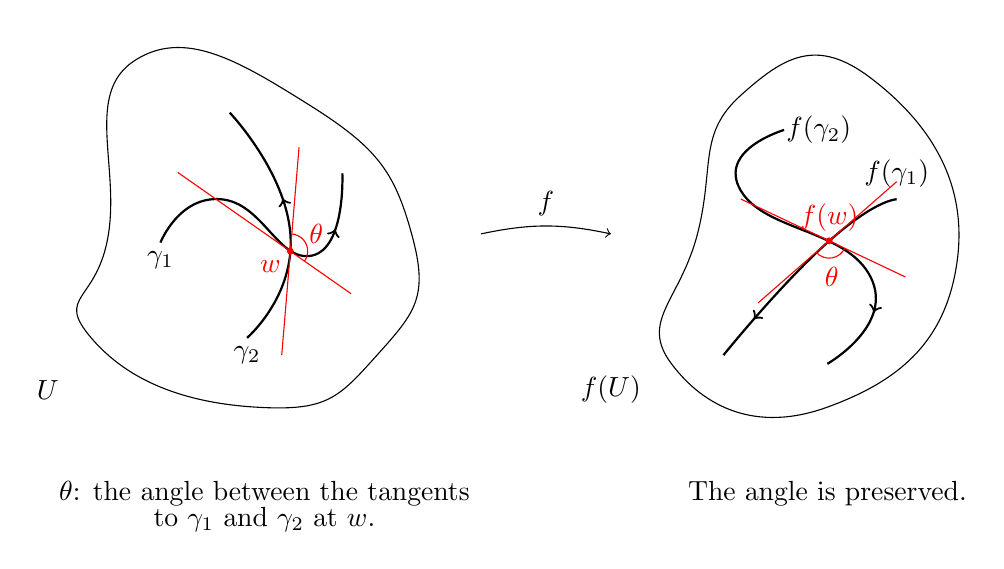
\begin{tikzpicture}[scale=1.1]
            \draw plot[smooth cycle,tension = 0.9] coordinates {(-0.3,0) (0,2) (2,1.5) (3.2,0) (2.8,-1.4) (1.4,-2) (-0.5,-1.2)};
            \node at (-1,-1.8) {\(U\)};
            \draw[decoration={markings, mark=at position 0.6 with {\arrow{>}}},postaction={decorate},thick] plot[smooth, tension=1] coordinates {(1.3,-1.2) (1.8,0) (1.1,1.4)}; 
            \node at (1.3,-1.4) {\(\gamma_2\)};
            \draw[decoration={markings, mark=at position 0.8 with {\arrow{>}}},postaction={decorate},thick] plot[smooth, tension=1] coordinates {(0.3,-0.1) (1,0.4) (2.05,-0.25) (2.4,0.7)};
            \node at (0.3,-0.3) {\(\gamma_1\)};
            \fill[red] (1.8,-0.2) circle (0.04) node[below left]{\(w\)};
            \draw[red] (0.5,0.71)--(2.5,-0.69);
            \draw[red] (1.9,1)--(1.7,-1.4);
            \draw[red] (1.817,-0.001) arc (85.24:-35:0.2);
            \node[red] at (2.1,0) {\(\theta\)};

            \node at (1.5,-3) {\(\theta\): the angle between the tangents};
            \node at (1.5,-3.3) {to \(\gamma_1\) and \(\gamma_2\) at \(w\).};

            \draw[->] (4,0) to [bend left=12] node[above]{\(f\)}(5.5,0);

            \draw plot[smooth cycle,tension = 0.9] coordinates {(6.5,0) (7,1.6) (8.5,1.8) (9.5,-0.3) (8,-2) (6.2,-1.5)};
            \node at (5.5,-1.8) {\(f(U)\)};
            \draw[decoration={markings, mark=at position 0.8 with {\arrow{>}}},postaction={decorate},thick] plot[smooth, tension=1] coordinates {(7.5,1.2) (7,0.5) (8.5,-0.5) (8,-1.5)};
            \node at (7.9,1.2) {\(f(\gamma_2)\)};
            \draw[decoration={markings, mark=at position 0.8 with {\arrow{>}}},postaction={decorate},thick] plot[smooth, tension=1] coordinates {(8.8,0.4) (8,-0.1) (6.8,-1.4)};
            \node at (8.8,0.7) {\(f(\gamma_1)\)};
            \fill[red] (8.02,-0.08) circle (0.04) node[above]{\(f(w)\)};
            \draw[red] (7,0.403)--(8.9,-0.497);
            \draw[red] (8.8,0.603)--(7.2,-0.797);
            \draw[red] (7.869,-0.2117) arc (221.2:334.65:0.2);
            \node[red] at (8.05,-0.5) {\(\theta\)};
            \node at (8,-3) {The angle is preserved.};
        \end{tikzpicture}
    \end{figure}
    \begin{proof}
        Let \(\gamma_1\) and \(\gamma_2\) be \(C^1\) paths through \(w\in U\) with \(\gamma_1,\gamma_2\) defined on \([-1,1]\) with \(\gamma_1(0)=\gamma_2(0)=w\). Write \(\gamma_j(t)=w+r_j(t)\ee^{\ii \theta_j(t)}\). We have
        \[\theta=\Arg(\gamma_2'(0))-\Arg(\gamma_1'(0))=\theta_2(0)-\theta_1(0)\,.\]
        Since \(f'(w)\ne 0\),
        \begin{align*}
            \Arg((f\circ\gamma_j)'(0))&=\Arg(\gamma_j'(0)f'(\gamma_j(0)))\\
            &=\Arg(\gamma_j'(0))+\Arg(f'(w))+2n\pi\,,\;n\in\ZZ\,.
        \end{align*}
        So the angle between the image \(f\circ\gamma\) paths at \(w\) is
        \[\Arg(\gamma_2'(0))+\Arg(f'(w))+2n_2\pi-\Arg(\gamma_1'(0))-\Arg(f'(w))-2n_1\pi\,,\]
        so the angle is preserved.\qed
    \end{proof}
    \begin{defn}
        \(U\), \(V\) are domains in \(\CC\). A map \(f:U\to V\) is a \textit{conformal equivalence} if \(f\) is a bijective holomorphic map with \(f'(z)\ne 0\) \(\forall z\in U\). We say \(U\) and \(V\) are \textit{conformally equivalent} if such map exists.
    \end{defn}
    \begin{rems}
        \begin{enumerate}[topsep=0pt,label=(\roman*)]
            \item One can show that if \(f:U\to V\) is a holomorphic bijection of domains with \(f'(z)\ne 0\) \(\forall z\in U\), then the inverse of \(f\) is holomorphic.
            \item We will see that if \(f\) is an injection and is holomorphic in \(U\), then \(f'\ne 0\) on \(U\).
        \end{enumerate}
    \end{rems}
    \begin{exs}
        \begin{enumerate}[topsep=0pt,label=(\roman*),parsep=1em]
            \item Change of coordinates:
            
            On \(\mathbb{C}\), \(f(z)=az+b\), \(a\ne 0\) is a conformal equivalence \(\mathbb{C}\to\mathbb{C}\). More generally, the M\"{o}bius transformation
            \[f(z)=\frac{az+b}{cz+d}\,,\; ad\ne cb\]
            is a conformal equivalence \(\CC_\infty\xrightarrow{\sim}\CC_\infty\) the Riemann sphere to itself.
            \begin{itemize}
                \item Conformality/holomorphicity at infinity: use pre/post composition by M\"{o}bius maps to move away from \(\infty\) then test conformality/holomorphicity.
                \begin{rem}
                    Differentiability is independent of the choice of coordinates, but the values of derivatives are not.
                \end{rem}
                \item Features of M\"{o}bius maps:
                \begin{enumerate}
                    \item Determined by 3 distinct points.
                    \[\begin{cases}
                        z_1\mapsto 0\\
                        z_2\mapsto \infty\\
                        z_3\mapsto 1
                    \end{cases}\quad\implies\mu(z)=\frac{z-z_1}{z-z_2}\cdot\frac{z_3-z_2}{z_3-z_1}\,.\]
                    \item it maps lines/circles to lines/circles.
                \end{enumerate}
            \end{itemize}
            \item \(f(z)=z^n\), \(n\in\NN\) on a sector \(\{z\in\mathbb{C}^*\mid 0<\Arg(z)<\frac{\pi}{n}\}\).
            \begin{figure}[ht!]
                \centering
                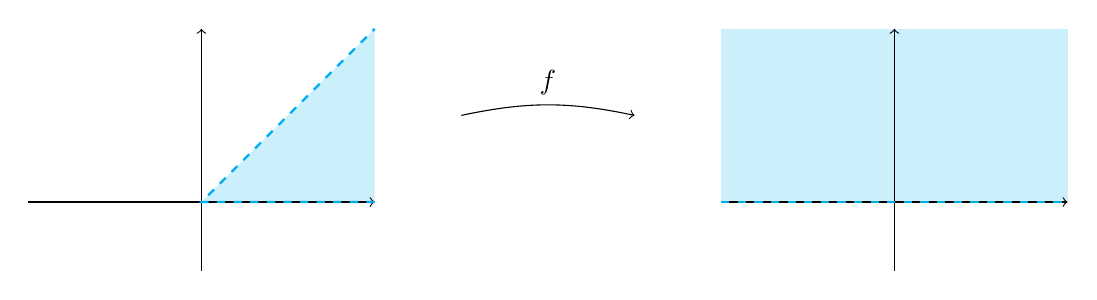
\begin{tikzpicture}[scale=1.1]
                    \fill[cyan!20] (2,0)--(0,0)--(2,2);
                    \draw[->] (-2,0)--(2,0);
                    \draw[->] (0,-0.8)--(0,2);
                    \draw[thick,dashed,cyan] (2,0)--(0,0)--(2,2);
                    \draw[->] (3,1) to [bend left=12] node[above]{\(f\)}(5,1);
                    \fill [cyan!20] (6,0) rectangle (10,2);
                    \draw[->] (6,0)--(10,0);
                    \draw[->] (8,-0.8)--(8,2);
                    \draw[thick,dashed,cyan] (6,0)--(10,0);
                \end{tikzpicture}
            \end{figure}
            \item Upper half plane \(\HH\) and \(D(0,1)\) are conformally equivalent.
            \[g^{-1}(w)=-\ii\frac{w+1}{w-1}\,.\]
            \begin{figure}[ht!]
                \centering
                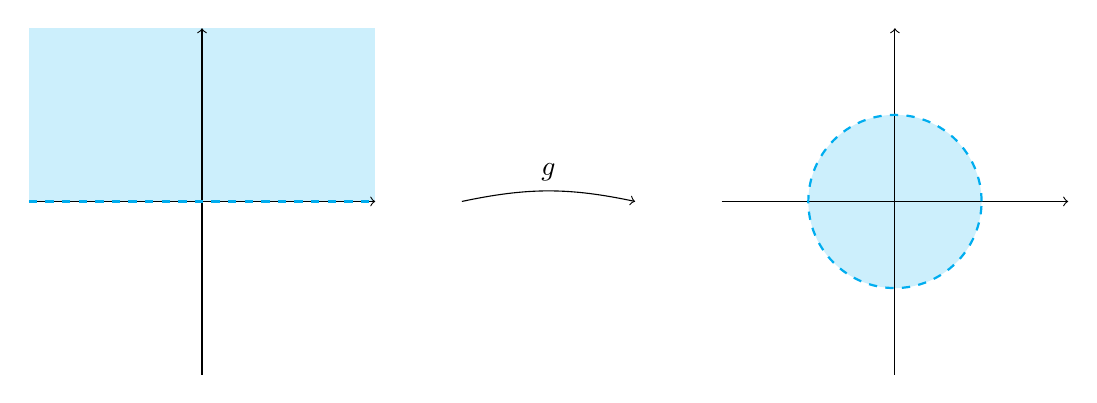
\begin{tikzpicture}[scale=1.1]
                    \fill [cyan!20] (-2,0) rectangle (2,2);
                    \draw[->] (-2,0)--(2,0);
                    \draw[->] (0,-2)--(0,2);
                    \draw [thick,dashed,cyan] (-2,0)--(2,0);
                    \draw[->] (3,0) to [bend left=12] node[above]{\(g\)}(5,0);
                    \fill[cyan!20] (8,0) circle (1);
                    \draw[->] (6,0)--(10,0);
                    \draw[->] (8,-2)--(8,2);
                    \draw [thick,dashed,cyan] (8,0) circle (1);
                \end{tikzpicture}
            \end{figure}
            \item A half circle and a half plane are conformally equivalent.
            \begin{figure}[ht!]
                \centering
                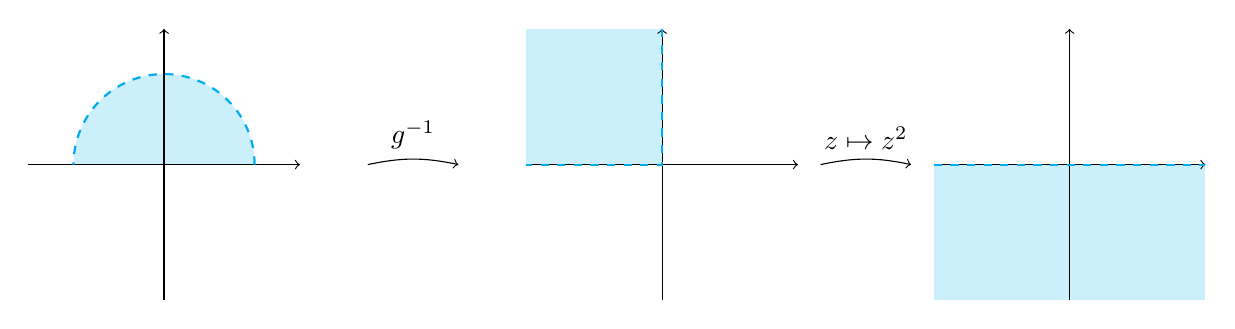
\begin{tikzpicture}[scale=1.15]
                    \fill[cyan!20] (1,0) arc (0:180:1);
                    \draw[->] (-1.5,0)--(1.5,0);
                    \draw[->] (0,-1.5)--(0,1.5);
                    \draw[thick,dashed,cyan] (1,0) arc (0:180:1);
                    \draw[->] (2.25,0) to [bend left=12] node[above]{\(g^{-1}\)}(3.25,0);
                    \fill[cyan!20] (4,0) rectangle (5.5,1.5);
                    \draw[->] (4,0)--(7,0);
                    \draw[->] (5.5,-1.5)--(5.5,1.5);
                    \draw[thick,dashed,cyan] (5.5,1.5)--(5.5,0)--(4,0);
                    \draw[->] (7.25,0) to [bend left=12] node[above]{\(z\mapsto z^2\)}(8.25,0);
                    \fill[cyan!20] (8.5,-1.5) rectangle (11.5,0);
                    \draw[->] (8.5,0)--(11.5,0);
                    \draw[->] (10,-1.5)--(10,1.5);
                    \draw[thick,dashed,cyan] (8.5,0)--(11.5,0);
                \end{tikzpicture}
            \end{figure}
            \item The possible images of a sector under a M\"{o}bius map.
            
            A sector is defined by lines intersecting at \(0\) and \(\infty\).
            \begin{figure}[ht!]
                \centering
                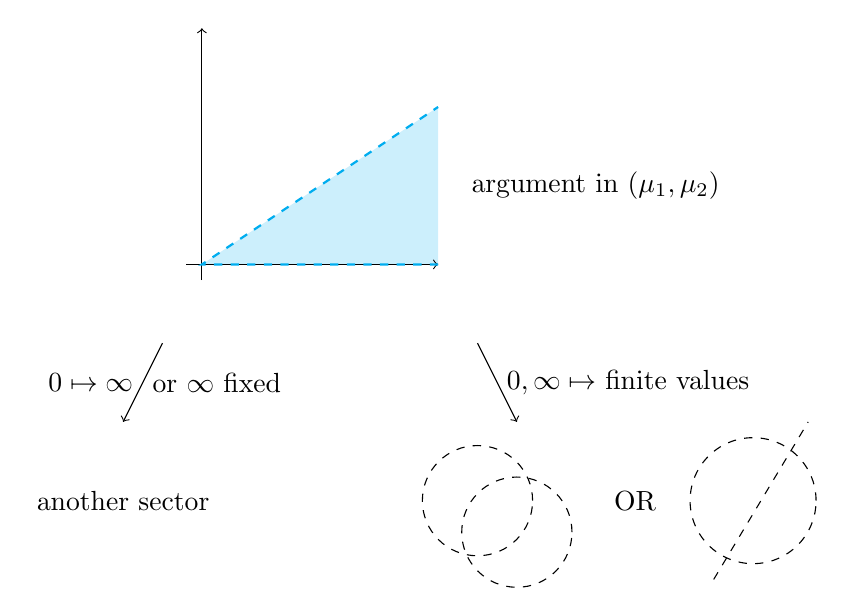
\begin{tikzpicture}
                    \fill[cyan!20] (3,0)--(0,0)--(3,2);
                    \draw[->] (-0.2,0)--(3,0);
                    \draw[->] (0,-0.2)--(0,3);
                    \draw[dashed,thick,cyan] (3,0)--(0,0)--(3,2);
                    \node at (5,1) {argument in \((\mu_1,\mu_2)\)};
                    \draw[->] (-0.5,-1)--node[left]{\(0\mapsto\infty\)}node[right]{or \(\infty\) fixed}(-1,-2);
                    \node at (-1,-3){another sector};
                    \draw[->] (3.5,-1)--node[right]{\(0,\infty\mapsto\) finite values}(4,-2);
                    \draw[dashed] (3.5,-3) circle (0.7);
                    \draw[dashed] (4,-3.4) circle (0.7);
                    \node at (5.5,-3) {OR};
                    \draw[dashed] (7,-3) circle (0.8);
                    \draw[dashed] (6.5,-4)--(7.7,-2); 
                \end{tikzpicture}
            \end{figure}

            In general, \(\{z\in\mathbb{C}\mid\arg(\frac{z-\alpha}{z-\beta})\in(\mu_1,\mu_2)\}\) gives a region bound by circles and lines.
        \end{enumerate}

        These are all examples of the Riemann mapping theorem.
        \begin{thm}[Riemann mapping theorem]
            Let \(U\subsetneq\CC\) be a simply connected domain, then \(U\) is conformally equivalent to \(D(0,1)\).        
        \end{thm}
    \end{exs}

    \begin{defn}
        A subset \(U\subseteq\CC\) is \textit{simply connected} if any simple closed (endpoints coincide) curve (loop) in \(U\) can be continuously contracted to a constant path (a point) in \(U\), i.e. \(U\) is path connected and for any \(\gamma:S^1\to U\), there exists an extended continuous map \(\hat{\gamma}:D^2\to U\) such that \(\hat{\gamma}|_{S_1}=\gamma\). Here, \(S^1\) and \(D^2\) denote the unit circle and closed unit disk respectively.
    \end{defn}
    \begin{figure}[ht!]
        \centering
        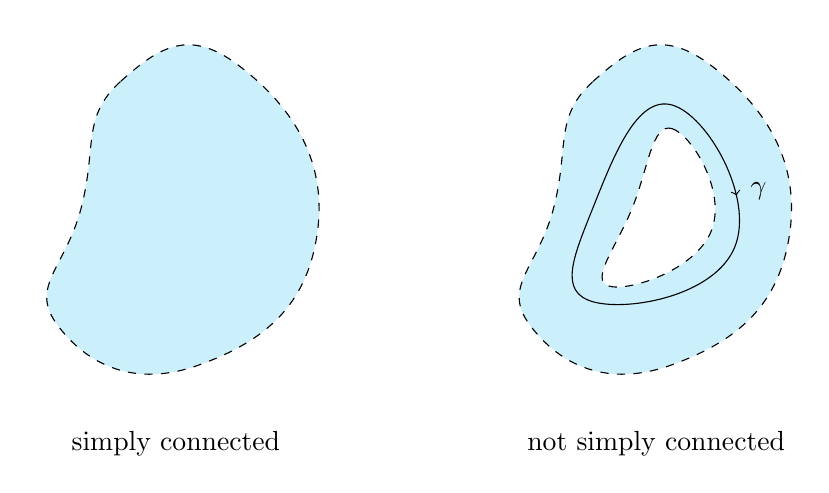
\begin{tikzpicture}
            \draw[fill=cyan!20,dashed] plot[smooth cycle,tension = 0.9] coordinates {(0,0) (0.5,1.6) (2,1.8) (3,-0.3) (1.5,-2) (-0.3,-1.5)};
            \draw[fill=cyan!20,dashed] plot[smooth cycle,tension = 0.9] coordinates {(6,0) (6.5,1.6) (8,1.8) (9,-0.3) (7.5,-2) (5.7,-1.5)};
            \draw[dashed,fill=white] plot[smooth cycle,tension = 0.9] coordinates {(7,0) (7.5,1) (8,-0.3) (6.7,-1)};
            \draw[decoration={markings, mark=at position 0.2 with {\arrow{>}}},postaction={decorate}] plot[smooth cycle,tension = 0.9] coordinates {(6.5,0) (7.5,1.3) (8.3,-0.5) (6.5,-1.2)};
            \node at (8.6,0.2) {\(\gamma\)};
            \node at (1.2,-3) {simply connected};
            \node at (7.3,-3) {not simply connected};
        \end{tikzpicture}
    \end{figure}
    \subsection{Power Series}
    \begin{rec}
        \begin{enumerate}[topsep=0pt,label=(\roman*)]
            \item A sequence \(\{f_n\}\) of functions converges uniformly to a function \(f\) on some set \(S\) if \(\forall\epsilon>0\), \(\exists M\in\NN\) such that \(\forall x\in S\), \(\abs{f_n(x)-f(x)}<\epsilon\) \(\forall n\ge N\).
            \item The uniform limit of continuous functions is continuous.
            \item Weierstrass M-test. If \((M_n)_{n\ge 0}\in \RR_{\ge 0}\) and \(0\le\abs{f_n(z)}\le M_n\) \(\forall z\in S\) and all \(n\in\NN\) sufficiently large, then
            \[\sum_{n=0}^{\infty}M_n<\infty\implies\sum_{n=1}^{\infty}f_n(z)\text{ converges uniformly on }S\,.\]
        \end{enumerate}
    \end{rec}
    Let \((c_n)_{n\in\NN\cup\{0\}}\subset\CC\) and fix \(a\in\CC\). Then for the series
    \[z\mapsto\sum_{n=0}^{\infty}c_n(z-a)^n\,,\]
    there is a unique \(R\in[0,\infty]\) such that the series converges absolutely, on \(\abs{z-a}<R\), and if \(0<r<R\), the series converges uniformly on \(\abs{z-a}\le r<R\). \(R\) is the radius of convergence of the series.
    \[R=\frac{1}{\lambda}\,,\text{ where }\lambda=\limsup_{n\to\infty}\abs{c_n}^{1/n}\,.\]
    \begin{thm}
        Let \(f(z)=\sum_{n=0}^{\infty} c_n(z-a)^n\) be a complex power series with radius of convergence \(R\). Then
        \begin{enumerate}[topsep=0pt,label=(\roman*)]
            \item \(f\) is holomorphic on \(D(a,R)\).
            \item \(f'(z)=\sum_{n=1}^{\infty}nc_n(z-a)^{n-1}\) with radius of convergence \(R\).
            \item \(f\) has derivatives of all orders. \(f^{(n)}(a)=n!c_n\).
        \end{enumerate}
    \end{thm}
    \begin{proof}
        Consider the function \(z\mapsto\sum_{n=1}^{\infty}nc_n(z-a)^{n-1}\). WLOG, can set \(a=0\). Since \(\abs{nc_n}\ge\abs{c_n}\), this series has radius of convergence \(R'\le R\). If \(0<R_1<R\), then for \(\abs{z}<R_1\), we have
        \[\abs{nc_nz^{n-1}}\le n\abs{c_n}R_1^{n-1}\frac{\abs{z}^{n-1}}{R_1^{n-1}}\,.\]
        Since \(n\cdot\frac{\abs{z}^{n-1}}{R_1^{n-1}}\to 0\) as \(n\to\infty\), for \(n\) suitably large, \(\abs{c_n}R_1^{n-1}\) provides an upper bound for \(\abs{nc_n z^{n-1}}\). By Weierstrass M-test (compare to \(f\)), we see  that \(\sum_{n=1}^{\infty}nc_n(z-a)^{n-1}\) converges absolutely and uniformly on \(0<\abs{z-a}<R_1\), so the radius of convergence of the series is \(R\).

        Consider
        \begin{align*}
            \frac{f(z)-f(w)}{z-w}&=\sum_{n=0}^{\infty}c_n\frac{z^n-w^n}{z-w}\\
            &=\lim_{N\to\infty}\sum_{n=0}^{N}c_n\left[\sum_{j=0}^{n-1}z_j w^{n-1-j}\right]\,.\tag{\(*\)}
        \end{align*}
        For \(\abs{z},\abs{w}<r<R\), we have
        \[\abs{c_n\left[\sum_{j=0}^{n-1}z_jw^{n-1-j}\right]}<\abs{c_n}\cdot n\cdot r^{n-1}\,,\]
        so (\(*\)) converges uniformly on \(\abs{z},\abs{w}<r\). So the series has a continuous limit. Call it \(g(z,w)\). When \(z=w\), \(g(z,z)=\sum_{n=0}^{\infty}nc_nz^{n-1}\). Therefore, \(f\) is differentiable with this derivative. This proves (i) and (ii), and (iii) is induction.\qed
    \end{proof}
    \begin{cor}
        If \(f(z)=\sum c_n(z-a)^n\) with radius of convergence \(R\) and \(\exists 0<\epsilon<R\) such that \(f(z)=0\) on \(D(a,\epsilon)\), then \(f(z)=0\) on \(D(a,R)\).
    \end{cor}
    \begin{proof}
        \(f=0\) on a neighbour of \(a\implies f^{(n)}(a)=0\) \(\forall n\in\NN\). We have \(c_n=0\) \(\forall n\), and so \(f=0\) on \(D(a,R)\).\qed 
    \end{proof}
    \subsection{The Exponential and Logarithm}
    \begin{defn}
        The exponential function is defined as
        \[ \ee^z\equiv \exp(z)\coloneqq \sum_{n=0}^{\infty}\frac{z^n}{n!}\,. \]
    \end{defn}
    \begin{rems}
        \begin{enumerate}[topsep=0pt,label=(\roman*)]
            \item The radius of convergence of \(\exp(z)\) is \(\infty\): \(\ee^z\) is entire and \(\dv{}{z}\ee^z=\ee^z\).
            \item For all \(z,w\in\CC\), \(\ee^{z+w}=\ee^z\cdot \ee^w\).
            \begin{proof}
                Fix \(w\in\CC\), and consider the function \(\ee^{z+w}\cdot \ee^{-z}\). This function has derivative \(\ee^{z+w}\ee^{-z}-\ee^{z+w}\ee^{-z}=0\), so constant. At \(z=0\), this function takes the value \(\ee^w\), so \(\ee^{z+w}=\ee^{z}\ee^{w}\) \(\forall z\in\CC\).\qed
            \end{proof}
            Notice that \(\ee^z\cdot \ee^{-z}=\ee^0=1\). Exponential never takes the value 0.
            \item \(z=x+\ii y\), \(x,y\in\RR\), then \(\ee^{z}=\ee^{x}\ee^{\ii y}\), \(\ee^{\ii y}=\cos y+\ii\sin y\), so
            \[\abs{\ee^{\ii y}}^2=\cos^2 y+\sin^2 y=1\,.\]
            \(\ee^z=\ee^x(\cos y+\ii\sin y)\) and \(\abs{\ee^z}=\ee^x=\ee^{\Re(z)}\). We see that \(\ee^{\ii \cdot 2\pi k}=1\) \(\forall k\in\ZZ\). More generally, \(\ee^{z+2\pi k\ii}=\ee^z\) \(\forall k\in\ZZ\).
            \begin{figure}[ht!]
                \centering
                \begin{tikzpicture}
                    \draw[->] (-2,0)--(2,0);
                    \draw[->] (0,-2)--(0,2);
                    \draw[red,dashed] (1,-2)node[below]{\(x=a\)}--(1,2);
                    \draw[cyan,dashed] (-1,-2)node[below]{\(x=b\)}--(-1,2);
                    \draw[fill=black] (1,0.2) circle (0.03) node[right]{\(z\)};
                    \draw[fill=black] (1,1.2) circle (0.03) node[right]{\(z+2\pi \ii\)};
                    \draw[fill=black] (1,-0.8) circle (0.03) node[right]{\(z-2\pi \ii\)};
                    \draw[fill=black] (1,-1.8) circle (0.03) node[right]{\(z-4\pi \ii\)};
                    \draw[->] (3,0) to [bend left=12] node[above]{\(z\mapsto \ee^z\)}(5,0);
                    \draw[->] (6,0)--(10,0);
                    \draw[->] (8,-2)--(8,2);
                    \draw[cyan,dashed] (8,0) circle (0.6);
                    \draw[cyan] (8.6,0.03)--(8.6,-0.03)node[below]{\(\ee^b\)};
                    \draw[red,dashed] (8,0) circle (1.6);
                    \draw[red] (9.6,0.03)--(9.6,-0.03)node[below right]{\(\ee^a\)};
                    \draw[fill=black] (8.494,1.522) circle (0.03)node[right]{\(w=\ee^z\)};
                \end{tikzpicture}
            \end{figure}
        \end{enumerate}
    \end{rems}
    \begin{defn}
        Let \(U\subset\CC^*\) be open. We say a function \(\lambda:U\to\CC\) which is continuous, is \textit{a branch of logarithm} if \(\forall z\in U\), \(\exp(\lambda(z))=z\).
    \end{defn}
    \begin{ex}
        \(U=\CC\setminus\RR_{\le 0}\). Define
        \[ \Log(z)=\ln\abs{z}+\ii\theta\,,\;\text{where }\theta=\Arg(z)\,,\;\theta\in(-\pi,\pi)\,.\]
        We call \(\Log\) \textit{the principal branch of the logarithm}. 
    \end{ex}
    \begin{figure}[ht!]
        \centering
        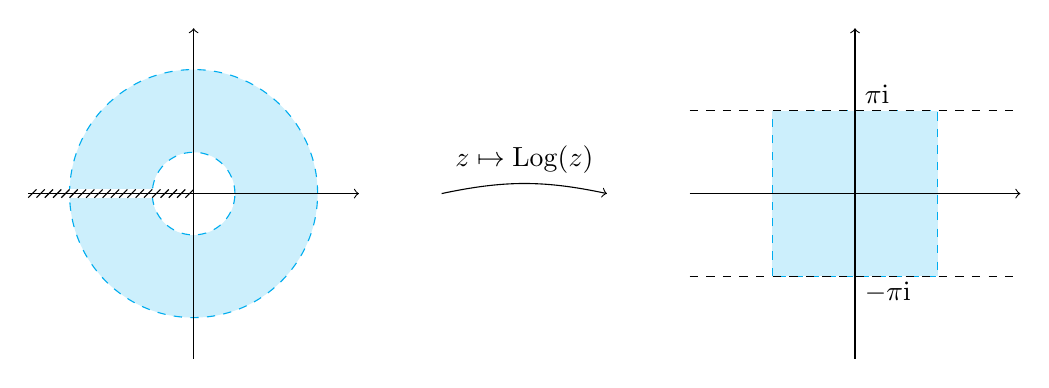
\begin{tikzpicture}[scale=1.05]
            \draw[cyan,fill=cyan!20,dashed] (0,0) circle (1.5);
            \draw[cyan,fill=white,dashed] (0,0) circle (0.5);
            \draw[white,fill=white] (-2,0.05)--(0,0.05)--(0,-0.05)--(-2,-0.05);
            \draw[->] (-2,0)--(2,0);
            \draw[->] (0,-2)--(0,2);
            \foreach \i in {1,...,20}{
                \draw (-0.1*\i,-0.05)--(0.1-0.1*\i,0.05);
            }
            \draw[->] (3,0) to [bend left=12] node[above]{\(z\mapsto \Log(z)\)}(5,0);
            \draw[cyan,fill=cyan!20,dashed] (7,-1) rectangle (9,1);
            \draw[->] (6,0)--(10,0);
            \draw[->] (8,-2)--(8,2);
            \draw[dashed] (6,1)--(10,1);
            \draw[dashed] (6,-1)--(10,-1);
            \node at (8,1.2)[right]{\(\pi \ii\)};
            \node at (8,-1.2)[right]{\(-\pi \ii\)};
        \end{tikzpicture}
    \end{figure}
    \begin{prop}
        \(\Log(z)\) is holomorphic on \(U\), with \(\dv{}{z}\Log(z)=\frac{1}{z}\). If \(\abs{z}<1\), then
        \[\Log(1+z)=\sum_{n=1}^{\infty}\frac{(-1)^{n-1}z^n}{n}\,.\]
    \end{prop}
    \begin{proof}
        A continuous inverse of \(\exp\) is holomorphic, so \(\Log\) is holomorphic on \(U\), and by computation of the inverse's derivative, \(\dv{}{z}\Log z=\frac{1}{z}\). We have that
        \[\dv{}{z}\Log(1+z)=\frac{1}{z+1}=1-z+z^2-z^3+\dots\]
        This power series is the derivative of \(\sum_{n=1}^{\infty}\frac{(-1)^{n+1}z^n}{n}\), so
        \[\Log(1+z)=\sum_{n=1}^{\infty}\frac{(-1)^{n+1}z^n}{n}+\text{const.}\]
        Evaluating at \(z=0\), we have \(\text{const.}=0\).\qed
    \end{proof}
    \begin{defn}
        For \(z,\alpha\in\CC\), the multivalued function
        \[z^\alpha\coloneqq\exp(\alpha\log z)\,,\;\text{where }\log z=\ln\abs{z}+\ii\arg(z)\,.\]
        The single-valued function is
        \[z^\alpha\coloneqq\exp(\alpha\Log z)\,,\;\text{where }z\in\CC\setminus\RR_{\le 0}\,.\]
    \end{defn}
    Note that the multivalued function is single-valued if \(\alpha\in\ZZ\), and is finitely multivalued if \(\alpha\in\QQ\). Let \(\alpha=\frac{a}{b}\in\mathbb{Q}\), then the values of \(z^\alpha\) differ by a \(b^{th}\) root of unity.
    \begin{ex}
        \(\alpha=\frac{1}{2}\). \(z^{1/2}\) takes two opposite values for a given non-zero \(z\), which are negative of each other.
    \end{ex}
    \begin{cau}
        It need not hold for single-valued \(z^\alpha\) such that \((zw)^\alpha=z^\alpha w^\alpha\). E.g. \(\alpha=\frac{1}{2}\).
        \begin{figure}[ht!]
            \centering
            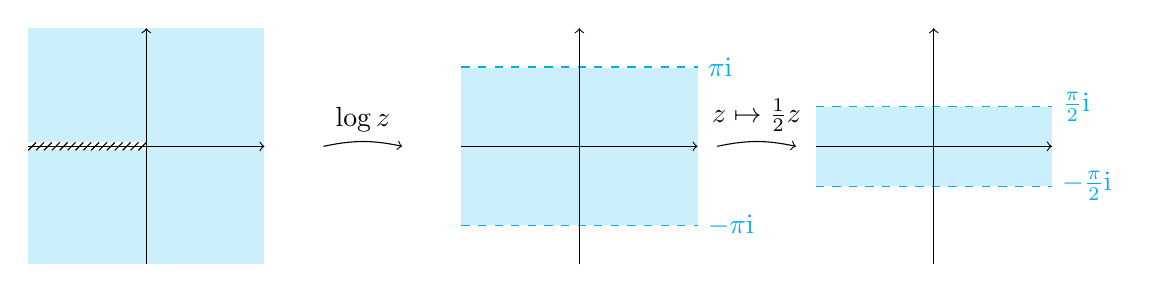
\begin{tikzpicture}
                \fill[cyan!20] (-1.5,-1.5) rectangle (1.5,1.5);
                \fill[white] (-1.5,-0.05) rectangle (0,0.05);
                \draw[->] (-1.5,0)--(1.5,0);
                \draw[->] (0,-1.5)--(0,1.5);
                \foreach \i in {1,...,15}{
                    \draw (-0.1*\i,-0.05)--(0.1-0.1*\i,0.05);
                }
                \draw[->] (2.25,0) to [bend left=12] node[above]{\(\log z\)}(3.25,0);
                \draw[cyan,dashed,thick] (4,1)--(7,1)node[right]{\(\pi \ii\)};
                \draw[cyan,dashed,thick] (4,-1)--(7,-1)node[right]{\(-\pi \ii\)};
                \fill[cyan!20] (4,-1) rectangle (7,1);
                \draw[->] (4,0)--(7,0);
                \draw[->] (5.5,-1.5)--(5.5,1.5);
                \draw[->] (7.25,0) to [bend left=12] node[above]{\(z\mapsto \frac{1}{2}z\)}(8.25,0);
                \draw[cyan,dashed,thick] (8.5,0.5)--(11.5,0.5)node[right]{\(\frac{\pi}{2}\ii\)};
                \draw[cyan,dashed,thick] (8.5,-0.5)--(11.5,-0.5)node[right]{\(-\frac{\pi}{2}\ii\)};
                \fill[cyan!20] (8.5,-0.5) rectangle (11.5,0.5);
                \draw[->] (8.5,0)--(11.5,0);
                \draw[->] (10,-1.5)--(10,1.5);
            \end{tikzpicture}
        \end{figure}

        \(-\frac{\pi}{2}<\Im z<\frac{\pi}{2}\) maps under \(\exp\) to the right half plane
        \begin{figure}[ht!]
            \centering
            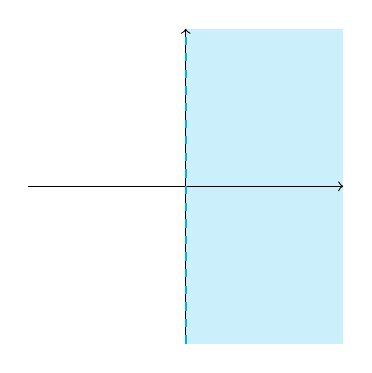
\begin{tikzpicture}
                \fill[cyan!20] (0,-2)rectangle(2,2);
                \draw[->] (-2,0)--(2,0);
                \draw[->] (0,-2)--(0,2);
                \draw[dashed,thick,cyan] (0,-2)--(0,2);
            \end{tikzpicture}
        \end{figure}\\
        but two numbers in right half plane need not have their product in the right half plane.
    \end{cau}

    Following \(\log z\) around a loop about \(0\): \(\log z=\ln\abs{z}+\ii\arg z\). \(\arg z\) increases by \(2\pi\) as we travel the loop, so there is no continuous branch of log on any loop about 0, or any neighbourhood of 0.

    \begin{ex}
        Consider \(f(z)=\sqrt{z(z-1)}\) defined on \(\CC\setminus[0,1]\).
        
        As we travel around the loop, \(\arg(z(z-1))\) increases by \(4\pi\) as we travel around the loop, so \(\exp(\frac{1}{2}\log(z(z-1)))\) is independent of the choice of argument for \(z(z-1)\).
        \begin{figure}[ht!]
            \centering
            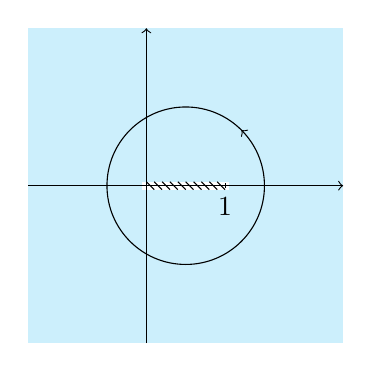
\begin{tikzpicture}
                \fill[cyan!20] (-1.5,-2)rectangle(2.5,2);
                \fill[white] (-0.05,-0.05) rectangle (1.05,0.05);
                \draw[->] (-1.5,0)--(2.5,0);
                \draw[->] (0,-2)--(0,2);
                \draw (1,0.03)--(1,-0.03)node[below]{1};
                \foreach \i in {1,...,10}{
                    \draw (0.1*\i,-0.05)--(0.1*\i-0.1,0.05);
                }
                \draw[decoration={markings, mark=at position 0.125 with {\arrow{>}}},postaction={decorate}] (0.5,0) circle (1);
            \end{tikzpicture}
        \end{figure}
    \end{ex}

    \newpage
    \section{Contour Integration}
    \begin{defn}
        If \(f:[a,b]\to\CC\) is continuous (so \(\Re f\), \(\Im f\) are integrable), we define
        \[\int_{a}^{b}f(t)\dd{t}=\int_{a}^{b}\Re f(t)\dd{t}+\ii\int_{a}^{b}\Im f(t)\dd{t}\,.\]
    \end{defn}
    \begin{prop}
        If \(f:[a,b]\to\CC\) is continuous, then
        \[\abs{\int_{a}^{b}f(t)\dd{t}}\le(b-a)\sup_{a\le t\le b}\abs{f(t)}\,.\]
    \end{prop}
    \begin{proof}
        Let \(\theta=\arg(\int_{a}^{b}f(t)\dd{t})\).
        \begin{align*}
            \abs{\int_{a}^{b}f(t)\dd{t}}&=\ee^{-\ii \theta}\int_{a}^{b}f(t)\dd{t}\\
            &=\int_{a}^{b}\parunderbrace{\ee^{-\ii \theta}f(t)}{\text{complex function with real integral}}\dd{t}\\
            &=\int_{a}^{b}\Re[\ee^{-\ii \theta} f(t)]\dd{t}\qquad(\text{by definition})\\
            &\le \int_{a}^{b}\abs{\ee^{-\ii \theta}f(t)}\dd{t}=\int_{a}^{b}\abs{f(t)}\dd{t}\tag{\(\dagger_1\)}\\
            &\le\sup_{t\in[a,b]}\abs{f(t)}\cdot(b-a)\,.\tag{\(\dagger_2\)}
        \end{align*}\qed
    \end{proof}
    Note we have \(\abs{\int_a^b f(t)\dd{t}}=\sup_{t\in[a,b]}\abs{f(t)}\cdot(b-a)\)
    \[\iff\text{ both }(\dagger_1)\text{ and }(\dagger_2)\text{ are equality.}\]
    By continuity of \(f\), \((\dagger_2)\) an equality \(\iff\abs{f(t)}\equiv\sup_{t\in[a,b]}\abs{f(t)}\), and \((\dagger_1)\) an equality \(\iff\arg f(t)\equiv\theta\), so \(f\) is a constant.

    \begin{defn}
        Let \(\gamma\) be a \(C^1\)-smooth curve \(\gamma:[a,b]\to\mathbb{C}\). Then define the arc length of \(\gamma\) to be
        \[\length(\gamma)\coloneqq\int_{a}^{b}\abs{\gamma'(t)}\dd{t}\,.\]
        If \(f:U\to\CC\) is continuous, and \(\gamma:[a,b]\to U\) is \(C^1\) smooth, then the integral of \(f\) along \(\gamma\) is
        \[\int_\gamma f(z)\dd{z}\coloneqq\int_{a}^{b}f(\gamma(t))\gamma'(t)\dd{t}\,.\]
    \end{defn}
    \begin{ppts}
        \begin{enumerate}[topsep=0pt,label=(\roman*)]
            \item Linearity. \(\int_\gamma c_1f_1+c_2f_2=c_1\int_\gamma f_1+c_2\int_\gamma f_2\).
            \item If \(a<a'<b\), then
            \[\int_{\gamma|_{[a,b]}}f=\int_{\gamma|_{[a,a']}}f+\int_{\gamma|_{[a',b]}}f\,.\]
            \item If \((-\gamma)(t)=\gamma(-t):[-b,-a]\to U\), then
            \[\int_{-\gamma}f(z)\dd{z}=-\int_\gamma f(z)\dd{z}\,.\]
            \item Independence of parameterisation: if \(\phi:[a',b']\to[a,b]\) is \(C^1\)-smooth, \(\phi(a')=a\) and \(\phi(b')=b\), then \(\delta=\gamma\circ\phi:[a',b']\to U\) satisfies
            \[\int_{\delta}f(z)\dd{z}=\int_\gamma f(z)\dd{z}\,.\]
            So we will often assume \([a,b]=[0,1]\).
        \end{enumerate}
    \end{ppts}

    We can allow piecewise-\(C^1\)-smooth paths, i.e. \(a=a_0<a_1<\dots<a_n=b\) such that \(\gamma_i=\gamma|_{[a_{i-1},a_i]}\) is \(C^1\)-smooth, and \(\gamma\) is continuous. Then we define
    \[\int_{\gamma}f=\sum_{i=1}^{n}\int_{\gamma_i}f\,.\]
    This is well-defined by the additivity of paths and independence of parameterisation.

    \begin{rem}
        Any piecewise-\(C^1\)-smooth curve can be reparameterised to be \(C^1\)-smooth. For such a \(\gamma\), replace \(\gamma_1\) by \(\gamma_i\circ h_i\) where \(h_i\) is a monotonic \(C^1\)-smooth bijection with endpoint derivatives 0. An example is
        \[\gamma(t)=\begin{cases}
            1+\ii\sin(\pi t) &t\in[0,\frac{1}{2}]\\
            \sin(\pi t)+\ii & t\in[\frac{1}{2},1] 
        \end{cases}\]
        is \(C^1\)-smooth.
        \begin{figure}[ht!]
            \centering
            \begin{tikzpicture}[decoration={markings,mark=at position 0.5 with {\arrow{>}}}]
                \draw[->] (-0.2,0)--(2,0);
                \draw[->] (0,-0.2)--(0,2);
                \draw[postaction={decorate}] (1.4,0)--(1.4,1.4);
                \draw[postaction={decorate}] (1.4,1.4)--(0,1.4);
                \draw[fill=black] (1.4,1.4) circle (0.04) node[right]{\(1+\ii\)};
            \end{tikzpicture}
        \end{figure}
    \end{rem}
    \begin{term}
        A \textit{curve} is a piecewise-\(C^1\)-smooth path, and a \textit{contour} is a simple (injective except at end points), closed (\(\gamma(a)=\gamma(b)\)), piecewise-\(C^1\)-smooth path.
    \end{term}
    \begin{prop}
        For any continuous \(f:U\to\CC\), \(U\) open, and for any curve \(\gamma:[a,b]\to U\),
        \[\int_\gamma f\le\length(\gamma)\cdot\sup_{z\in\gamma}\abs{f(z)}\,.\]
    \end{prop}
    \begin{proof}
        \begin{align*}
            \abs{\int_\gamma f}&=\abs{\int_{a}^{b}f(\gamma(t))\gamma'(t)\dd{t}}\\
            &=\int_{a}^{b}\abs{f(\gamma(t))}\abs{\gamma'(t)}\dd{t}\qquad(\text{rotational trick})\\
            &\le\sup_{t\in[a,b]}\abs{f(\gamma(t))}\int_{a}^{b}\abs{\gamma'(t)}\dd{t}\\
            &=\sup_{z\in\gamma}\abs{f(z)}\cdot\length(\gamma)\,.
        \end{align*}\qed
    \end{proof}
    \begin{cor}
        If \(f_n:U\to\CC\) continuous on open \(U\) for \(n\in\NN\), and \(f:U\to\CC\) continuous with \(f_n\to f\) uniformly on a curve \(\gamma\) in \(U\), then
        \[\int_\gamma f_n(z)\dd{z}\to\int_{\gamma}f(z)\dd{z}\text{ as }n\to\infty\,.\]
    \end{cor}
    \begin{proof}
        \begin{align*}
            \abs{\int_\gamma f_n-\int_\gamma f}&=\abs{\int_\gamma f_n-f}\\
            &=\length(\gamma)\cdot\sup_{z\in\gamma}\abs{f_n(z)-f(z)}\\
            &\to 0\text{ as }n\to\infty\text{ by uniform convergence.}
        \end{align*}\qed
    \end{proof}
    \begin{keyex}
        \(f(z)=z^n\) where \(n\in\ZZ\). Let \(U=\CC^*\) and \(\gamma(t):[0,2\pi]\to U\) be \(\gamma(t)=\ee^{\ii t}\). Then
        \begin{align*}
            \int_\gamma f(z)\dd{z}&=\int_{0}^{2\pi}\ee^{n\ii t}\ii\ee^{\ii t}\dd{t}\\
            &=\ii\int_{0}^{2\pi}\ee^{(n+1)\ii t}\dd{t}\\
            &=\ii\int_{0}^{2\pi}\cos((n+1)t)+\ii\sin((n+1)t)\dd{t}\,.
        \end{align*}
        This integral vanishes unless \(n=-1\), in which case we have \(\ii\int_{0}^{2\pi}\dd{t}=2\pi \ii\). So
        \begin{align*}
            \int_{\text{unit circle}}z^n\dd{z}=\begin{cases}
                2\pi \ii& \text{if }n=-1\\
                0 & \text{if }n\ne -1\,.
            \end{cases}
        \end{align*}
    \end{keyex}
    \subsection{Fundamental Theorem of Calculus}
    \begin{thm}[Fundamental theorem of calculus]
        If \(f:U\to\CC\) is continuous on an open \(U\subset\CC\), and \(f=F'\) on \(U\); that is, \(F\) is an antiderivative for \(f\) on \(U\). Then for any curve \(\gamma:[a,b]\to U\),
        \[\int_\gamma f(z)\dd{z}=F(\gamma(b))-F(\gamma(a))\,,\]
        and so \(\int_{\gamma}f(z)\dd{z}=0\) if \(\gamma\) is closed.
    \end{thm}
    \begin{proof}
        We have
        \begin{align*}
            \int_\gamma f(z)\dd{z}&=\int_{a}^{b}f(\gamma(t))\gamma'(t)\dd{t}\\
            &=\int_{a}^{b}F(\gamma(t))'\dd{t}\\
            &=F(\gamma(b))-F(\gamma(a))
        \end{align*}
        by the real fundamental theorem of calculus.\qed
    \end{proof}
    Putting these together, with computation of \(\int_{\text{unit circle}}\frac{1}{z}\dd{z}\ne 0\), we see that \(\frac{1}{z}\) has no holomorphic antiderivative on any neighbourhood of any circle centred at 0.
    \begin{thm}[Converse of FTC]
        If \(f:U\to\CC\) is continuous on a domain \(U\), and \(\int_\gamma f=0\) \(\forall\) closed curve \(\gamma\in U\), then \(\exists\) holomorphic \(F:U\to\CC\) with \(F'=f\).
    \end{thm}
    \begin{proof}
        Choose \(a_0\in U\). For each \(w\in U\), choose a path \(\gamma_w\) from \(a_0\) to \(w\), and define
        \[ F(w)=\int_{\gamma_w}f(z)\dd{z}\,.\]
        Notice that if \(\gamma_w'\) were another such path, then
        \[\int_{\gamma_w}f-\int_{\gamma_w'}f=\int_{\gamma_w-\gamma_w'}f=0\]
        by hypothesis. So \(F\) is independent of the path choice so it is well defined. Given \(w\in U\), find \(r_w>0\) such that \(D(w,r_w)\subseteq U\). For \(\abs{h}<r_w\), define \(\delta_h:[0,1]\to U\) to be the line segment from \(w\) to \(w+h\).
        \begin{center}
            \centering
            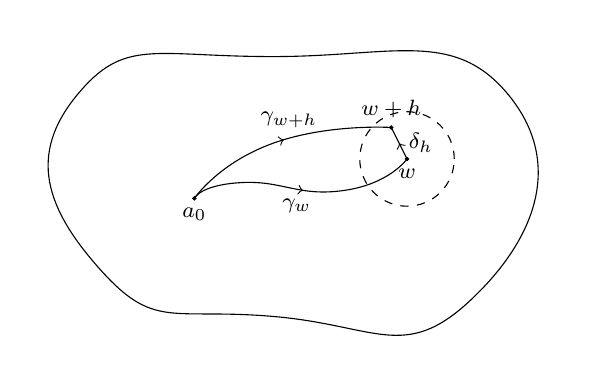
\begin{tikzpicture}[decoration={markings,mark=at position 0.5 with {\arrow{>}}}] 
                \draw plot[smooth cycle, tension=1] coordinates {(0,1.5) (3,1) (2.5,-1.6) (0,-1.8) (-2.2,-1.2) (-2.5,1)};
                \draw[fill=black] (-1,-0.3) circle (0.02) node[below]{\footnotesize \(a_0\)};
                \draw[fill=black] (1.7,0.2) circle (0.02) node[below]{\footnotesize \(w\)};
                \draw[fill=black] (1.5,0.6) circle (0.02) node[above]{\footnotesize \(w+h\)};
                \draw[dashed] (1.7,0.2) circle (0.6);
                \draw[postaction={decorate}] plot[smooth, tension=1] coordinates {(-1,-0.3) (-0.4,-0.1) (0.9,-0.2) (1.7,0.2)};
                \draw[postaction={decorate}] plot[smooth, tension=1] coordinates {(-1,-0.3) (0,0.4) (1.5,0.6)};
                \draw[postaction={decorate}] (1.7,0.2)--(1.5,0.6);
                \node at (1.6,0.4)[right]{\footnotesize \(\delta_h\)};
                \node at (0.3,-0.4){\footnotesize \(\gamma_w\)};
                \node at (0.2,0.7){\footnotesize \(\gamma_{w+h}\)};
            \end{tikzpicture}
        \end{center}

        We have
        \[F(w+h)=\int_{\gamma_{w+h}}f=\int_{\gamma_w}f+\int_{\delta_h}f\]
        by hypothesis, so
        \begin{align*}
            F(w+h)&=F(w)+\int_{\delta_h}f(z)\dd{z}\\
            &=F(w)+hf(w)+\int_{\delta_h}f(z)-f(w)\dd{z}\,.
        \end{align*}
        Noting \(\int_{\delta_h}f(w)\dd{z}=hf(w)\), so
        \begin{align*}
            \abs{\frac{F(w+h)-F(w)}{h}-f(w)}&=\abs{\frac{1}{h}\int_{\delta h}f(z)-f(w)\dd{z}}\\
            &=\frac{\length(\delta h)}{\abs{h}}\sup_{z\in\delta h}\abs{f(z)-f(w)}\\
            &=\sup_{z\in D(w,r_w)}\abs{f(z)-f(w)}\to 0\text{ as }r_w\to 0\,.
        \end{align*}
        Therefore, \(F'(w)=f(w)\).\qed
    \end{proof}
    \subsection{Cauchy's Theorem}
    \begin{defn}
        An open subset \(U\subset\CC\) is \textit{convex} if \(\forall a,b\in U\), the segment from \(a\) to \(b\) is in \(U\). We say \(U\) is \textit{starlike} if \(\exists a_0\in U\) such that \(\forall a\in U\), the segment from \(a_0\to a\) is in \(U\).
    \end{defn}
    \[\{\text{disks}\}\subsetneq\{\text{convex domains}\}\subsetneq\{\text{starlike domains}\}\subsetneq\{\text{simply connected domains}\}\subsetneq\{\text{domains}\}\,.\]
    \begin{lem}
        Suppose \(U\) is a starlike domain, and \(f:U\to\CC\) is continuous, and for all triangles \(T\) in \(U\), \(\int_{\partial T}f=0\), then \(f\) has an antiderivative in \(U\).
    \end{lem}
    \begin{proof}
        Same as previous, using segments from the base \(a_0\in U\) to define the antiderivative.\qed
    \end{proof}
    \begin{thm}
        \(f:U\to\CC\) holomorphic on an open \(U\subseteq\CC\), and \(T\) is a triangle in \(U\), then \(\int_{\partial T}f=0\).
    \end{thm}
    \begin{proof}
        Call \(I=\abs{\int_{\partial T}f}\) and \(L=\length(\partial T)\). Subdivide \(T\) by bisecting sides to obtain \(T_1,T_2,T_3,T_4\).

        \begin{figure}[ht!]
            \centering
            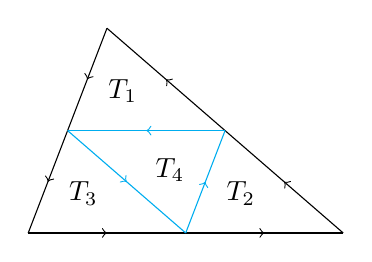
\begin{tikzpicture}[decoration={markings,mark=at position 0.5 with {\arrow{>}}}]
                \draw[postaction={decorate}] (0,0)--(2,0);
                \draw[postaction={decorate}] (2,0)--(4,0);
                \draw[postaction={decorate}] (4,0)--(2.5,1.3);
                \draw[postaction={decorate}] (2.5,1.3)--(1.0,2.6);
                \draw[postaction={decorate}] (1.0,2.6)--(0.5,1.3);
                \draw[postaction={decorate}] (0.5,1.3)--(0,0);
                \draw[cyan,postaction={decorate}] (0.5,1.3)--(2,0);
                \draw[cyan,postaction={decorate}] (2.5,1.3)--(0.5,1.3);
                \draw[cyan,postaction={decorate}] (2,0)--(2.5,1.3);
                \node at (0.7,0.5) {\(T_3\)};
                \node at (2.7,0.5) {\(T_2\)};
                \node at (1.8,0.8) {\(T_4\)};
                \node at (1.2,1.8) {\(T_1\)};
            \end{tikzpicture}
        \end{figure}

        We have \(\partial T-\partial T_4=\partial T_1+\partial T_2+\partial T_3\), so
        \[\int_{\partial T}f=\sum_{i=1}^{4}\int_{\partial T_i}f\,.\]
        By the triangle inequality, \(\exists i\in\{1,2,3,4\}\) such that
        \[\abs{\int_{\partial T_i}f}\ge \frac{1}{4}I\,.\]
        Call it \(T^{(1)}\) and note that its length is \(\length(T^{(1)})=\frac{L}{2}\). Proceeding in this way, we obtain a sequence of triangles
        \[ T\supseteq T^{(1)}\supseteq T^{(2)}\supseteq\dots\]
        with \(\length(T^{(n)})=\frac{L}{2^n}\) and
        \[\abs{\int_{\partial T^{(n)}}f}\ge \frac{1}{4^n}I\,.\]
        We have
        \[\bigcap_{n=1}^{\infty}T^{(n)}=\{w\}\]
        for some \(w\in T\subset U\). Note that functions \(g(z)=z\), \(h(z)=\text{const.}\) have holomorphic antiderivative everywhere, so they integrate to \(0\) on any closed curve by FTC. So for \(w\in U\),
        \[\int_{\partial T^{(n)}}f(z)\dd{z}=\int_{\partial T^{(n)}}f(z)-f(w)-(z-w)f'(w)\dd{z}\,.\]
        \(f\) is differentiable at \(w\), i.e. \(\forall\epsilon>0\), \(\exists\delta>0\) such that \(\abs{z-w}<\delta\),
        \[\abs{f(z)-f(w)-(z-w)f'(w)}<\epsilon\abs{z-w}\,.\]
        So given \(\epsilon>0\), \(\exists N\in\NN\) such that \(\forall n\ge N\), \(T^{(n)}\subseteq D(w,\delta)\), so
        \begin{align*}
            \abs{\int_{\partial T^{(n)}}f(z)\dd{z}}&=\abs{\int_{\partial T^{(n)}}f(z)-f(w)-(z-w)f'(w)\dd{z}}\\
            &\le\length(T^{(n)})\sup_{z\in\partial T^{(n)}}\epsilon\abs{z-w}\\
            &=\frac{L}{2^n}\epsilon\sup_{z\in\partial T^{(n)}}\abs{z-w}\le \frac{L^2}{2^{2n}}\epsilon\,.
        \end{align*}
        Therefore, \(I\le L^2\epsilon\to 0\) as \(\epsilon\to 0\), so \(I\to 0\).\qed
    \end{proof}
    \begin{thm}
        Let \(S\subset U\) be a finite subset of a domain \(U\), and \(f:U\to\CC\) continuous on \(U\) and holomorphic on \(U\setminus S\). Then for any triangle \(T\subset U\), \(\int_{\partial T}f=0\).
    \end{thm}
    \begin{proof}
        Using triangle subdivision, it suffices to assume at \(S=\{a\}\), \(a\in T\). If \(T\) has \(a\in T'\subset T\) for another triangle \(T'\), we can subdivide \(T\) into triangles, one of which is \(T'\).
        \begin{figure}[ht!]
            \centering
            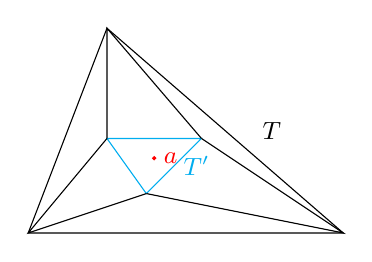
\begin{tikzpicture}
                \draw (0,0)--(4,0)--node[right=1em]{\small \(T\)}(1,2.6)--(0,0);
                \draw[cyan] (1.5,0.5)--node[right]{\small \(T'\)}(2.2,1.2)--(1,1.2)--(1.5,0.5);
                \draw (1,1.2)--(0,0)--(1.5,0.5);
                \draw (1.5,0.5)--(4,0)--(2.2,1.2);
                \draw (1,1.2)--(1,2.6)--(2.2,1.2);
                \draw[red,fill=red] (1.6,0.95) circle (0.02) node[right]{\small \(a\)};
            \end{tikzpicture}
        \end{figure}

        Since \(f\) is holomorphic on a neighbourhood of these triangles, except possibly \(T'\), the previous theorem implies that the integral vanish on their boundaries, so
        \[\int_{\partial T}f=\int_{\partial T'}f\,.\]
        Using basic estimation
        \[\abs{\int_{\partial T}f}=\abs{\int_{\partial T'}f}\le\length(\partial T')\cdot\sup_{z\in\partial T'}\abs{f(z)}\,,\]
        where the \(\sup\) is finite because \(f\) is continuous on \(U\). Let \(\length(\partial T')\to 0\), we have \(\int_{\partial T}f\to 0\).\qed
    \end{proof}
    \begin{thm}[Cauchy's theorem on a disk/starlike domain]
        Let \(D\) be a disk or any starlike domain, and \(f:D\to\CC\) continuous, holomorphic except at finitely many points. Then \(\int_{\gamma}f=0\) for any closed curve in \(D\).
        \begin{proof}
            By previous theorem, \(\int_{\partial T}f=0\) for all triangles \(T\) in \(D\), so by the converse of FTC for starlike domains, \(\exists\) antiderivatives \(F'=f\) in \(D\). By FTC, \(\int_\gamma f=0\) for all closed curves \(\gamma\).\qed
        \end{proof}
    \end{thm}
    \begin{thm}[Cauchy's integral formula]
        Let \(U\subseteq\CC\) be a domain, \(f:U\to\mathbb{C}\) holomorphic and \(\overline{D(a,r)}\subseteq U\). Then \(\forall z\in D(a,r)\),
        \[f(z)=\frac{1}{2\pi \ii}\int_{\partial D(a,r)}\frac{f(w)}{w-z}\dd{w}\,.\]
    \end{thm}
    \begin{proof}
        Define
        \[g(w)=\begin{cases}
            \frac{f(w)-f(z)}{w-z}-f'(z) & \text{for }w\ne z\\
            0 & \text{for }w=z\,.
        \end{cases}\]
        Then \(g\) is continuous at \(z\), holomorphic on \(D(a,r)\) except possibly at \(z\). Find \(r_1>0\) such that \(\overline{D(a,r)}\subseteq  D(a,r_1)\subseteq U\). Apply Cauchy's theorem to \(g\) and \(\gamma=\partial D(a,r)\), we have \(\int_{\partial D(a,r)}g(w)\dd{w}=0\), so
        \[\int_{\partial D(a,r)}\frac{f(w)}{w-z}\dd{w}=\int_{\partial D(a,r)}\frac{f(z)}{w-z}\dd{w}=f(z)\int_{\partial D(a,r)}\frac{\dd{w}}{w-z}\,.\]
        We need to show that the last integral is \(2\pi \ii\). On the contour, we have \(\abs{w-a}=r>\abs{z-a}\), so
        \[\frac{1}{w-z}=\frac{1}{(w-a)(1-\frac{z-a}{w-a})}=\sum_{n=0}^{\infty}\frac{(z-a)^n}{(w-a)^{n+1}}\]
        by geometric expansion. So
        \[\int_{\partial D(a,r)}\frac{1}{w-z}\dd{w}=\sum_{n=0}^{\infty}\left[(z-a)^n\int_{\partial D(a,r)}\frac{1}{(w-a)^{n+1}}\dd{w}\right]\,.\]
        We have shown that only the \(n=0\) term in non-vanishing, in which case the result is \(2\pi \ii\). Therefore, we have \(\int_{\partial D(a,r)}\frac{\dd{w}}{w-z}=2\pi \ii\), so
        \[f(z)=\frac{1}{2\pi \ii}\int_{\partial D(a,r)}\frac{f(w)}{w-z}\dd{w}\]
        as claimed.\qed
    \end{proof}
    \begin{figure}[ht!]
        \centering
        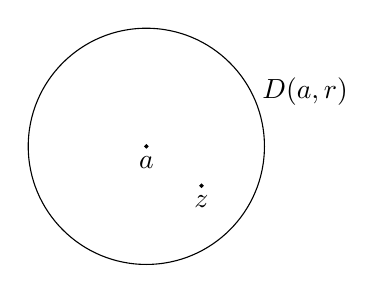
\begin{tikzpicture}
            \draw[fill=black] (0,0) circle (0.02)node[below]{\(a\)};
            \draw[fill=black] (0.7,-0.5) circle (0.02)node[below]{\(z\)};
            \draw (0,0) circle (1.5);
            \node at (1.35,0.7)[right]{\(D(a,r)\)};
        \end{tikzpicture}
    \end{figure}
    The value of \(f\) on \(\partial D(a,r)\implies\) value of \(f\) in \(D(a,r)\).
    \subsection{Applications of CIF}
    \begin{cor}[Mean-value property]
        If \(f:U\to\CC\) is holomorphic on a domain \(U\), and a disk \(D(a,r)\subseteq U\), then
        \[f(a)=\int_{0}^{1}f(a+re^{2\pi \ii t})\dd{t}\,,\]
        i.e. \(f\) takes the average value on the disk boundary at the centre.
    \end{cor}
    \begin{proof}
        Use CIF with \(t\mapsto re^{2\pi \ii t}\).\qed
    \end{proof}
    \begin{cor}[Local maximum principle]
        Let \(f:D(a,r)\to\CC\) be holomorphic. If \(\abs{f(z)}\le\abs{f(a)}\) \(\forall z\in D(a,r)\), then \(f\) is constant.        
    \end{cor}
    \begin{proof}
        By mean-value property, \(\forall 0<\rho<r\) we have
        \begin{align*}
            \abs{f(a)}&=\abs{\int_{0}^{1}f(a+\rho \ee^{2\pi \ii t})\dd{t}}\\
            &\le\sup_{\abs{z-a}=\rho}\abs{f(z)}\le \abs{f(a)}
        \end{align*}
        by hypothesis. So the inequalities are equalities if the hypothesis hold, and \(f\) is constant on \(\abs{z-a}=\rho\). So \(f\) is constant on \(D(a,r)^\times\implies f\) is constant.\qed
    \end{proof}
    \begin{thm}[Liouville's theorem]
        Every bounded entire function is constant.
    \end{thm}
    \begin{proof}
        Consider the value
        \[\abs{f(z)-f(0)}=\frac{1}{2\pi}\abs{\int_{\partial D(0,R)}f(w)\left[\frac{1}{w-z}-\frac{1}{w}\right]\dd{w}}\]
        for any \(R>\abs{z}\) by CIF. Let's choose \(R>2\abs{z}\), then
        \[\abs{\frac{1}{w-z}}<\frac{2}{R}\text{ and }\abs{\frac{1}{w}}=\frac{1}{R}\]
        for all \(w\in\partial D(0,R)\), so
        \begin{align*}
            \abs{f(z)-f(0)}&=\frac{1}{2\pi}\abs{\int_{\partial D(0,R)}f(w)\cdot\frac{z}{(w-z)w}\dd{w}}\\
            &\le\frac{1}{2\pi}\cdot2\pi R\cdot\sup_{w\in\partial D(0,R)}\abs{f(w)}\cdot\abs{z}\cdot\frac{2}{R}\cdot\frac{1}{R}\\
            &\le\sup_{w\in\CC}\abs{f(w)}\cdot\frac{2}{R}\cdot\abs{z}\to 0
        \end{align*}
        as \(R\to\infty\). So \(f(z)=f(0)\). Since \(z\) is arbitrary, \(f\) is constant.\qed
    \end{proof}
    \begin{cor}[The fundamental theorem of algebra]
        Every non-constant polynomial \(p(z)\in\CC[z]\) has a root in \(\CC\).
    \end{cor}
    \begin{proof}
        Suppose \(p\ne 0\) \(\forall z\in\CC\), then \(f(z)=\frac{1}{p(z)}\) is entire. \(p\) is non-constant \(\implies p(z)=a_dz^d+\dots +a_1z^1+a_0\), \(d\ge 1\), \(a_d\ne 0\), so \(\abs{p(z)}\to\infty\) as \(\abs{z}\to \infty\). So \(\abs{f(z)}\to 0\) as \(\abs{z}\to\infty\), and so \(\abs{f}\) is bounded since \(\abs{f}\) is bounded on any closed disk. Then by Liouville's theorem, \(f(z)\) is constant, so \(p\) is constant. Contradiction.\qed
    \end{proof}
    \begin{thm}[Higher order CIF]
        \(f:D(a,r)\to\CC\) holomorphic, then \(f\) is represented by a convergent power series on \(D(a,r)\)
        \[f(z)=\sum_{n=0}^{\infty}c_n(z-a)^n\,,\]
        \[c_n=\frac{f^{(n)}(a)}{n!}=\frac{1}{2\pi \ii}\int_{\partial D(a,\rho)}\frac{f(w)}{(w-a)^{n+1}}\dd{w}\]
        for any \(0<\rho<r\).
    \end{thm}
    \begin{proof}
        Let \(\abs{z-a}<\rho<r\). CIF gives
        \begin{align*}
            f(z)&=\frac{1}{2\pi \ii}\int_{\partial D(a,\rho)}\frac{f(w)}{w-z}\dd{w}\\
            &=\frac{1}{2\pi \ii}\int_{\partial D(a,\rho)}f(w)\sum_{n=0}^{\infty}\frac{(z-a)^n}{(w-a)^{n+1}}\dd{w}\\
            &=\frac{1}{2\pi \ii}\sum_{n=0}^{\infty}\left[\int_{\partial D(a,\rho)} \frac{f(w)}{(w-a)^{n+1}}\dd{w}\right](z-a)^n\,,
        \end{align*}
        so \(c_n=\frac{1}{2\pi \ii}\int_{\partial D(a,\rho)}\frac{f(w)}{(w-a)^{n+1}}\dd{w}\), and we have the claimed representation of \(f\).\qed
    \end{proof}
    \begin{rems}
        \begin{enumerate}[topsep=0pt,label=(\roman*)]
            \item For a domain \(U\) and a point \(a\in U\), \(\exists r>0\) such that \(D(a,r)\subseteq U\), so if \(f\) is holomorphic on \(U\), then for any \(a\in U\), \(\exists\) disk \(D(a,r)\subseteq U\) on which \(f\) expands as a power series about \(a\). This is called a \textit{Taylor series expansion} about \(a\). But the expansion at any point need not be valid on the whole domain \(U\).
            \item A function is \textit{analytic} if it has a power series expansion about any point, so holomorphic \(\implies\) analytic.
            \item Corollary of infinite differentiability: holomorphic functions have all derivatives, all of which are holomorphic, i.e. holomorphic \(\implies\) smooth.
        \end{enumerate}
    \end{rems}
    \begin{cor}[Morera's theorem]
        Let \(D\) be a disk and \(f:D\to\CC\) continuous so that \(\int_{\gamma} f=0\) for all closed curve in \(D\), then \(f\) is holomorphic.
    \end{cor}
    \begin{proof}
        By converse of FTC, \(f\) has a holomorphic antiderivative in \(D\), call it \(F\). Since \(F\) is holomorphic, it is analytic, so \(F'=f\) is holomorphic as well.\qed
    \end{proof}
    \begin{cor}
        Let \(f_n:U\to\CC\) be a sequence of holomorphic functions on a domain \(U\), and \(f_n\to f\) uniformly on compact subsets of \(U\). Then \(f\) is holomorphic on \(U\), and \(f'(z)=\lim_{n\to\infty}f_n'(z)\) on \(U\).
    \end{cor}
    \begin{proof}
        Since \(U\) is union of open disks and conclusion is local, we will prove it for any disk \(D(z,\epsilon)\subseteq U\). Given any closed curve \(\gamma\) in \(D(z,\epsilon)\), we have \(\int_{\gamma}f_n\to\int_\gamma f\), and since \(f_n\) are holomorphic, \(\int_\gamma f_n=0\), so \(\int_\gamma f=0\). \(f\) is continuous so by Morera's theorem, \(f\) is holomorphic on \(D(z,\epsilon)\).

        By higher order CIF, for \(0<\rho<\epsilon\),
        \[f'(z)=\frac{1}{2\pi \ii}\int_{\partial D(z,\rho)}\frac{f(w)}{(w-z)^2}\dd{w}\,,\]
        and similar for \(f_n(z)\).
        \begin{align*}
            \abs{f'(z)-f_n'(z)}&=\frac{1}{2\pi}\abs{\int_{\partial D(z,\rho)}\frac{f(w)}{(w-z)^2}-\frac{f_n(w)}{(w-z)^2}\dd{w}}\\
            &\le\frac{1}{2\pi}\cdot 2\pi\rho\cdot\frac{1}{\rho^2}\cdot\sup_{w\in\partial D(z,\rho)}\abs{f(w)-f_n(w)}\to 0
        \end{align*}
        as \(n\to\infty\) since \(f_n\to f\) uniformly. So \(\lim_{n\to\infty}(z)=f'(z)\) \(\forall z\in U\).\qed
    \end{proof}
    \begin{rem}
        \(f\) can be constant even if \(f_n\) are not. For example, \(f_n=z^n\) on any \(D(0,r)\) for \(0<r<1\). Then \(f\to 0\) uniformly.
    \end{rem}
    \begin{cor}
        If \(f:U\to\CC\) is continuous and holomorphic away from a finite set \(S\subset U\), then \(f\) is holomorphic on \(U\).
    \end{cor}
    \begin{proof}
        If \(a\in S\), find a disk \(D(a,r)\subset U\) such that \(D(a,r)\cap S=\{a\}\). Cauchy's theorem on a disk \(\implies\int_\gamma f=0\) for any closed curve \(\gamma\) in \(D(a,r)\). Morera's theorem \(\implies f\) is holomorphic on \(D(a,r)\).\qed
    \end{proof}
    \newpage
    \section{Zeros and Singularities}
    \subsection{Zeros of Holomorphic Maps}
    Let \(f:D(a,r)\to\CC\) be holomorphic on a disk \(D(a,r)\), and write
    \[f(z)=\sum_{n=0}^{\infty}c_n(z-a)^n\]
    on \(D(a,r)\). If \(f\not\equiv 0\), then some minimum \(n\) is non-zero. Let \(m=\min\{n\in\NN\cup\{0\}\mid c_n\ne 0\}\).
    \begin{defn}
        If \(m>0\), \(m\) is the \textit{order} or \textit{order of vanishing} of \(f\) at \(a\). We say that \(f\) has a \textit{zero} of order \(m\) at \(a\).
    \end{defn}
    Note that we can write \(f(z)=(z-a)^m g(z)\), where \(g(z)\) is holomorphic on \(D(a,r)\) and \(g(a)\ne 0\).
    \begin{thm}[Principle of isolated zeros]
        If \(f:D(a,r)\to\CC\) is holomorphic, \(f\not\equiv 0\), then \(\exists 0<\rho\le r\) such that \(f\ne 0\) on \(D(a,\rho)^\times =\{z\in D(a,\rho)\mid z\ne a\}\).
    \end{thm}
    \begin{proof}
        If \(f(a)\ne 0\), by continuity, \(f(z)\ne 0\) on some disk \(D(a,\rho)\).

        If \(f\) has a zero of order \(m\) at \(a\), \(f(z)=(z-a)^m g(z)\) with \(g(a)\ne 0\). \(g\) is continuous \(\implies\exists D(a,\rho)\) such that \(g(z)\ne 0\) \(\forall z\in D(a,\rho)\), so \(f(z)\ne 0\) on \(D(a,\rho)^\times\) as claimed.\qed
    \end{proof}
    \begin{rems}
        \begin{enumerate}[topsep=0pt,label=(\roman*)]
            \item Rephrasing. The zeros of a non-identically zero holomorphic function on a domain cannot have an \textit{accumulation point} in the domain.
            
            Accumulation point: \(w\) is an \textit{accumulation point} of \(S\) if \(\forall\epsilon>0\), \(D(w,\epsilon)^\times\cap S\neq\varnothing\).
            \item It is possible for zeros to accumulate on the boundary of the domain. Note: \(\sin(z)=\frac{\ee^{\ii z}-\ee^{-\ii z}}{2\ii }=0\iff \ee^{\ii z}=\ee^{-\ii z}\iff \ee^{2\ii z}=1\iff z=n\pi\,,\;n\in\ZZ\). So \(\sin(\frac{1}{z})\) has zeros at \(z=\frac{1}{n\pi}\) for all \(n\in\ZZ\setminus\{0\}\), which accumulates at the boundary point 0 of its domain \(\CC^\times=\CC\setminus\{0\}\).
            \item Identities holding on \(\RR\) also hold on \(\CC\).
            
            For example, \(\sin^2 z+\cos^2 z=1\) \(\forall z\in\RR\), so \(\sin^2z+\cos^2 z-1\) is a zero on \(\RR\). By PIZ, it is \(0\) on any \(D(0,R)\). Since \(R\) is arbitrary, \(\sin^2 z+\cos^2 z=1\) \(\forall z\in\CC\).
        \end{enumerate}
    \end{rems}
    \begin{thm}[Identity theorem for holomorphic functions]
        Let \(f,g:U\to\CC\) be holomorphic on a domain \(U\). Let \(S=\{z\in U\mid f(z)=g(z)\}\). If \(S\) has an accumulation point in \(U\), i.e. \(\exists w\in S\) such that \(\forall\epsilon>0\), \(D(w,\epsilon)\setminus\{w\}\cap S\ne\varnothing\), then \(f(z)\equiv g(z)\) on \(U\).
    \end{thm}
    \begin{proof}
        Define \(h(z)=f(z)-g(z)\), which is holomorphic on \(U\), and \(S\) has an accumulation point \(w\in U\) iff \(w\) is a non-isolated zero of \(h\).

        Let \(z\in U\), \(\gamma:[0,1]\to U\) a path with \(\gamma(0)=w,\gamma(1)=z\). Consider the set \(T=\{t\in[0,1]\mid h^{(n)}(\gamma(t))=0\,\forall n\ge 0\}\). \(T\) is an intersection of closed sets, so closed. \(h\equiv 0\) on some disk \(D(w,\epsilon)\) for some \(\epsilon>0\) by the principle of isolated zeros. So \(T\) is non-empty, since \(\gamma^{-1}(D(w,\epsilon))\subseteq T\). Define \(t_0=\sup\{t\in T\}\). We have \(t_0\in T\) as \(T\) is closed. Since \(h^{(n)}(\gamma(t_0))=0\) \(\forall n\ge 0\), \(h\equiv 0\) on a neighbourhood of \(t_0\) by the power series expansion at \(t_0\). This contradicts the maximality of \(t_0\), unless \(t_0=1\). So \([0,1]=T\), and we conclude \(h(z)=0\). Since \(z\) is arbitrary, \(f(z)=g(z)\) on \(U\).\qed 
    \end{proof}
    \subsection{Analytic Continuation}
    \begin{defn}
        \(U\subseteq V\subseteq \CC\) domains. \(f:U\to\CC\) and \(g:V\to\CC\) holomorphic. \(g\) is an \textit{analytic continuation} of \(f\) if \(g|_{U}=f\).
    \end{defn}
    \begin{exs}
        \begin{enumerate}[topsep=0pt,label=(\roman*)]
            \item We see that \(\sum_{n\ge 1}\frac{(-1)^{n+1}}{n}z^n\), which converges on \(D(0,1)\), has an analytic continuation on \(\CC\setminus(-\infty,-1]\).
            \item \(\sum_{n\ge 0}z^n\) has radius of convergence 1 about \(z=0\), with analytic continuation \(\frac{1}{1-z}\) to \(\CC\setminus\{1\}\).
            \begin{figure}[ht!]
                \centering
                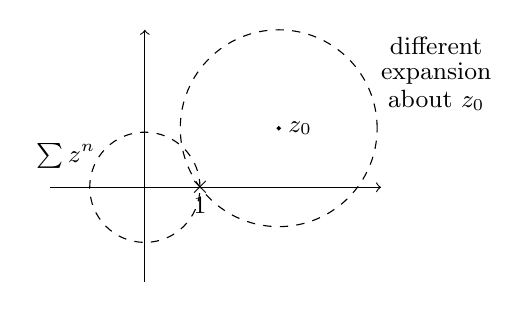
\begin{tikzpicture}
                    \draw[->] (-1.2,0)--(3,0);
                    \draw[->] (0,-1.2)--(0,2);
                    \node at (0.7,0){\small \(\times\)};
                    \node at (0.7,0)[below]{\small \(1\)};
                    \draw[dashed] (0,0) circle (0.7);
                    \node at (-1,0.4) {\small \(\sum z^n\)};
                    \node at (1.7,0.75)[right]{\small \(z_0\)};
                    \draw[fill=black] (1.7,0.75) circle (0.02);
                    \draw[dashed] (1.7,0.75) circle (1.25);
                    \node at (3.7,1.8) {\small different};
                    \node at (3.7,1.45) {\small expansion};
                    \node at (3.7,1.1) {\small about \(z_0\)};
                \end{tikzpicture}
            \end{figure}
            \item Considering \(f(z)=\sum_{n\ge 0}z^{2^n}\), one can show that \(f\) converges on \(D(0,1)\) and cannot be analytically continued to any domain in \(U\) with \(D(0,1)\subsetneq U\). We say \(\partial D(0,1)\) is the natural boundary for \(f\).
        \end{enumerate}
    \end{exs}
    \begin{cor}[Global maximum principle]
        If \(U\subseteq\CC\) is a bounded domain and \(\overline{U}\) is its closure. (\(\overline{U}=\bigcap_{K\supseteq U\,,\;K\text{ closed}}K\)). If \(f:U\to\CC\) is continuous and \(f\) is holomorphic on \(U\), then \(\abs{f}\) achieves its maximum on \(\overline{U}\setminus U\).
    \end{cor}
    \begin{proof}
        \(\overline{U}\) is closed and bounded \(\implies\abs{f}\) achieves a maximum on \(\overline{U}\). Call it \(m\). If \(\abs{f(z_0)}=m\) for some \(z_0\in U\), then local maximum principle \(\implies f(z)\equiv f(z_0)\) for \(z\in D(z_0,\epsilon)\), \(\epsilon>0\). Then by identity theorem, \(f(z)\equiv f(z_0)\) \(\forall z\in U\). \(f\) continuous on \(\overline{U}\implies f(z)=f(z_0)\) \(\forall z\in\overline{U}\), so corollary holds.\qed
    \end{proof}
    \subsection{Generalised Cauchy Integral Formula}
    Our goal is to generalise CIF to curves other than a circle.

    We have an issue, even without changing the image set of a curve, the integral might change.
    \begin{figure}[ht!]
        \centering
        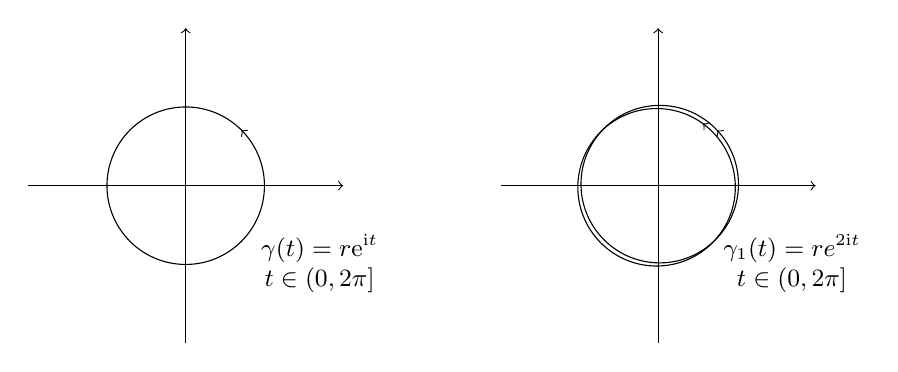
\begin{tikzpicture}
            \draw[->] (-2,0)--(2,0);
            \draw[->] (0,-2)--(0,2);
            \draw[decoration={markings, mark=at position 0.125 with {\arrow{>}}},postaction={decorate}] (0,0) circle (1);
            \node at (1.7,-0.8) {\small\(\gamma(t)=r\ee^{\ii t}\)};
            \node at (1.7,-1.2) {\small\(t\in(0,2\pi]\)};
            \draw[->] (4,0)--(8,0);
            \draw[->] (6,-2)--(6,2);
            \draw[decoration={markings, mark=at position 0.12 with {\arrow{>}}},postaction={decorate}] (6.02,0.02) circle (1);
            \draw[decoration={markings, mark=at position 0.15 with {\arrow{>}}},postaction={decorate}] (5.98,-0.02) circle (1);
            \node at (7.7,-0.8) {\small\(\gamma_1(t)=re^{2\ii t}\)};
            \node at (7.7,-1.2) {\small\(t\in(0,2\pi]\)};
        \end{tikzpicture}
    \end{figure}
    These satisfy \(\int_{\gamma_1}f=2\int_{\gamma}f\).

    We need to understand how a curve can `wind around' a point \(w\) where the integrand may not be holomorphic.

    \begin{thm}
        Let \(\gamma:[a,b]\to\CC\setminus\{w\}\) be a continuous curve. Then \(\exists\) continuous function \(\theta:[a,b]\to\RR\) such that \(\gamma(t)=w+r(t)\ee^{\ii \theta(t)}\) with \(r(t)=\abs{\gamma(t)-w}\).
    \end{thm}
    \begin{proof}
        WLOG, can assume \(w=0\). Since \(\Arg(\gamma(t))=\Arg(\frac{\gamma(t)}{\abs{\gamma(t)}})\), replace \(\gamma\) with \(\frac{\gamma}{\abs{\gamma}}\) to assume that \(\abs{\gamma(t)}=1\) \(\forall t\in[a,b]\).

        If \(\gamma\subset\CC\setminus\RR_{\le 0}\), we can use \(\Arg\) to define \(\theta\). More generally, if there is any point \(u\in S^1\) with \(\gamma(t)\ne u\) \(\forall t\in[a,b]\), then \(\gamma([a,b])\) lies in a slit plane \(\CC\setminus\{z\in\CC\mid\frac{z}{\ee^{\ii \alpha}}\in\RR_{\ge 0}\}\) for some \(\alpha\). Then \(\theta(t)=\alpha+\Arg(\frac{z}{\ee^{\ii \alpha}})\) will do.

        We subdivide \(\gamma\) so this holds on the pieces: \(\gamma\) uniformly continuous on \([a,b]\implies\exists\epsilon>0\) such that \(\forall\abs{s-t}<\epsilon\), \(\abs{\gamma(s)-\gamma(t)}<2\), i.e. \(\gamma(z)\) lies within a half plane for \(z\in[s,t]\). Subdividing \(a=a_0<a_1<\dots<a_n=b\) such that \(a_{j+1}-a_j<2\epsilon\) for all \(j\), then we have \(\abs{\gamma(t)-\gamma(\frac{a_{j+1}-a_j}{2})}<2\) \(\forall t\in[a_j,a_{j+1}]\). So \(\gamma([a_j,a_{j+1}])\) lies on a slit plane \(\forall j=0,1,\dots n-1\), and we can define continuous \(\theta_j\) on \([a_j,a_{j+1}]\) for each \(j\). For each \(a_j\), we then have
        \[\gamma(a_j)=\ee^{\ii \theta_j(a_j)}=\ee^{\ii \theta_{j-1}(a_j)}\,,\]
        and so \(\theta_j(a_j)=\theta_{j-1}(a_j)+2\pi n_j\) for some \(n_j\in\ZZ\).

        Proceeding as \(j\) varies from 1 to \(n-1\), we modify \(\theta_j\) by multiples of \(2\pi\), so that \(\theta_j\) and \(\theta_{j-1}\) agrees at \(a_j\), obtaining a continuous \(\theta:[a,b]\to\RR\) as claimed.\qed
    \end{proof}
    \begin{rem}
        Such \(\theta\) is not unique: \(\theta(t)+2n\pi\), \(n\in\ZZ\) would also work. However, if \(\theta_1\) and \(\theta_2\) are two such functions, then \(\theta_1-\theta_2\) is continuous and takes values in discrete \(2\pi\ZZ\), so is constant.
    \end{rem}
    \begin{defn}
        Let \(\gamma:[a,b]\to\CC\) be a closed curve, \(w\notin\gamma\). The \textit{winding number} or \textit{index} of \(\gamma\) about \(w\) is
        \[I(\gamma;w)\coloneqq\frac{\theta(b)-\theta(a)}{2\pi}\in\ZZ\,,\]
        where \(\theta\) is chosen such that \(\gamma(t)=w+r(t)\ee^{\ii \theta(t)}\) with \(\theta\) continuous.
    \end{defn}
    By the above remark, this is well defined.
    \begin{lem}
        Let \(\gamma:[a,b]\to\CC\) be a closed curve, \(w\notin\gamma([a,b])\). Then
        \[I(\gamma;w)=\frac{1}{2\pi \ii}\int_\gamma\frac{\dd{z}}{z-w}\,.\]
    \end{lem}
    \begin{proof}
        \(\gamma\) is piecewise \(C^1\) so \(r(t)\) and \(\theta(t)\) are continuous as well, where \(\gamma(t)=w+r(t)\ee^{\ii \theta(t)}\). We compute
        \begin{align*}
            \int_\gamma\frac{\dd{z}}{z-w}&=\int_{a}^{b}\frac{\gamma'(t)}{\gamma(t)-w}\dd{t}=\int_{a}^{b}\frac{r'(t)}{r(t)}+\ii\theta'(t)\dd{t}\\
            &=[\ln r(t)+\ii\theta(t)]_a^b\\
        \end{align*}
        Have \(r_a=r_b\) and \(\theta(b)-\theta(a)=2\pi I(\gamma;w)\).\qed
    \end{proof}
    \begin{prop}
        Let \(\gamma:[0,1]\to D(a,R)\) be a closed curve. Then \(\forall w\notin D(a,R)\), \(I(\gamma;w)=0\).
    \end{prop}
    \begin{proof}
        Consider the M\"{o}bius map \(\mu:z\mapsto\frac{z-w}{a-w}\). \(\mu(w)=0\), \(\mu(a)=1\), and since
        \[\abs{\frac{z-w}{a-w}-1}=\abs{\frac{z-a}{a-w}}\,,\]
        we see that \(D(a,\abs{a-w})\mapsto D(1,1)\). So \(\mu(D(a,R))\subseteq D(1,1)\).
        \begin{figure}[ht!]
            \centering
            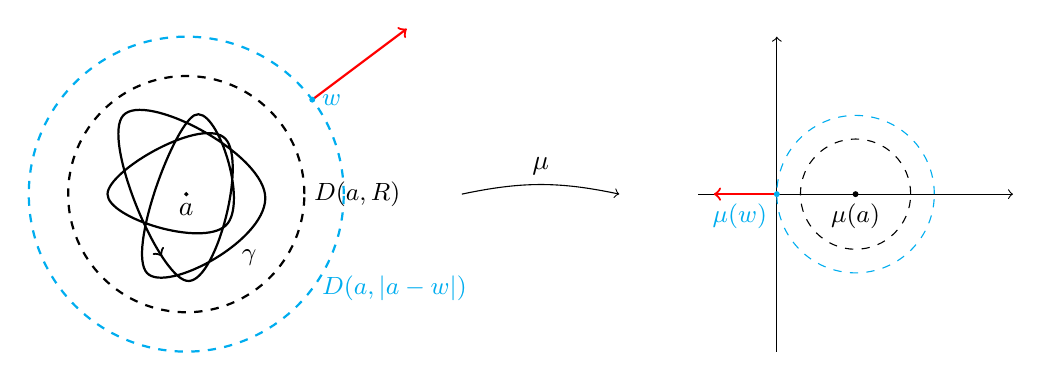
\begin{tikzpicture}
                \draw[dashed,thick] (0,0) circle (1.5);
                \draw[dashed,thick,cyan] (0,0) circle (2.0);
                \draw[fill=black] (0,0) circle (0.02)node[below]{\(a\)};
                \draw[decoration={markings, mark=at position 0.12 with {\arrow{>}}},postaction={decorate},thick] plot[smooth cycle,tension=1] coordinates {(1,0) (-0.8,1) (0,-1.1) (0.5,0.7) (-1,0) (0.5,-0.4) (0.1,1) (-0.5,-1)};
                \node at (0.8,-0.8) {\small \(\gamma\)};
                \node at (1.5,0)[right]{\small\(D(a,R)\)};
                \node[cyan] at (1.6,-1.2)[right]{\small \(D(a,\abs{a-w})\)};
                \draw[->,thick,red] (1.6,1.2)--(2.8,2.1);
                \draw[cyan,fill=cyan] (1.6,1.2) circle (0.03)node[right]{\small \(w\)};
                \draw[->] (3.5,0) to [bend left=12] node[above]{\(\mu\)}(5.5,0);
                \draw[->] (6.5,0)--(10.5,0);
                \draw[->] (7.5,-2)--(7.5,2);
                \draw[dashed,cyan] (8.5,0) circle (1);
                \draw[dashed] (8.5,0) circle (0.7);
                \draw[thick,->,red] (7.5,0)--(6.7,0);
                \draw[cyan,fill=cyan] (7.5,0) circle (0.03) node[below left]{\small \(\mu(w)\)};
                \draw[fill=black] (8.5,0) circle (0.03) node[below]{\small \(\mu(a)\)};
            \end{tikzpicture}
        \end{figure}

        On \(D(1,1)\), we have a continuous definition of the argument, and so it follows that (since \(D(a,R)\subset\CC\setminus\{z\in\CC\mid\frac{z-w}{a-w}\in\RR_{\le 0}\}\)) we have a continuous definition of \(\arg(z-w)\) on \(\gamma\). Therefore,
        \[I(\gamma;w)=\frac{\arg(\gamma(1)-w)-\arg(\gamma(0)-w)}{2\pi}=0\]
        since the curve is closed.\qed
    \end{proof}
    \begin{defn}
        Let \(U\subseteq\CC\) be open. We say that a closed curve \(\gamma\) in \(U\) is \textit{homologous to zero} if \(\forall w\notin U\), \(I(\gamma;w)=0\).
    \end{defn}
    If \(\gamma\) is homologous to zero in \(U\) for all closed curve \(\gamma\) in \(U\), then \(U\) is simply connected.
    \begin{rems}
        \begin{enumerate}[topsep=0pt,label=(\roman*)]
            \item If \(U\subseteq\CC\) is open then our two definitions of simply connected are equivalent.
            \item If \(U\subset\CC\) is connected, it is path connected.
        \end{enumerate}
    \end{rems}
    By the previous proposition, open disks are simply connected. On the other hand, any punctured disk \(D(a,R)^\times=D(a,R)\setminus\{a\}\) is not simply connected, since curves can wind around the puncture.

    \begin{thm}[Generalised Cauchy Integral Formula]
        Let \(f:U\to\CC\) be holomorphic. \(U\) is a domain and let \(\gamma\) be a closed curve in \(U\) which is homologous to zero in \(U\). Then \(\forall w\in U\setminus\gamma\),
        \[I(\gamma;w)f(w)=\frac{1}{2\pi \ii}\int_{\gamma}\frac{f(z)}{z-w}\dd{z}\,,\]
        and \(\int_{\gamma}f(z)\dd{z}=0\).
    \end{thm}
    \begin{proof}
        Notice that apply the first equality to \(g(z)=f(z)(z-w)\), we have \(\frac{1}{2\pi \ii}\int_\gamma f(z)=g(w)I(\gamma;w)=0\), so it suffices to prove the first statement. The previous lemma gives LHS
        \[I(\gamma;w)=\frac{1}{2\pi \ii}\int_{\gamma}\frac{f(w)}{z-w}\,,\]
        so we want to show that
        \[\int_\gamma\frac{f(z)-f(w)}{z-w}\dd{z}=0\]
        \(\forall w\in U\setminus\gamma\). Consider the function
        \[g(z,w)=\begin{cases}
            \frac{f(z)-f(w)}{z-w} & z\ne w\\
            f'(w) & z=w
        \end{cases}\]
        which is continuous on \(U\times U\). Want to show that
        \[\int_\gamma g(z,w)\dd{z}=0\]
        \(\forall w\in U\setminus\gamma\). Define the auxiliary function
        \[h(w)=\begin{cases}
            \int_\gamma g(\zeta,w)\dd{\zeta} & \text{for }w\in U\\
            \int_\gamma\frac{f(\zeta)}{\zeta-w}\dd{\zeta} & \text{for }w\in V=\{w\in\CC\setminus\gamma\mid I(\gamma;w)=0\}\,.
        \end{cases}\]
        If \(w\in U\cap V\), then
        \[\int_\gamma g(\zeta,w)\dd{\zeta}=\int_\gamma\frac{f(\zeta)-f(w)}{\zeta-w}\dd{\zeta}=\int_\gamma\frac{f(\zeta)}{\zeta-w}\dd{\zeta}\,,\]
        so \(h\) is well defined.

        \begin{itemize}[parsep=1em,rightmargin=30pt]
            \item \begin{clminproof}
                Claim \(\abs{h(w)}\to 0\) as \(\abs{w}\to\infty\).
            \end{clminproof}
            \begin{proof}
                Choose any \(R\gg 1\) so that \(\gamma\subset D(0,R)\), so we have that \(I(\gamma;w)=0\) \(\forall w\notin D(0,R)\) by the previous proposition. In fact, \(\gamma\) is homologous to zero in \(U\), \(I(\gamma;w)=0\) \(\forall w\notin U\), and so \(U\cup V=\CC\). \(\forall w\notin D(0,R)\), we have
            \begin{align*}
                \abs{h(w)}&=\abs{\int_\gamma\frac{f(\zeta)}{\zeta-w}\dd{\zeta}}\\
                &\le\frac{\length(\gamma)\cdot\sup_{\zeta\in\gamma}\abs{f(\zeta)}}{\abs{w}-R}\to 0\text{ as }\abs{w}\to\infty\,.
            \end{align*}\qed
            \end{proof}

            \item \begin{clminproof}
                \(h\) is holomorphic on \(U\cup V\), i.e. entire.
            \end{clminproof}
            \begin{proof}
                We need two lemmas.
                \begin{itemize}[parsep=1em,rightmargin=30pt]
                    \item \begin{leminproof}[Fubini's theorem]
                        Let \(f:[a,b]\times[c,d]\) be continuous, then
                        \[\int_a^b\left(\int_c^df(x,y)\dd{y}\right)\dd{x}=\int_{c}^{d}\left(\int_{a}^{b}f(x,y)\dd{x}\right)\dd{y}\,.\]
                    \end{leminproof}
                    \begin{proof}
                        Obviously hold if \(f\) is const., so also hold when \(f\) is a step function. Since \([a,b]\times[c,d]\) is bounded and compact, \(f\) is uniformly continuous. So \(f\) is uniformly approximated by step functions. So we can exchange limit and integral on the uniform approximation, and so the equality holds for \(f\) as well.\qed
                    \end{proof}
                    \item \begin{leminproof}
                        Let \(U\subset\CC\) be open, and \(\phi:U\times[a,b]\to\CC\) continuous with \(z\mapsto\phi(z,s)\) holomorphic on \(U\) for all \(s\in[a,b]\), then \(g(z)=\int_{a}^{b}\phi(z,s)\dd{s}\) is holomorphic on \(U\).
                    \end{leminproof}
                    \begin{proof}
                        We will use Morera's theorem. Holomorphicity is local, so WLOG, \(U\) is a unit disk. Let \(\gamma:[0,1]\to U\) be a closed curve, then by Fubini's theorem
                        \begin{align*}
                            \int_{\gamma}g(z)\dd{z}&=\int_{0}^{1}\left[\int_{a}^{b}\phi(\gamma(t),s)\dd{s}\right]\gamma'(t)\dd{t}\\
                            &=\int_{a}^{b}\left[\int_{0}^{1}\phi(\gamma(t),s)\gamma'(t)\dd{t}\right]\dd{s}\\
                            &=\int_{a}^{b}\left[\int_\gamma\phi(z,s)\dd{z}\right]\dd{s}\,.\\
                        \end{align*}
                        \(\phi(z,s)\) is holomorphic for fixed \(s\), so by Cauchy's theorem on a disk,
                        \[\int_\gamma\phi(z,s)=0\,,\]
                        and by Morera, \(g\) is holomorphic.\qed
                    \end{proof}
                \end{itemize}
                Applying this lemma with \(h(w)=\int_\gamma g(\zeta,w)\dd{\zeta}\) for \(w\in U\) (think of \(\zeta\) as the input to \(\gamma\)), we conclude that \(h\) is holomorphic as claimed.\qed 
            \end{proof}
        \end{itemize}

        Now since \(h\) is entire, it is continuous, and since \(\abs{h}\to 0\) as \(\abs{w}\to\infty\), we have \(h\) bounded. By Liouville's theorem, \(h\) is constant, so \(h\) is \(0\). Then by the definition of \(h\) and \(g\), for all \(w\in U\setminus\gamma\),
        \[ h(w)=\int_\gamma\frac{f(z)-f(w)}{z-w}\dd{z}=0\,,\]
        which is exactly what we would like to show.\qed
    \end{proof}
    \begin{cor}[Cauchy's theorem on simply connected domain]
        Let \(U\) be simply connected, \(f:U\to\CC\) holomorphic, then for any closed curve \(\gamma\subset U\), \(\int_\gamma f=0\).
    \end{cor}
    \begin{lem}
        Winding number is locally constant. If \(\gamma\) is a closed curve and \(w\notin\gamma\), then \(\exists D(w,\rho)\) such that \(\forall w'\in D(w,\rho)\), \(I(\gamma;w)=I(\gamma;w')\).
    \end{lem}
    \begin{proof}
        Choose \(r>0\) small with \(D(w,r)\subset\CC\setminus\gamma\). Take \(w<1\) and consider \(w'\in D(w,r^3)\). We have
        \begin{align*}
            \abs{I(\gamma;w)-I(\gamma;w')}&=\frac{1}{2\pi}\abs{\int_\gamma\frac{1}{z-w}-\frac{1}{z-w'}\dd{z}}\\
            &=\frac{1}{2\pi}\abs{\int_\gamma\frac{w-w'}{(z-w)(z-w')}\dd{z}}\\
            &\le\frac{1}{2\pi}\length(\gamma)\cdot\frac{r^3}{r(r-r^3)}\to 0\text{ as }r\to 0\,.
        \end{align*}
        In particular, this is \(<1\) for \(r\ll 1\) and so \(I(\gamma;w)=I(\gamma;w')\), since both of them are integers.\qed
    \end{proof}
    \subsection{Singularities and Laurent Expansions}
    \begin{thm}[Laurent expansion]
        Let \(f\) be holomorphic on an annulus \(A=\{z\in\CC\mid r<\abs{z-a}<R\}\), where \(0<r<R\le\infty\). Then
        \begin{enumerate}[topsep=0pt,label=(\roman*)]
            \item \(f\) has a unique convergent expansion on \(A\)
            \[f(z)=\sum_{n=-\infty}^{\infty}c_n(z-a)^n\]
            called \textit{Laurent expansion}.
            \item If \(r<\rho'\le\rho<R\), then the Laurent series converges uniformly on \(\{z\in\CC\mid\rho'\le\abs{z-a}\le\rho\}\).
            \item For any \(r<\rho<R\), we have
            \[c_n=\frac{1}{2\pi \ii}\int_{\partial D(a,\rho)}\frac{f(z)}{(z-a)^{n+1}}\dd{z}\,.\]
        \end{enumerate}
    \end{thm}
    \begin{proof}
        Fix \(w\in A\), and choose \(r<\rho_1<\abs{w-a}<\rho_2<R\). Define contours \(\gamma_1,\gamma_2\) as shown.
        \begin{figure}[ht!]
            \centering
            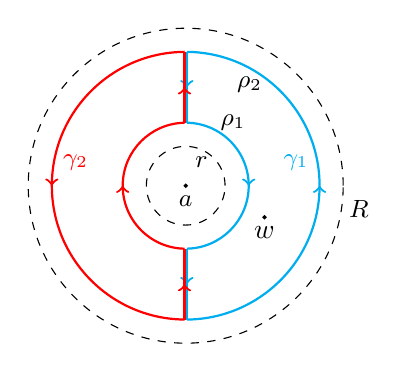
\begin{tikzpicture}
                \draw[dashed] (0,0) circle (2);
                \draw[dashed] (0,0) circle (0.5);
                \draw[fill=black] (0,0) circle (0.02) node[below]{\small \(a\)};
                \node at (0.2,0.3) {\small \(r\)};
                \node at (2.2,-0.3) {\small \(R\)};
                \draw[cyan,thick,decoration={markings, mark=at position 0.5 with {\arrow{>}}},postaction={decorate}] (0.015,-1.7)arc(-89.5:89.5:1.7);
                \draw[cyan,thick,decoration={markings, mark=at position 0.5 with {\arrow{>}}},postaction={decorate}] (0.015,1.7)--(0.015,0.8);
                \draw[cyan,thick,decoration={markings, mark=at position 0.5 with {\arrow{>}}},postaction={decorate}] (0.015,0.8)arc(88.94:-88.94:0.8);
                \draw[cyan,thick,decoration={markings, mark=at position 0.5 with {\arrow{>}}},postaction={decorate}] (0.015,-0.8)--(0.015,-1.7);
                \draw[red,thick,decoration={markings, mark=at position 0.5 with {\arrow{>}}},postaction={decorate}] (-0.015,1.7)arc(90.5:269.5:1.7);
                \draw[red,thick,decoration={markings, mark=at position 0.5 with {\arrow{>}}},postaction={decorate}] (-0.015,-1.7)--(-0.015,-0.8);
                \draw[red,thick,decoration={markings, mark=at position 0.5 with {\arrow{>}}},postaction={decorate}] (-0.015,-0.8)arc(268.94:91.06:0.8);
                \draw[red,thick,decoration={markings, mark=at position 0.5 with {\arrow{>}}},postaction={decorate}] (-0.015,0.8)--(-0.015,1.7);
                \node[cyan] at (1.4,0.3) {\small\(\gamma_1\)};
                \node[red] at (-1.4,0.3) {\small\(\gamma_2\)};
                \draw[fill=black] (1,-0.4) circle (0.02)node[below]{\(w\)};
                \node at (0.6,0.8){\small \(\rho_1\)};
                \node at (0.81,1.28){\small \(\rho_2\)};
            \end{tikzpicture}
        \end{figure}

        We have \(I(\gamma_1;w)=1\), \(I(\gamma_2;w)=0\). By generalised CIF, we have
        \begin{align*}
            f(w)&=\frac{1}{2\pi \ii}\int_{\gamma_1}\frac{f(z)}{z-w}\dd{z}\\
            &=\frac{1}{2\pi \ii}\int_{\gamma_1+\gamma_2}\frac{f(z)}{z-w}\dd{z}\\
            &=\underbrace{\frac{1}{2\pi \ii}\int_{\abs{z-a}=\rho_2}\frac{f(z)}{z-w}\dd{z}}_{I_2}\underbrace{-\frac{1}{2\pi \ii}\int_{\abs{z-a}=\rho_1}\frac{f(z)}{z-w}\dd{z}}_{I_1}\,.
        \end{align*}

        To compute \(I_2\), note that
        \[\frac{1}{z-w}=\frac{1}{(z-a)-(w-a)}=\frac{1}{z-a}\frac{1}{1-\frac{w-a}{z-a}}\,,\]
        so
        \begin{align*}
            I_2&=\frac{1}{2\pi \ii}\int_{\abs{z-a}=\rho_2}\frac{f(z)}{z-a}\sum_{n=0}^{\infty}\left(\frac{w-a}{z-a}\right)^n\dd{z}\\
            &=\sum_{n=0}^{\infty}\left(\frac{1}{2\pi \ii}\int_{\abs{z-a}=\rho_2}\frac{f(z)}{(z-a)^{n+1}}\dd{z}\right)(w-a)^n\,.
        \end{align*}
        Notice this expression of \(I_2\) converges uniformly on \(\overline{D(a,\rho')}\) for any \(\rho'< R\).

        To compute \(I_1\), we have
        \[-\frac{1}{z-w}=\frac{1/(w-a)}{1-(z-a)/(w-a)}=\sum_{m=1}^{\infty}\frac{(z-a)^{m-1}}{(w-a)^m}\,,\]
        which gives
        \[I_1=\sum_{m=1}^{\infty}\left(\frac{1}{2\pi \ii}\int_{\abs{z-a}=\rho_1}\frac{f(z)}{(z-a)^{-m+1}}\dd{z}\right)(w-a)^{-m}\,.\]
        Re-indexing with \(n=-m\), we obtain the negative power parts of Laurent expansion, proving (i) and (ii).

        To show (iii), suppose \(f(z)=\sum_{n=-\infty}^{\infty}c_n(z-a)^n\) on \(A\) and let \(r<\rho<R\). The non-negative part of the Laurent expansion converges uniformly on \(\overline{D(a,\rho)}\). Similarly, let \(u=\frac{1}{z-a}\), then the negative part of the Laurent expansion has radius of convergence \(\ge\frac{1}{r}\), i.e. converges uniformly on \(\CC\setminus D(a,\rho)\). We have uniform convergence on \(\abs{z-a}=\rho\) so
        \[\frac{1}{2\pi \ii}\int_{\partial D(a,\rho)}\frac{f(z)}{(z-a)^{m+1}}\dd{z}=\frac{1}{2\pi \ii}\sum_{n=-\infty}^{\infty}c_n\int_{\partial D(a,\rho)}(z-a)^{n-m-1}\dd{z}\,.\]
        This integral is zero unless \(n-m-1=-1\), i.e. \(n=m\), in which case it is \(2\pi \ii\), so
        \[\frac{1}{2\pi \ii}\int_{\partial D(a,\rho)}\frac{f(z)}{(z-a)^{m+1}}\dd{z}=\frac{1}{2\pi \ii}c_m\cdot 2\pi \ii=c_m\]
        as claimed.\qed
    \end{proof}
    \begin{defn}
        A point \(a\in U\) is an \textit{isolated singularity} of \(f:U\to \CC\) holomorphic if \(\exists r>0\) such that \(D(a,r)^\times\subseteq U\), i.e. \(f\) is holomorphic on a punctured neighbourhood of \(a\).
    \end{defn}
    \begin{exs}
        \begin{enumerate}[topsep=0pt,label=(\roman*)]
            \item \(a=0\), \(f(z)=\frac{\sin z}{z}\). By the identity theorem, \(\sin z=z-\frac{z^3}{3!}+\frac{z^5}{5!}+\dots\) about \(0\) converging on \(\CC\implies f(z)=1-\frac{z^2}{3!}+\frac{z^4}{5!}+\dots\) about 0. Therefore \(f\) is the restriction of a holomorphic function on \(\CC\), which takes the value \(1\) at \(0\).
            \item \(a=0\), \(g(z)=\frac{1}{z^n}\) for \(b\in\NN\) holomorphic on \(\CC^\times\) and \(g(z)\to \infty\) as \(\abs{z}\to 0\), so \(g\) cannot extend to a function holomorphic at \(0\).
            \item \(a=0\), \(h(z)=\ee^{1/z}\) on \(\CC^\times\). Recall \(\ee^{w}=w^{\Re w}\cdot \ee^{\ii \Im w}\).
            \begin{figure}[ht!]
                \centering
                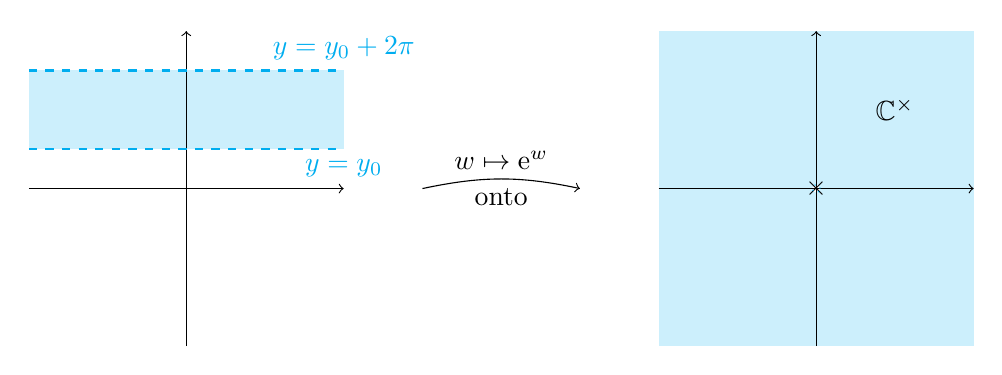
\begin{tikzpicture}
                    \fill [cyan!20] (-2,0.5) rectangle (2,1.5);
                    \draw[->] (-2,0)--(2,0);
                    \draw[->] (0,-2)--(0,2);
                    \draw [thick,dashed,cyan] (-2,0.5)--(2,0.5)node[below]{\(y=y_0\)};
                    \draw [thick,dashed,cyan] (-2,1.5)--(2,1.5)node[above]{\(y=y_0+2\pi\)};
                    \draw[->] (3,0) to [bend left=12] node[above]{\(w\mapsto \ee^w\)}node[below]{onto}(5,0);
                    \fill[cyan!20] (6,-2) rectangle (10,2);
                    \fill[white] (8,0) circle (0.05);
                    \draw[->] (6,0)--(10,0);
                    \draw[->] (8,-2)--(8,2);
                    \node at (8,0) {\(\times\)};
                    \draw[dotted,cyan] (8,0) circle (0.05);
                    \node at (9,1) {\(\CC^\times\)};
                \end{tikzpicture}
            \end{figure}

            The map \(z\mapsto \frac{1}{z}\) maps \(D(0,\epsilon)^\times\mapsto\{z\in\CC\mid\abs{z}>\frac{1}{\epsilon}\}\), which contains of horizontal strip of height \(2\pi\), so \(h(D(0,\epsilon)^\times)=\CC^\times\) no matter how small \(\epsilon\) is. Note
            \[\ee^{1/z}=\sum_{n=0}^{\infty}\frac{(1/z)^n}{n!}=\sum_{n=-\infty}^{0}\frac{1}{(-n)!}z^n\,.\]
        \end{enumerate}
    \end{exs}
    
    Let \(f\) have an isolated singularity at \(a\), with a Laurent expansion about \(a\)
    \[f(z)=\sum_{n=-\infty}^{\infty}c_n(z-a)^n\,.\]
    \begin{enumerate}[topsep=0pt,label=(\roman*)]
        \item If \(c_n=0\) \(\forall n<0\), then \(f\) is the \textit{restriction of a holomorphic function} at \(a\), and we say that \(a\) is a \textit{removable singularity} of \(f\). Example: \(f(z)=\sin z/z\) has a removable singularity at \(0\).
        \item If \(\exists k>0\) such that \(c_{-k}\ne 0\) but \(c_{-n}=0\) \(\forall n>k\). Then \((z-a)^kf(z)\) extends to a holomorphic function non-zero at \(k\). We then say that \(f\) has a \textit{pole of order \(k\)} at \(a\). Example: \(g=z^{-n}\), \(n\in\ZZ\) has a pole of order \(n\) at \(z=0\).
        \item If \(c_{-n}\ne 0\) for infinitely many \(n>0\), we say that \(f\) has an \textit{essential singularity} at \(a\). Example: \(h=\ee^{1/z}\) has an essential singularity at \(0\).
    \end{enumerate}
    \begin{prop}
        An isolated singularity \(a\) of \(f\) is removable
        \[\iff \lim_{z\to a}(z-a)f(z)=0\,.\]
    \end{prop}
    \begin{proofskip}
        \begin{itemize}[topsep=0pt]
            \item[(\(\Rightarrow\))] Trivial.
            \item[(\(\Leftarrow\))] Consider the function
            \[g(z)=\begin{cases}
                (z-a)^2f(z) & z\ne a\\
                0 & z=a\,.
            \end{cases}\]
            \[\frac{g(z)-g(a)}{z-a}=\frac{(z-a)^2f(z)}{z-a}=(z-a)f(z)\to 0\]
            as \(z\to a\), so \(g(z)\) is holomorphic at \(a\) with \(g(a)=g'(a)=0\). Therefore can write \(g(z)=\sum_{n=2}^{\infty}b_n(z-a)^n\), and we have \(f(z)=\sum_{n=0}^{\infty}b_{n+2}(z-a)^n\), so the singularity is removable.\qed
        \end{itemize}
    \end{proofskip}
    \begin{prop}
        An isolated singularity is a pole \(\iff\abs{f(z)}\to\infty\) as \(z\to a\). Moreover, the following are equivalent:
        \begin{enumerate}[topsep=0pt,label=(\roman*)]
            \item \(f\) has a pole of order \(k\) at \(z=a\).
            \item \(f(z)=(z-a)^{-k}g(z)\) for some \(g\) holomorphic and non-zero at \(a\).
            \item \(f(z)=\frac{1}{h(z)}\), where \(h\) is holomorphic at \(a\) with a zero of order \(k\) at \(a\).
        \end{enumerate}
    \end{prop}
    \begin{proof}
        (i)\(\Leftrightarrow\)(ii) by considering the Laurent expansion.

        (ii)\(\Leftrightarrow\)(iii) since \(g\) is holomorphic and non-zero at \(a\iff\frac{1}{g}\) is holomorphic and non-zero at \(a\).
        
        If \(f\) has a pole of order \(k\) at \(a\), then \(f(z)=(z-a)^{-k}g(z)\), where \(g(z)\) is holomorphic and non-zero at \(a\), so \(\abs{f(z)}=\abs{\frac{g(z)}{(z-a)^k}}\to\infty\) as \(z\to a\).
        
        Now suppose \(\abs{f(z)}\to\infty\) as \(z\to a\) at an isolated singularity \(a\). Then \(\exists\epsilon>0\) such that \(f\) is non-zero on \(D(a,\epsilon)^\times\), so \(\frac{1}{f}\) is holomorphic on \(D(a,\epsilon)^\times\).  We have \(\frac{1}{f(z)}\to 0\) as \(z\to a\), so by the previous proposition, the singularity of \(\frac{1}{f}\) at \(z=a\) is removable. Therefore, \(h=1/f\) is holomorphic at \(a\), and \(h\) has a zero of order \(k>0\) at \(a\). Write \(h(z)=(z-a)^k l(z)\), where \(l(z)\) is holomorphic and non-zero at \(a\), then
        \[f(z)=\frac{1}{(z-a)^k l(z)}=\frac{g(z)}{(z-a)^k}\]
        for some \(g\) holomorphic and non-zero at \(a\). Therefore \(f\) has a pole of order \(k\) at \(a\).\qed
    \end{proof}
    \begin{thm}[Casorati--Weierstrass theorem]
        If \(f:D(a,r)^\times\to\CC\) has an essential singularity at \(a\), then \(f\) has a dense image in \(\CC\) at any punctured neighbourhood of \(a\), i.e. \(\forall w\in\CC\), \(\epsilon>0\) and \(\forall\delta>0\), \(\exists z\in D(a,\delta)^\times\) with \(f(z)\in D(w,\epsilon)\).
    \end{thm}
    \begin{proof}
        If this does not hold and we have some \(D(a,\delta)^\times\) and some \(D(w,\epsilon)\) with \(f(z)\notin D(w,\epsilon)\) \(\forall z\in D(a,\delta)^\times\), then
        \[g(z)=\frac{1}{f(z)-w}\]
        must be holomorphic on \(D(a,\delta)^\times\), with zeros at the poles of \(f\), and bounded by \(1/\epsilon\). Therefore the singularity of \(g(z)\) at \(a\) is removable. Hence we can re-express \(f\) as
        \[f(z)=\frac{1}{g(z)}+b\,.\]
        If \(\lim_{z\to a}g(z)=0\), then \(f(z)\) has a pole at \(a\). If \(\lim_{z\to a}g(z)\) is some finite, non-zero value, then \(f(z)\) has a removable singularity at \(a\). Both contradicts the hypothesis.\qed
    \end{proof}
    There is a stronger result that is much harder to prove.
    \begin{thm}[Great Picard theorem]
        If \(f\) has an essential singularity at \(a\), then \(\exists b\in\CC\) such that \(\forall\epsilon>0\) with \(D(a,\epsilon)^\times\subseteq\text{domain of }f\), we have
        \[C\setminus\{b\}\subseteq f(D(a,\epsilon)^\times)\,.\]
    \end{thm}
    Example: \(f=\ee^{1/z}\), \(b=0\).
    \begin{rem}
        If \(f:D(a,r)^\times\to\CC\) has a pole at \(z=a\), then \(f\) extends to a continuous function \(\{D(a,r)\to\CC\cup\{\infty\}\}\), the Riemann sphere. \(f\) is then ``holomorphic in \(C_\infty\) sense'', since if we change coordinates on the image near \(a\), e.g. consider \(1/f\) near \(a\), this is holomorphic.
    \end{rem}
    \newpage
    \section{Residues}
    \subsection{Residue Theorem}
    \begin{defn}
        Let \(U\) be a domain. A function \(f\) is \textit{meromorphic} on \(U\) if \(f:D\setminus S\to\CC\) is holomorphic where \(S\) is a set of isolated singularities for \(f\) that are non-essential.
    \end{defn}
    \begin{defn}
        Let \(f:D(a,r)^\times\to\CC\) be holomorphic with Laurent expansion \(f(z)=\sum_{n=-\infty}^{\infty}c_n(z-a)^n\). The \textit{residue} of \(f\) at \(z=a\) is
        \[\Res_{z=a}f\coloneqq c_{-1}\,.\]
        The \textit{principal part} of \(f\) at \(z=a\) is \(\sum_{n=-\infty}^{-1}c_n(z-a)^n\).
    \end{defn}
    \begin{prop}
        Let \(\gamma\) be a closed curve in \(D(a,r)^\times\), then
        \[\int_{\gamma}f(z)\dd{z}=2\pi \ii I(\gamma;a)\Res_{z=a}f(z)\,.\]
    \end{prop}
    \begin{proof}
        Since the Laurent expansion \(f(z)=\sum_{n} c_n(z-a)^n\) converges uniformly on \(\gamma\), we have
        \[\int_\gamma f(z)\dd{z}=\sum_{n=-\infty}^{\infty}c_n\left[\int_{\gamma}(z-a)^n\dd{z}\right]\,.\]
        Have
        \[\int_\gamma(z-a)^n\dd{z}=\begin{cases}
            0 & n\ne -1\\
            2\pi \ii I(\gamma;a) & n=-1
        \end{cases}\]
        proving the proposition.\qed
    \end{proof}

    If \(f\) is meromorphic on a domain \(D\) and \(z=a\) is a pole of \(f\), then we have the principal part
    \[\frac{c_{-k}}{(z-a)^k}+\dots+\frac{c_{-1}}{z-a}\]
    of \(f\) at \(a\) is holomorphic on \(\CC\setminus\{a\}\). More generally, if \(\{a_1,\dots,a_m\}\subseteq\{\text{poles of }f\text{ in }D\}\), denote \(p_i(z)\) the principal part of \(f\) at \(a_i\), then
    \[g(z)\coloneqq f(z)-\sum_{i=1}^{m}p_i(z)\]
    has removable singularities at \(a_i\) for each \(i\), and is also meromorphic on \(D\).
    \begin{thm}[Residue theorem]
        Let \(f\) be meromorphic on a domain \(D\) and \(\gamma\) is a closed curve which is homologous to \(0\) in \(D\). Assume no poles of \(f\) lie in \(\gamma\), and only finitely many poles of \(f\) have \(I(\gamma;a_i)\ne 0\), call them \(\{a_1,\dots,a_m\}\), then
        \[\int_\gamma f(z)\dd{z}=2\pi \ii\sum_{i=1}^{m}I(\gamma;a_i)\Res_{z=a_i}f(z)\,.\]
    \end{thm}
    \begin{proof}
        Let \(p_i(z)\) denote the principal part of \(f\) at \(z=a_i\), and \(g(z)=f(z)-\sum_{i=1}^{\infty}p_i(z)\). Let \(D'=D\setminus\{\text{poles }a\text{ of }f\text{ with }I(\gamma;a)=0\}\). Note \(\gamma\) is homologous to zero in \(D'\), then \(g\) is holomorphic in \(D'\), so by Cauchy's theorem,
        \[\int_\gamma g(z)\dd{z}=0\,,\]
        so \(\int_\gamma f(z)\dd{z}=\sum_{i=1}^{m}\int_\gamma p_i(z)\dd{z}\). By the previous proposition, we have \(\int_\gamma p_i(z)\dd{z}\) to be
        \[2\pi \ii I(\gamma;a_i)\Res_{z=a_i}f(z)\,.\]\qed
    \end{proof}
    \begin{rems}
        \begin{enumerate}[topsep=0pt,label=(\roman*)]
            \item We've shown that \(\{z\in\CC\setminus\gamma\mid I(\gamma;z)=0\}\) is open in \(\CC\), so its complement \(\{z\in\CC\mid I(\gamma;z)\ne0\}\cup\gamma\) is closed. This set is also bounded, so by Bolzano--Weierstrass, any infinite subset has an accumulation point. Since we assume that the poles of \(f\) are isolated, there can only be finitely many of them.
            \item If \(f\) is holomorphic on \(D\), then residue theorem \(\implies\) Cauchy's theorem.
            \item Taking \(f(z)=\frac{g(z)}{z-a}\), where \(g\) is holomorphic in \(D\), then \(\Res_{z=a}f(z)=g(a)\), so residue theorem \(\implies\) CIF.
            \item We say a closed curve \(\gamma\) \textit{bounds} a domain \(U\) if
            \[I(\gamma,z)=\begin{cases}
                1 & \text{if }z\in U\\
                0 & \text{if }z\notin U\,.
            \end{cases}\]
            If \(\gamma\) is a closed curve in \(D\) bounding a domain \(U\), and if \(f\) is holomorphic in \(D\), then
            \[\int_{\gamma}f=0\text{ and }\forall w\in U\setminus\gamma\,,\; \frac{1}{2\pi \ii}\int_\gamma\frac{f(z)}{z-w}\dd{z}=f(w)\,.\]
            If \(f\) is meromorphic on \(D\) with no poles on \(\gamma\), then
            \[\int_\gamma f\dd{z}=2\pi \ii\sum_{w\text{ poles in }U}\Res_{z=w}f(z)\,.\]
            \item\textbf{(Jordan Curve Theorem)} Every simply connected (continuous) curve in the plane separates \(\CC\) into two connected components --- one bounded and one unbounded.
            
            Note that this theorem is not as trivial as it seems to be. A proof of this needs techniques from algebraic topology.
        \end{enumerate}
    \end{rems}
    \subsection{Computing Residues}
    Computing Residues:
    \begin{enumerate}[topsep=0pt,label=(\roman*)]
        \item If \(f\) has a simple pole at \(z=a\), then
        \[f(z)=\frac{c_{-1}}{z-a}+c_0+c_1(z-a)+\dots\,,\]
        so
        \[\Res_{z=a}f(z)=\lim_{z\to a}(z-a)f(z)\,.\]
        \begin{ex}
            \(f(z)=\frac{1}{1+z^2}\) at \(z=\ii\):
            \[(z-\ii)f(z)=\frac{1}{z+\ii}\to\frac{1}{2\ii}\text{ as }z\to \ii\,.\]
        \end{ex}
        \item As a special case, if \(f(z)=\frac{g(z)}{h(z)}\), where \(g(z)\) holomorphic and \(h(z)\) holomorphic with a simple zero at \(z=a\), Then
        \[(z-a)f(z)=(z-a)\frac{g(z)}{h(z)}=(z-a)\frac{g(z)}{(z-a)\tilde{h}(z)}\,,\]
        where \(\tilde{h}(z)(z-a)=h(z)\). \(\tilde{h}\) holomorphic and non-zero at \(z=a\), so
        \[\Res_{z=a}f(z)=\lim_{z\to a}\frac{g(z)}{\tilde{h}(z)}=\frac{g(a)}{h'(a)}\,.\]
        \begin{ex}
            \(f(z)=\frac{\ee^z}{1+z^2}\) at \(z=\ii\). \(\Res_{z=\ii}f(z)=\frac{\ee^\ii}{2\ii}\).
        \end{ex}
        \item If \(f(z)=\frac{g(z)}{(z-a)^k}\), \(g\) holomorphic and non-zero at \(z=a\), then
        \begin{align*}
            \Res_{z=a}f(z)&=\text{coeff. of }(z-a)^{k-1}\text{ in expansion of }g\text{ about }a\\
            &=\frac{g^{(k-1)}(a)}{(k-1)!}\,.
        \end{align*}
    \end{enumerate}
    \subsection{Real Integrals via Contour Integrals}
    \begin{ex}
        Evaluate \(\int_{0}^{\infty}\frac{1}{1+x^4}\dd{x}\).

        Notice that
        \[\int_{0}^{\infty}\frac{1}{1+x^4}\dd{x}=\frac{1}{2}\lim_{R\to\infty}\int_{0}^{R}\frac{1}{1+x^4}\dd{x}\]
        and that \(\abs{\frac{1}{1+x^4}}\) is small for large \(\abs{x}\). Define contour as shown in the figure.

        \begin{figure}[ht!]
            \centering
            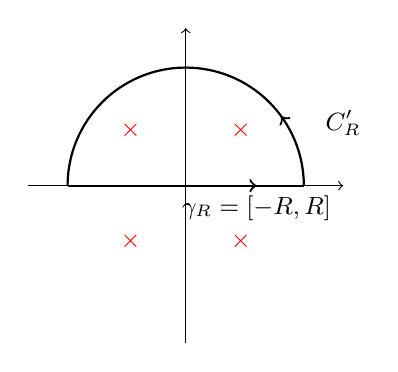
\begin{tikzpicture}
                \draw[->] (-2,0)--(2,0);
                \draw[->] (0,-2)--(0,2);
                \draw[thick,decoration={markings, mark=at position 0.2 with {\arrow{>}}},postaction={decorate}] (1.5,0) arc (0:180:1.5);
                \draw[thick,decoration={markings, mark=at position 0.8 with {\arrow{>}}},postaction={decorate}] (-1.5,0)--(1.5,0);
                \node[red] at (0.7,0.7){\small \(\times\)};
                \node[red] at (-0.7,0.7){\small \(\times\)};
                \node[red] at (0.7,-0.7){\small \(\times\)};
                \node[red] at (-0.7,-0.7){\small \(\times\)};
                \node at (2,0.8) {\small \(C_R'\)};
                \node at (0.9,0)[below]{\small \(\gamma_R=[-R,R]\)};
            \end{tikzpicture}
        \end{figure}
        
        \(f(z)=\frac{1}{1+z^4}\) is meromorphic on \(\CC\) with \(4\) simple poles at \(z=\ee^{\pi \ii/4},\ee^{3\pi \ii/4},\ee^{5\pi \ii/4},\ee^{7\pi \ii/4}\). The closed contour \(\gamma_R\cup C_R'\) winds around the first two poles (if \(R\) is large enough), and not around the last two. The residues are
        \[\Res_{z=\ee^{\pi \ii/4}}\frac{1}{1+z^4}=\frac{1}{4e^{3\pi \ii/4}}\,,\;\Res_{z=\ee^{3\pi \ii/4}}\frac{1}{1+z^4}=\frac{1}{4e^{\pi \ii/4}}\,,\]
        so the integral around the contour is
        \begin{align*}
            \lim_{R\to\infty}\int_{\gamma_R\cup C_R'}\frac{1}{1+z^4}\dd{z}&=2\pi \ii\left(\frac{1}{4e^{3\pi \ii/4}}+\frac{1}{4e^{\pi \ii}}\right)\\
            &=\frac{\pi}{\sqrt{2}}\,.
        \end{align*}
        This integral can be separated into two parts
        \[\int_{\gamma_R\cup C_R'}\frac{1}{1+z^4}\dd{z}=\underbrace{\int_{C_R'}\frac{1}{1+z^4}\dd{z}}_{I_1}+\underbrace{\int_{-R}^{R}\frac{1}{1+z^4}\dd{z}}_{I_2}\,.\]
        \(I_1\) can be parameterised as \(R \ee^{\ii \theta},\theta\in[0,\pi]\), so
        \[I_1=\int_{0}^{\pi}\frac{1}{1+R^4e^{4i\theta}}\cdot iR\ee^{\ii \theta}\dd{\theta}\]
        \[\abs{I_1}\le\frac{1}{R^4-1}\cdot\pi R\to 0\text{ as }R\to \infty\,.\]
        Hence, in the \(R\to\infty\) limit, \(I_1\) vanishes, so
        \begin{align*}
            \int_{0}^{\infty}\frac{1}{1+x^4}\dd{x}&=\frac{1}{2}\lim_{R\to\infty}\int_{\gamma_R\cup C_R'}\frac{1}{1+z^4}\dd{z}\\
            &=\frac{\pi}{2\sqrt{2}}\,.
        \end{align*}
    \end{ex}
    \begin{lem}[Jordan's lemma]
        Suppose \(f\) is holomorphic for \(\abs{z}>r\) and assume that \(zf(z)\) is bounded, then \(\forall\alpha>0\), we have
        \[\int_{C_R'}f(z)\ee^{\ii \alpha z}\dd{z}\to 0\text{ as }R\to\infty\,.\]
        Here \(C_R'\) is \([0,\pi]\to\CC\), \(C_{R}'(t)=R\ee^{\ii t}\).        
    \end{lem}
    Comment: \(\ee^{\ii \alpha z}=\ee^{\ii \alpha(x+\ii y)}=\ee^{\ii \alpha x-\alpha y}\) is small if \(\alpha y\gg 1\).
    \begin{proof}
        For \(z=R\ee^{\ii t}\), we have
        \[\abs{\ee^{\ii\alpha z}}=\ee^{-\alpha R\sin t}\]
        and so using the estimate \(\frac{\sin t}{t}\ge\frac{2}{\pi}\) on \([0,\frac{\pi}{2}]\), we have
        \[\abs{\ee^{\ii\alpha z}}\le\begin{cases}
            \ee^{-\alpha R\cdot\frac{2}{\pi}t} & \text{for }t\in[0,\frac{\pi}{2}]\\
            \ee^{-\alpha R\cdot\frac{2}{\pi}t'} & \text{for }t'=\pi-t,\text{ with }t\in[0,\frac{\pi}{2}]\,.
        \end{cases}\]
        We have some \(M\) such that \(\abs{zf(z)}\le M\) on \(C_R'\), so on the first half of \(C_R'\) (call it \(\overline{C_R'}\)), we have
        \begin{align*}
            \abs{\int_{\overline{C_R'}}f(z)\ee^{\ii \alpha z}\dd{z}}&\le \int_{0}^{\pi/2}Me^{\alpha R\frac{2}{\pi}t}\dd{t}\\
            &=M\cdot\left(-\frac{1}{\alpha R\cdot\frac{2}{\pi}}\right)\left[\ee^{-\alpha R\cdot\frac{2}{\pi}t}\right]_{t=0}^{\pi/2}\\
            &=M\cdot\left(\frac{1}{\alpha R\cdot\frac{2}{\pi}}-\frac{1}{\alpha R\cdot\frac{2}{\pi}}\ee^{-\alpha R}\right)\to 0\text{ as }R\to\infty\,.
        \end{align*}
        Similar for the second half of the curve.\qed
    \end{proof}
    \begin{ex}
        \(\int_{-\infty}^{\infty}\frac{\cos(mx)}{x^2+1}\dd{x}\), where \(m\in\RR\).

        \begin{figure}[ht!]
            \centering
            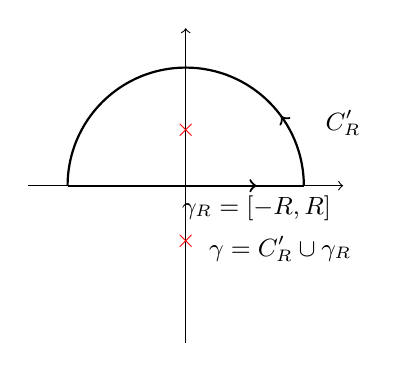
\begin{tikzpicture}
                \draw[->] (-2,0)--(2,0);
                \draw[->] (0,-2)--(0,2);
                \draw[thick,decoration={markings, mark=at position 0.2 with {\arrow{>}}},postaction={decorate}] (1.5,0) arc (0:180:1.5);
                \draw[thick,decoration={markings, mark=at position 0.8 with {\arrow{>}}},postaction={decorate}] (-1.5,0)--(1.5,0);
                \node[red] at (0,0.7){\small \(\times\)};
                \node[red] at (0,-0.7){\small \(\times\)};
                \node at (2,0.8) {\small \(C_R'\)};
                \node at (0.9,0)[below]{\small \(\gamma_R=[-R,R]\)};
                \node at (1.2,-0.8){\small \(\gamma=C_R'\cup\gamma_R\)};
            \end{tikzpicture}
        \end{figure}

        \(\cos(z)=\frac{\ee^{\ii z}+\ee^{-\ii z}}{2}\), so is large on the imaginary axis. So instead we use
        \[\cos(mx)=\Re(\exp(imx))\,,\]
        then the integral we are interested in is
        \[\Re\left(\int_{-\infty}^{\infty}\frac{\ee^{\ii mx}}{x^2+1}\dd{x}\,.\right)\]
        If \(m>0\), Jordan's lemma applies, so let us the the contour shown in the figure.

        For \(m>0\), by Jordan's lemma,
        \[\int_{C_R'}\frac{\ee^{\ii mz}}{1+z^2}\dd{z}\to 0\text{ as }R\to \infty\,.\]
        \(\frac{\ee^{\ii mz}}{1+z^2}\) has simple poles at \(z=\ii\) and \(z=-\ii\). The first pole has winding number \(1\) and the second has winding number \(0\). Have \(\Res_{z=\ii}\frac{\ee^{\ii mz}}{1+z^2}=\frac{\ee^{-m}}{2\ii}\), so 
        \begin{align*}
            \int_{-\infty}^{\infty}\frac{\cos(mz)}{z^2+1}\dd{z}&=\Re\left[\lim_{R\to\infty}\int_{\gamma}\frac{\ee^{\ii mz}}{1+z^2}\right]\\
            &=\Re\left[2\pi \ii\frac{\ee^{-m}}{2\ii}\right]=\frac{\pi}{\ee^m}\,.
        \end{align*}

        If \(m<0\), \(\cos(mx)=\cos(-mx)\), and so
        \[\int_{-\infty}^{\infty}\frac{\cos(mx)}{x^2+1}\dd{x}=\frac{\pi}{\ee^{\abs{m}}}\,.\]

        If \(m=0\), \(\int_{-\infty}^{\infty}\frac{1}{x^2+1}\dd{x}\). Using the same contour, we have
        \[\abs{\int_{C_R'}\frac{1}{z^2+1}\dd{z}}\le\frac{\pi R}{R^2+1}\to 0\text{ as }R\to\infty\,,\]
        and so \(\int_{-\infty}^{\infty}\frac{1}{z^2+1}\dd{z}=2\pi \ii\Res_{z=\ii}\frac{1}{z^2+1}=\pi\).

        Therefore, for \(m\in\RR\),
        \[\int_{-\infty}^{\infty}\frac{\cos(mx)}{x^2+1}\dd{x}=\frac{\pi}{\ee^{\abs{m}}}\,.\]        
    \end{ex}
    \begin{ex}
        Evaluate \(\int_{0}^{2\pi}\frac{1}{5+4\cos\theta}\dd{\theta}\).

        \(\cos\theta=\frac{1}{2}(\ee^{\ii \theta}+\ee^{-\ii \theta})\), so consider \(z=\ee^{\ii \theta}\) on the unit circle. Then we have \(\cos\theta=\frac{1}{2}(z+z^{-1})\) and \(\dd{z}=\ii\ee^{\ii \theta}\dd{\theta}=iz\dd{\theta}\).

        \begin{align*}
            \int_{0}^{2\pi}\frac{1}{5+4\cos\theta}\dd{\theta}&=\int_{\abs{z}=1}\frac{1}{5+2(z+z^{-1})}\frac{\dd{z}}{iz}\\
            &=-\ii\int_{\abs{z}=1}\frac{1}{2z^2+5z+2}\dd{\theta}\\
            &=2\pi\Res_{z=-\frac{1}{2}}\left(\frac{1}{2(z+\frac{1}{2})(z+2)}\right)\\
            &=\frac{2\pi}{3}\,.
        \end{align*}
    \end{ex}
    \begin{ex}
        Evaluate \(\int_{-\infty}^{\infty}\frac{\sin x}{x}\dd{x}\).

        \begin{figure}[ht!]
            \centering
            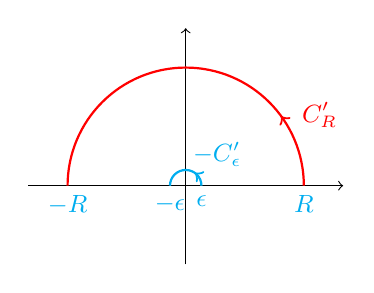
\begin{tikzpicture}
                \draw[->] (-2,0)--(2,0);
                \draw[->] (0,-1)--(0,2);
                \draw[red,thick,decoration={markings, mark=at position 0.2 with {\arrow{>}}},postaction={decorate}] (1.5,0) arc (0:180:1.5);
                \draw[cyan,thick,decoration={markings, mark=at position 0.3 with {\arrow{>}}},postaction={decorate}] (0.2,0) arc (0:180:0.2);
                \node[red] at (1.7,0.9){\small \(C_R'\)};
                \node[cyan] at (0.4,0.4){\small \(-C_\epsilon'\)};
                \node[cyan] at (0.2,0)[below]{\small\(\epsilon\)};
                \node[cyan] at (-0.2,0)[below]{\small\(-\epsilon\)};
                \node[cyan] at (1.5,0)[below]{\small\(R\)};
                \node[cyan] at (-1.5,0)[below]{\small\(-R\)};
            \end{tikzpicture}
        \end{figure}
        
        Consider
        \begin{align*}
            \frac{1}{2\ii}\int_{0}^{\infty}\frac{\ee^{\ii x}-\ee^{-\ii x}}{x}\dd{x}&=\frac{1}{2\ii}\int_{0}^{\infty}\frac{\ee^{\ii x}}{x}\dd{x}+\frac{1}{2\ii}\int_{-\infty}^{0}\frac{\ee^{\ii x}}{x}\dd{x}\\
            &=\frac{1}{2\ii}\int_{-\infty}^{\infty}\frac{\ee^{\ii x}}{x}\dd{x}\,.
        \end{align*}
        Call the closed contour shown in the figure \(\gamma_{R,\epsilon'}\). Then by Cauchy's theorem
        \[\int_{\gamma_{R},\epsilon}\frac{\ee^{\ii z}}{z}\dd{z}=0\,.\]
        By Jordan's lemma, \(\int_{C_R'}\frac{\ee^{\ii z}}{z}\dd{z}\to 0\) as \(R\to\infty\). On \(C_{\epsilon}'\), write \(z=\epsilon \ee^{\ii \theta}\), \(\theta\in[0,\pi]\), \(\dd{z}=\ii\epsilon \ee^{\ii \theta}\).
        \[\int_{C_\epsilon '}\frac{\ee^{\ii z}}{z}\dd{z}=\int_{0}^{\pi}\frac{\ee^{\ii \epsilon \ee^{\ii \theta}}}{z}\cdot iz\dd{\theta}=\int_{0}^{\pi}\ee^{\ii \epsilon \ee^{\ii \theta}}\dd{\theta}\to \ii\int_{0}^{\pi}\dd{\theta}=\pi \ii\text{ as }\epsilon\to 0\,. \]
        So
        \[-\pi \ii+\int_{-\infty}^{\infty}\frac{\ee^{\ii z}}{z}\dd{z}=0\]
        \[\implies \int_{0}^{\infty}\frac{\sin x}{x}=\frac{1}{2\ii}\int_{-\infty}^{\infty}\frac{\ee^{\ii z}}{z}\dd{z}=\frac{\pi}{2}\,.\]
    \end{ex}
    \begin{ex}
        Evaluate \(\int_{0}^{\infty}\frac{x^\alpha}{1+x^2}\dd{x}\) for \(\alpha\in(0,1)\).

        We would like to use the contour below.
        \begin{figure}[ht!]
            \centering
            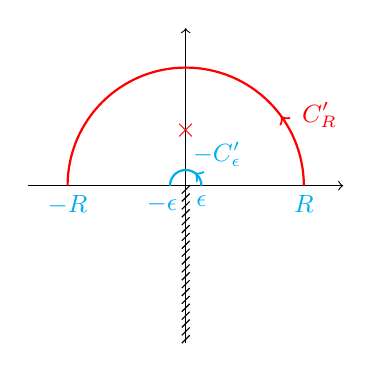
\begin{tikzpicture}
                \draw[->] (-2,0)--(2,0);
                \draw[->] (0,-2)--(0,2);
                \foreach \i in {1,...,20}{
                    \draw (-0.05,-0.1*\i)--(0.05,0.1-0.1*\i);
                }
                \draw[red,thick,decoration={markings, mark=at position 0.2 with {\arrow{>}}},postaction={decorate}] (1.5,0) arc (0:180:1.5);
                \draw[cyan,thick,decoration={markings, mark=at position 0.3 with {\arrow{>}}},postaction={decorate}] (0.2,0) arc (0:180:0.2);
                \node[red] at (1.7,0.9){\small \(C_R'\)};
                \node[cyan] at (0.4,0.4){\small \(-C_\epsilon'\)};
                \node[cyan] at (0.2,0)[below]{\small\(\epsilon\)};
                \node[cyan] at (-0.3,0)[below]{\small\(-\epsilon\)};
                \node[cyan] at (1.5,0)[below]{\small\(R\)};
                \node[cyan] at (-1.5,0)[below]{\small\(-R\)};
                \node[red] at (0,0.7){\(\times\)};
            \end{tikzpicture}
        \end{figure}

        We have
        \[z^\alpha=\exp(\alpha\log z)=\exp(\alpha\ln\abs{z}+\alpha \ii\arg(z))\,,\]
        We choose \(\arg z\in(-\frac{\pi}{2},\frac{3\pi}{2})\) to define \(\log z\) on \(\CC\setminus\{\text{negative imaginary axis}\}\), so our contour is in a domain where \(\log\) is holomorphic.

        The integral along the whole closed contour is
        \begin{align*}
            \int_{\gamma_{R,\epsilon}}\frac{z^\alpha}{1+x^2}&=2\pi \ii\Res_{z=\ii}\frac{\exp(\alpha\log z)}{(z+\ii)(z-\ii)}\\
            &=2\pi \ii\frac{\exp(\alpha\log \ii)}{2\ii}=\pi\exp\left(\frac{\pi}{2}\alpha \ii\right)\,.
        \end{align*}

        Simple estimation shows that \(\int_{C_R'}\to 0\) as \(R\to\infty\) and \(\int_{C_\epsilon'}\to 0\) as \(\epsilon\to 0\).

        Now we need to evaluate \((-x)^\alpha\) for \(x>0\) to calculate the integral on the negative real axis.
        \begin{align*}
            (-x)^\alpha&=\exp(\alpha\log(-x))\\
            &=\exp(\alpha\ln\abs{-x}+\alpha \ii\arg(-x))\\
            &=\exp(\alpha\ln x+\alpha \ii\pi)=x^\alpha\exp(\alpha \ii\pi)
        \end{align*}
        Therefore, \(\frac{(-x)^\alpha}{1+x^2}=\ee^{\alpha \ii\pi}\frac{x^\alpha}{1+x^2}\), and so
        \[\int_{-R}^{-\epsilon}\frac{z^\alpha}{1+z^2}\dd{z}=\exp(\alpha \ii\pi)\int_{\epsilon}^{R}\frac{z^\alpha}{1+z^2}\,.\]
        So we can conclude that
        \[(1+\exp(\alpha \ii\pi))\int_{0}^{\infty}\frac{x^\alpha}{1+x^2}=\pi\exp\left(\frac{\pi}{2}\alpha \ii\right)\]
        \[\int_{0}^{\infty}\frac{x^\alpha}{1+x^2}=\frac{\pi\exp(\alpha\frac{\pi}{2} \ii)}{\exp(\alpha\pi \ii)+1}\,.\]
    \end{ex}
    \begin{ex}
        Evaluate \(\int_{0}^{\infty}\frac{x^{1/3}}{(x+2)^2}\dd{x}\).
        \begin{figure}[ht!]
            \centering
            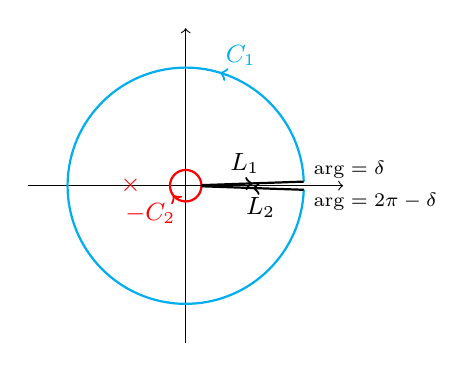
\begin{tikzpicture}
                \draw[->] (-2,0)--(2,0);
                \draw[->] (0,-2)--(0,2);
                \draw[cyan,thick,decoration={markings, mark=at position 0.2 with {\arrow{>}}},postaction={decorate}] (1.499,0.052) arc (2:358:1.5);
                \draw[red,thick,decoration={markings, mark=at position 0.4 with {\arrow{>}}},postaction={decorate}] (0.2,-0.007) arc (358:2:0.2);
                \draw[thick,decoration={markings, mark=at position 0.5 with {\arrow{>}}},postaction={decorate}] (0.2,0.007)--(1.499,0.052);
                \draw[thick,decoration={markings, mark=at position 0.5 with {\arrow{>}}},postaction={decorate}] (1.499,-0.052)--(0.2,-0.007);
                \node at (0.75,0.03)[above]{\small \(L_1\)};
                \node at (0.95,-0.03)[below]{\small \(L_2\)};
                \node[red] at (-0.45,-0.35){\small \(-C_2\)};
                \node[cyan] at (0.7,1.65){\small \(C_1\)};
                \node at (1.5,0.2)[right]{\scriptsize \(\arg = \delta\)};
                \node at (1.5,-0.2)[right]{\scriptsize \(\arg = 2\pi-\delta\)};
                \node[red] at (-0.7,0){\small \(\times\)};
            \end{tikzpicture}
        \end{figure}

        First, elementary estimates yields that the integrals on \(C_1\) and \(C_2\to 0\) as \(\epsilon\to 0\) and \(R\to\infty\).

        We choose \(\arg\in(0,2\pi)\). On \(L_1\), \(z=t\ee^{\ii \delta}\) for \(t\in(\epsilon, R)\), \(\dd{z}=\ee^{\ii \delta}\dd{t}\), so
        \[\int_{L_1}\frac{z^{1/3}}{(z+2)^2}\dd{z}=\int_{\epsilon}^{R}\frac{(t\ee^{\ii \delta})^{1/3}}{(t\ee^{\ii \delta}+2)^2}\ee^{\ii \delta}\dd{t}\,.\]
        \begin{align*}
            (t\ee^{\ii \delta})^{1/3}&=\exp\left(\frac{1}{3}\log(t\ee^{\ii \delta})\right)\\
            &=\exp\left(\frac{1}{3}\log\abs{t}+\frac{1}{3}\ii\delta\right)\to \abs{t}^{1/3}\text{ as }\delta\to 0\,,
        \end{align*}
        so \(\int_{L_1}\to\int_{\epsilon}^{R}\frac{t^{1/3}}{(t+2)^2}\dd{t}\).
        While
        \[\int_{L_2}\frac{z^{1/3}}{(z+2)^{2}}\dd{z}=\int_{\epsilon}^{R}\frac{(t\ee^{\ii (2\pi-\delta)})}{(t\ee^{\ii (2\pi-\delta)}+2)^2}\ee^{\ii (2\pi-\delta)}\dd{t}\,.\]
        \[(t\ee^{\ii(2\pi-\delta)})^{1/3}=\exp\left(\frac{1}{3}\ln\abs{t}+\frac{1}{3}\ii(2\pi-\delta)\right)\to\abs{t}^{1/3}\ee^{2\pi \ii/3}\,,\]
        so\(\int_{L_2}\to \ee^{2\pi \ii/3}\int_{\epsilon}^{R}\frac{t^{1/3}}{(t+2)^2}\dd{t}\) as \(\delta\to 0\).

        Putting all these together,
        \begin{align*}
            (1-\ee^{2\pi \ii/3})\int_{0}^{\infty}\frac{t^{1/3}}{(t+2)^2}\dd{t}&=\int_{\gamma}\frac{z^{1/3}}{(z+2)^2}\dd{z}\\
            &=2\pi \ii\Res_{z=-2}\frac{z^{1/3}}{(z+2)^2}\,.
        \end{align*}
        By the residue computation method (iii), the residue is
        \begin{align*}
            \left.\dv{}{z}\right|_{z=-2}z^{1/3}&=\left.\dv{}{z}\right|_{z=-2}\exp\left(\frac{1}{3}\log z\right)\\
            &=\left.\frac{1}{3z}\exp\left(\frac{1}{3}\log z\right)\right|_{z=-2}\,,
        \end{align*}
        so
        \[\Res_{z=-2}\frac{z^{1/3}}{(z+2)^2}=-\frac{1}{6}\sqrt[3]{2}\ee^{\pi \ii/3}\]
        and
        \[\int_{0}^{\infty}\frac{x^{1/3}}{(x+2)^2}\dd{x}=\frac{\pi\sqrt[3]{2}}{3\sqrt{3}}\,.\]
    \end{ex}
    \subsection{Rouch\'{e}'s Theorem}
    \begin{prop}
        Let \(f\) be meromorphic with a zero (or a pole) of order \(k\) at \(z=a\). Then \(\frac{f'(z)}{f(z)}\) has a simple pole at \(z=a\), with residue \(k\) (or \(-k\) for a pole).
    \end{prop}
    \begin{proof}
        If \(f\) has a zero of order \(k\) at \(z=a\), then
        \[f=(z-a)^kg(z)\,,\]
        where \(g\) is holomorphic and \(g(a)\ne 0\). So
        \[f'=k(z-a)^{k-1}g(z)+(z-a)^k g'(z)\,,\]
        and so
        \[\frac{f'(z)}{f(z)}=\frac{k}{z-a}+\frac{g'(z)}{g(z)}\,.\]
        Since \(g(a)\ne 0\),
        \[\Res_{z=a}\frac{f'}{f}=\Res_{z=a}\frac{k}{z-a}=k\]
        (respectively \(-k\) if \(a\) is a pole of order \(k\)).\qed
    \end{proof}
    This quantity \(f'/f\) is the ``logarithm derivative'' of \(f\). From example sheet 2, we know that if \(f:U\to\CC\) with \(f(U)\subseteq V\) is simply connected and omits 0, then we have a holomorphic branch of \(\log f(z)\) on \(U\), with
    \[\dv{}{z}\log f(z)=\frac{f'(z)}{f(z)}\,.\]
    \begin{thm}[Argument principle]
        Let \(\gamma\) be a closed curve which bounds a domain \(D\). Let \(f\) be a function holomorphic on an open neighbourhood of \(D\cup\gamma\). If \(f\) has no zeros or poles on \(\gamma\), then
        \[I(f\circ\gamma;0)=\frac{1}{2\pi \ii}\int_\gamma\frac{f'}{f}\dd{z}=\;\begin{pmatrix}
            \#\text{ of zeros of} \\ f\text{ in }D
        \end{pmatrix}\;-\;\begin{pmatrix}
            \#\text{ of poles of} \\ f\text{ in }D
        \end{pmatrix}\;\,,\]
        where zeros and poles are counted with their multiplicity.
    \end{thm}
    \begin{proof}
        We have
        \[I(f\circ\gamma;0)=\frac{1}{2\pi \ii}\int_{f\circ\gamma}\frac{\dd{w}}{w}=\frac{1}{2\pi \ii}\frac{f'(z)}{f(z)}\dd{z}\]
        by letting \(w=f(z)\). By residue theorem,
        \[I(f\circ\gamma;0)=\sum_{\alpha\text{ poles of }f'/f\text{ in }D}\Res_{z=\alpha}\frac{f'}{f}\,.\]
        By previous proposition, this equals to \((\#\text{ of zeros of }f\text{ in }D)-(\#\text{ of poles of }f\text{ in }D)\), counting multiplicities.\qed
    \end{proof}
    \begin{rems}
        \begin{enumerate}[topsep=0pt,label=(\roman*)]
            \item The argument principle says that
            \[2\pi[(\#\text{ zeros of }f\text{ in }D)-(\#\text{ poles of }f\text{ in }D)]\]
            is tracking the change of \(\arg f(z)\) as \(z\) travels along \(\gamma\).
            \item If interested in solving \(f(z)=c\) for some \(c\in\CC\). Let \(g(z)=f(z)-c\), then
            \begin{align*}
                I(f\circ\gamma,c)&=\frac{1}{2\pi \ii}\int_{f\circ\gamma}\frac{\dd{w}}{w-c}=\frac{1}{2\pi \ii}\int_\gamma\frac{g'(z)}{g(z)}\dd{z}\\
                &=(\#\text{ zeros of }g\text{ in }D)-(\#\text{ poles of }g\text{ in }D)\\
                &=(\#\text{ preimages of }c\text{ in }D\text{ for }f)-(\#\text{ poles of }f\text{ in }D)\,.\\
            \end{align*}
        \end{enumerate}
    \end{rems}
    \begin{defn}
        If \(f\) is holomorphic and non-constant near \(z=a\), then the \textit{local degree} (\textit{multiplicity}) of \(f\) at \(a\) is
        \[\Deg_{z=a}f(z)\coloneqq\text{the order of the zero of }f(z)-f(a)\text{ at }z=a\,.\]
    \end{defn}
    Here we have
    \[f(z)-f(a)=(z-a)^kg(z)\,,\]
    where \(g(z)\) is holomorphic and non-zero at \(a\). \(z=a\) is an isolated zero of \(f(z)-f(a)\), so \(\exists\epsilon>0\) such that \(D(a,\epsilon)^\times\) does not contain any preimage of \(f(a)\). So for sufficiently small \(\epsilon>0\), the circle \(\gamma\) of radius \(\epsilon\) about \(a\) gives
    \begin{align*}
        I(f\circ\gamma;f(a))=&\quad(\#\text{ zeros in }D(a,\epsilon)\text{ of }f(z)-f(a))\\
        &-(\#\text{ poles in }D(a,\epsilon)\text{ of }f(z)-f(a))\,.
    \end{align*}
    What if we move slightly away from \(f(a)\)?
    
    Consider the local behaviour of \(f(z)=z^k\) at \(z=0\), \(k>0\), we have \(\Deg_{z=0}f(z)=k\).
    \begin{figure}[ht!]
        \centering
        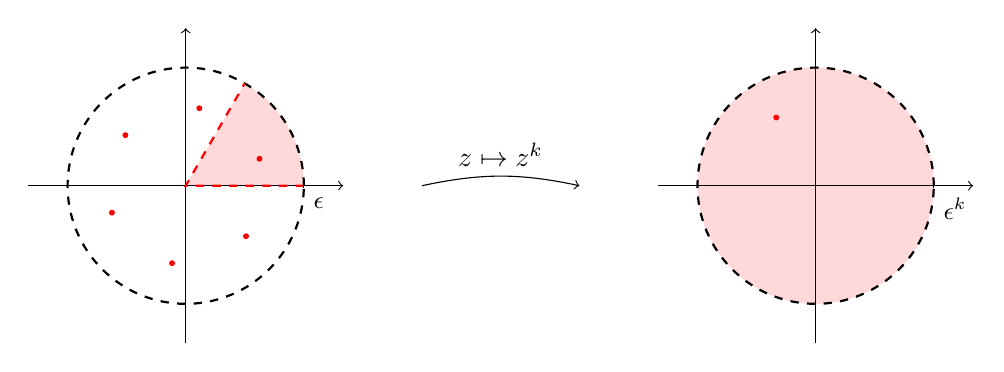
\begin{tikzpicture}
            \fill[red!15] (1.5,0) arc (0:60:1.5);
            \fill[red!15] (1.5,0)--(0,0)--(0.75,1.3);
            \draw[->] (-2,0)--(2,0);
            \draw[->] (0,-2)--(0,2);
            \draw[thick,dashed] (0,0) circle (1.5);
            \draw[thick,dashed,red] (1.5,0)--(0,0)--(0.75,1.3);
            \draw (1.5,0.03)--(1.5,-0.03)node[below right]{\small\(\epsilon\)};
            \draw[red,fill=red] (0.937,0.342) circle (0.03);
            \draw[red,fill=red] (0.173,0.984) circle (0.03);
            \draw[red,fill=red] (-0.766,0.642) circle (0.03);
            \draw[red,fill=red] (-0.937,-0.342) circle (0.03);
            \draw[red,fill=red] (-0.173,-0.984) circle (0.03);
            \draw[red,fill=red] (0.766,-0.642) circle (0.03);
            
            \draw[->] (3,0) to [bend left=12] node[above]{\(z\mapsto z^k\)}(5,0);

            \fill[red!15] (8,0) circle (1.5);
            \draw[->] (6,0)--(10,0);
            \draw[->] (8,-2)--(8,2);
            \draw[thick,dashed] (8,0) circle (1.5);
            \draw (9.5,0.03)--(9.5,-0.03)node[below right]{\small\(\epsilon^k\)};
            \draw[red,fill=red] (7.5,0.866) circle (0.03);
        \end{tikzpicture}
    \end{figure}
    
    For all \(w\in D(0,\epsilon^k)^*\), we have exactly \(k\) simple preimages of \(w\) in \(D(0,\epsilon)^\times\).

    \begin{thm}[Local degree theorem]
        Let \(f:D(a,R)\to\CC\) be holomorphic and non-constant with local degree \(k>0\) at \(z=a\). Then for \(r\) sufficiently small, \(\exists\epsilon>0\) such that \(0<\abs{w-f(a)}<\epsilon\implies w=f(z)\) has \(k\) simple solutions in \(D(a,r)\).
    \end{thm}
    \begin{proof}
        Find \(r>0\) such that \(f(z)-f(a)\) is non-zero and \(f'(z)\ne 0\) on \(\overline{D(a,r)}\setminus\{a\}\). Then \(f\circ\gamma\) does not contain \(f(a)\), so \(\exists\epsilon>0\) such that \(D(f(a),\epsilon)\cap(f\circ\gamma)=\varnothing\), where \(\gamma\) is the circle of radius \(r\) about \(a\).

        \begin{figure}[ht!]
            \centering
            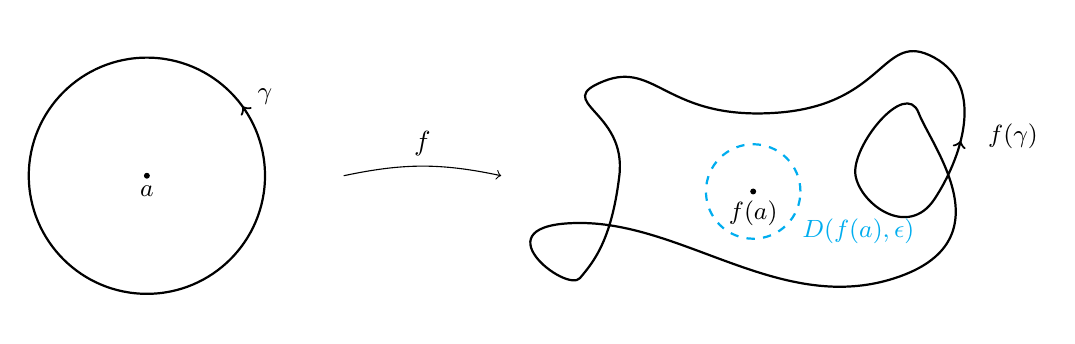
\begin{tikzpicture}
                \draw[fill=black] (0,0) circle (0.03)node[below]{\small\(a\)};
                \draw[thick,decoration={markings, mark=at position 0.1 with {\arrow{>}}},postaction={decorate}] (0,0) circle (1.5);
                \node at (1.5,1){\small\(\gamma\)};

                \draw[->] (2.5,0) to [bend left=12] node[above]{\(f\)}(4.5,0);

                \draw[thick,decoration={markings, mark=at position 0.58 with {\arrow{>}}},postaction={decorate}] plot[smooth cycle, tension=1.2] coordinates {(6,0) (5.5,-1.3) (5.5,-0.6) (9.5,-1.3) (9.8,0.8) (9,0) (10,-0.3) (10,1.5) (8,0.8) (5.8,1.2)};
                \node at (11,0.5) {\small \(f(\gamma)\)};
                \draw[fill=black] (7.7,-0.2) circle (0.03) node[below]{\small \(f(a)\)};
                \draw[thick,cyan,dashed] (7.7,-0.2) circle (0.6);
                \node[cyan] at (8.2,-0.7)[right]{\small\(D(f(a),\epsilon)\)};
            \end{tikzpicture}
        \end{figure}

        Then for \(w\in D(f(a),\epsilon)\),
        \[I(f\circ\gamma;w)=I(f\circ\gamma;f(a))\,.\]
        We have
        \begin{align*}
            I(f\circ\gamma;w)&=(\#\text{ zeros of }f(z)-w\text{ of }D(a,r))\,,\\
            I(f\circ\gamma;f(a))&=(\#\text{ zeros of }f(z)-f(a)\text{ of }D(a,r))\\
            &=\Deg_{z=a}f(z)=k\,,
        \end{align*}
        so \(w\) has \(k\) pre-images under \(f\) in \(D(a,r)\), all of which are simple since \(f'(z)\ne 0\) in \(\overline{D(a,r)}\setminus\{a\}\).\qed
    \end{proof}
    \begin{cor}[Open mapping theorem]
        Holomorphic functions are \textit{open maps} that sends open sets to open sets.
    \end{cor}
    \begin{proof}
        It suffices to prove that if \(f:U\to\CC\), then \(\forall a\in U\) and \(r>0\) sufficiently small, we can find \(\epsilon>0\) such that \(D(f(a),\epsilon)\subset f(D(a,r))\). This is immediately true by the local degree theorem, since \(\forall w\in D(f(a),\epsilon)\), we are guaranteed to have \(\Deg_{z=a}f(z)>0\) preimages of \(w\) in \(D(a,r)\).\qed
    \end{proof}
    \begin{thm}[Rouch\'{e}'s theorem]
        Let \(\gamma\) bound a domain \(D\), \(f,g\) holomorphic on a neighbourhood of \(D\cup\gamma\). If \(\abs{f(z)}>\abs{g(z)}\) \(\forall z\in\gamma\), then \(f\) and \(f+g\) have the same number of zeros in \(D\).
    \end{thm}
    \begin{proof}
        Define \(h(z)=\frac{f(z)+g(z)}{f(z)}=1+\frac{g(z)}{f(z)}\). Then \(h\) is meromorphic on a neighbourhood of \(D\cup\gamma\). Since \(\abs{f(z)}>\abs{g(z)}\) on \(\gamma\), neither \(f\) nor \(f+g\) is \(0\) on \(\gamma\), so \(h\) has no zeros or poles on \(\gamma\). By argument principle, \# zeros of \(f+g\) on \(D-\#\) zeros of \(f\) in \(D=I(h\circ\gamma;0)\). By hypothesis, \(h\circ\gamma\subset D(1,1)\), so \(I(h\circ\gamma;0)=0\).\qed
    \end{proof}
    \begin{rem}
        This is also known as the dog-walking theorem. If a person were to walk a dog on a leash around and around a tree, such that the distance between the person and the tree is always greater than the length of the leash, then the person and the dog go around the tree the same number of times.
    \end{rem}
    \begin{ex}
        Rouch\'{e}'s theorem \(\implies\) open mapping theorem.

        Suppose \(f:D\to\CC\) holomorphic and non-constant on a domain \(D\). For \(a\in D\), choose \(r>0\) such that \(\overline{D(a,r)^\times}\) has no zeros of \(f(z)-f(a)\). If \(\gamma\) is in the boundary \(\abs{z-a}=r\), then have \(0<\epsilon<\min_{z\in\gamma}\abs{f(z)-f(a)}\). Then for \(w\in D(f(a),\epsilon)\),
        \[f(z)-w=f(a)-w+f(z)-f(a)\,,\]
        so we have
        \[\abs{f(z)-w}<\epsilon+\abs{f(z)-f(a)}\]
        for all \(z\in\gamma\). By Rouch\'{e}'s theorem, \(f(z)-w\) and \(f(z)-f(a)\) have the same number of zeros inside \(\gamma\). Since we now that we have one zero or order \(k\) of \(f(z)-f(a)\) inside \(\gamma\) at \(z=a\), we also have \(k\) zeros of \(f(z)-w\), i.e. \(w\) has a preimage under \(f\) in \(D(a,r)\). So \(D(f(a),\epsilon)\subseteq f(a)\) and so \(f\) is an open map. 
    \end{ex}

    \newpage
    \section{Non-examinable Fun}
    \subsection{Homotopy}
    \begin{defn}
        Given a pair of piecewise-\(C^1\)-smooth closed paths \(\phi,\psi:[0,1]\to U\), we say \(\psi\) is an elementary deformation of \(\phi\) if there exists convex open sets \(C_1,\dots,C_n\subseteq U\) and a division of the interval \(0=x_0<x_1<\dots<x_n=1\) such that on \([x_{i-1},x_i]\), both \(\phi(t)\) and \(\psi(t)\) belong to \(C_i\).
    \end{defn}
    \begin{figure}[ht!]
        \centering
        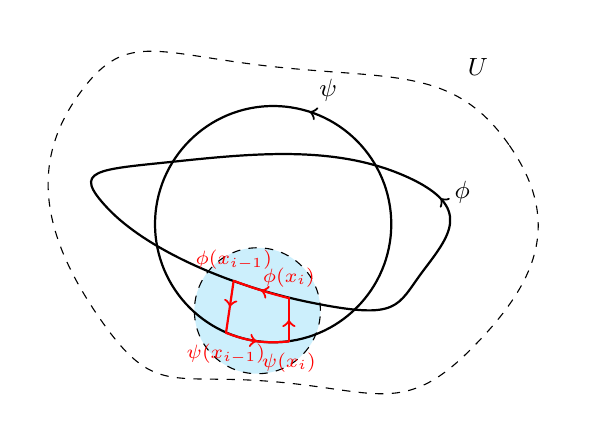
\begin{tikzpicture}
            \draw[dashed] plot[smooth cycle, tension=1] coordinates {(0,2) (3,1) (2.5,-1.6) (0,-2) (-2.2,-1.2) (-2.5,1.6)};
            \node at (2.6,2){\small \(U\)};
            \draw[dashed,fill=cyan!20] (-0.2,-1.1) circle (0.8);
            \draw[thick,decoration={markings, mark=at position 0.1 with {\arrow{>}}},postaction={decorate}] plot [smooth cycle, tension=1] coordinates {(0.5,-1) (1.9,-0.6) (1.7,0.6) (-1.2,0.8) (-2.1,0.2)};
            \node at (2.4,0.4) {\small \(\phi\)};
            \node at (0.7,1.7) {\small \(\psi\)};
            \draw[thick,decoration={markings, mark=at position 0.2 with {\arrow{>}}},postaction={decorate}] (0,0) circle (1.5);
            \draw[thick,red,decoration={markings, mark=at position 0.5 with {\arrow{>}}},postaction={decorate}] (-0.5,-0.71)node[above]{\scriptsize\(\phi(x_{i-1})\)}--(-0.6,-1.39)node[below]{\scriptsize\(\psi(x_{i-1})\)};
            \draw[thick,red,decoration={markings, mark=at position 0.5 with {\arrow{>}}},postaction={decorate}] (0.2,-1.5)node[below]{\scriptsize\(\psi(x_{i})\)}--(0.2,-0.93)node[above]{\scriptsize\(\phi(x_{i})\)};
            \draw[thick,red,decoration={markings, mark=at position 0.5 with {\arrow{>}}},postaction={decorate}] (0.2,-0.94) to [bend left=3] (-0.5,-0.72);
            \draw[thick,red,decoration={markings, mark=at position 0.5 with {\arrow{>}}},postaction={decorate}] (-0.6,-1.38) to [bend right=13] (0.2,-1.49);
        \end{tikzpicture}
    \end{figure}
    This allows us to deform a curve in a domain. If \(f\) is holomorphic on \(U\), then the integral along the red closed curve is zero. Therefore we have
    \[\int_\phi f(z)\dd{z}=\int_\psi f(z)\dd{z}\,.\]

    However, this is a rather unnatural definition, since we have to make reference to this arbitrarily constructed dissection of \([a,b]\) and convex sets \(C_i\). Moreover, this definition fails to be transitive (e.g. on \(\RR\setminus\{0\}\), rotating a circle about the center by, say, \(\pi/10\) is elementary, but rotating by \(\pi\) is not). Yet, this definition was cooked up just so that it immediately follows that elementary deformations preserve integrals of holomorphic functions around the loop.

    The idea now is to define a more general and natural notion of deforming a curve.

    \begin{defn}
        Let \(U\subseteq\CC\) be a domain, and let \(\phi,\psi:[a,b]\to U\) be piecewise-\(C^1\)-smooth closed contours. A \textit{homotopy} from \(\phi\) to \(\psi\) is a continuous map \(F:[0,1]\times[a,b]\to U\) such that
        \[F(0,t)=\phi(t)\,,\; F(1,t)=\psi(t)\,,\]
        and moreover, for all \(s\in[0,1]\), the map \(t\mapsto F(s,t)\) viewed as a map \([a,b]\to U\) is closed and piecewise-\(C^1\)-smooth. 
    \end{defn}
    We can imagine this as a process of continuously deforming the path \(\phi\) to \(\psi\), with a path \(F(s,\ \cdot \ )\) at each point in time \(s\in[0,1]\).
    \begin{prop}
        Let \(\phi,\psi:[a,b]\to U\) be homotopic contours in a domain \(U\). Then there exists some \(\phi=\phi_0,\phi_1,\dots,\phi_N=\psi\) such that each \(\phi_j\) is piecewise-\(C^1\) contour and \(\phi_{i+1}\) is obtained from \(\phi_i\) by elementary deformation.
    \end{prop}
    \begin{proof}
        Let \(F:[0,1]\times[a,b]\to U\) be a homotopy from \(\phi\) to \(\psi\). Since the image of \(F\) is compact and \(U\) is open, there exists some \(\epsilon>0\) such that \(D(F(s,t),\epsilon)\subseteq U\) for all \((s,t)\in[0,1]\times[a,b]\). Since \(F\) is uniformly continuous, there is some \(\delta\) such that \(\norm{(s,t)-(s',t')}<\delta\implies\abs{F(s,t)-F(s',t')}<\epsilon\).

        Now we pick \(n\in\NN\) such that \(\frac{1+(b-a)}{n}<\delta\) and let
        \begin{align*}
            x_j&=a+(b-a)\frac{j}{n}\\
            \phi_i(t)&=F\left(\frac{i}{n},t\right)\\
            C_{ij}&=D\left(F\left(\frac{i}{n},x_j\right),\epsilon\right)\,.
        \end{align*}
        Then \(C_{ij}\) is clearly convex. These definitions are cooked up precisely so that if \(s\in(\frac{i-1}{n},\frac{i}{n})\) and \(t\in[x_{j-1},x_j]\), then \(F(s,t)\in C_{ij}\). So the result follows.\qed
    \end{proof}
    \begin{cor}
        Let \(U\) be a domain, \(f:U\to\CC\) be holomorphic, and \(\gamma_1,\gamma_2\) be homotopic contours in \(U\), then
        \[\int_{\gamma_1}f(z)\dd{z}=\int_{\gamma_2}f(z)\dd{z}\,.\]
    \end{cor}

    This means the integral around any path depends only on the homotopy class of the path, and not the actual path itself.

    We can now use this to upgrade our Cauchy's theorem to allow arbitrary simply connected domains. The theorem will become immediate if we adopt the following alternative definition of a simply connected domain.

    \begin{defn}
        A domain \(U\) is \textit{simply connected} if every contour is homotopic to a constant path.
    \end{defn}
    This is in fact equivalent to our earlier definition that every continuous map \(S^1\to U\) can be extended to a continuous map \(D^2\to U\). This is almost immediately obvious, except that our old definition only required the map to be continuous, while the new definition only works with piecewise-\(C^1\)-paths. We will need something that allows us to approximate any continuous curve with a piecewise-\(C^1\)-smooth one, but we shall not do that here. Instead, we will just forget about the old definition and stick to the new one.

    Then we immediately have the following corollary
    \begin{cor}[Cauchy's theorem for simply connected domains]
        Let \(U\) be a simply connected domain, and let \(f:U\to\CC\) be holomorphic. For any contour \(\gamma\) in \(U\),
        \[\int_{\gamma}f(z)\dd{z}=0\,.\]
    \end{cor}
    \begin{proof}
        By definition of simply-connected, \(\gamma\) is homotopic to the constant path, and it is easy to see the integral along a constant path is zero.\qed
    \end{proof}
    We arrived at this result in a much simpler way.

    \subsection{Uniform Limits of Holomorphic Functions}
    \begin{defn}
        Let \(U\subseteq\CC\) be open, and \(f_n:U\to\CC\) a sequence of functions. We say \(f_n\to f\) \textit{locally uniformly} on \(U\) if \(\forall a\in U\), \(\exists D(a,r)\subseteq U\) such that \(f_n\to f\) uniformly on \(D(a,r)\).
    \end{defn}
    \begin{ex}
        \(f_n(z)=z^n\) on \(D(0,1)\). We have \(f_n\to 0\) pointwise, and the convergence is locally uniform. For any \(\abs{a}<1\), consider \(D(0,\abs{a}+\frac{1-\abs{a}}{2})\). We have uniform convergence on \(\overline{D(0,\abs{a}+\frac{1-\abs{a}}{2})}\) and so in particular on \(D(a,\frac{1-\abs{a}}{2})\). Note however for any \(\epsilon>0\), we have
        \[\abs{f_n(z)}\ge\epsilon\iff\abs{z^n}\ge\epsilon\iff\abs{z}\ge\epsilon^{1/n}\,,\]
        so we cannot have uniform convergence on \(D(0,1)\).
    \end{ex}
    \begin{prop}
        \(\{f_n\}:U\to\CC\) locally uniformly convergent on \(U\iff\) on any compact subset \(K\) of \(U\), \(f_n|_{K}\) converges uniformly.
    \end{prop}
    Recall from Analysis and Topology: \(K\subseteq\CC\) compact \(\iff\) \(K\) is closed and bounded \(\iff\) every open cover of \(K\) has a finite subcover.
    \begin{proof}
        \begin{itemize}
			\item[(\(\Rightarrow\))] If \(f_n\to f\) locally uniformly on \(U\) and suppose \(K\) is compact. For each \(a\in K\), \(\exists r_a>0\) such that \(f_n\to f\) uniformly on \(D(a,r_a)\). \(\bigcup_{a\in K}D(a,r_a)\) is an open cover of \(K\), so exists a finite subcover: \(K\subseteq \bigcup_{i=1}^{l} D(a_i,r_{a_i})\). \(\forall\epsilon>0\) and \(i=1,2,\dots,l\), \(\exists N_i\) such that \(n>N_i\implies\abs{f_n(z)-f(z)}<\epsilon\) for all \(z\in D(a_i,r_{a_i})\), so \(N=\max_{1\le i\le l}N_i\) gives \(\abs{f_n(z)-f(z)}<\epsilon\) for all \(z\in K\) and \(n>N\), so \(f_n\to f\) uniformly on \(K\). 
			\item[(\(\Leftarrow\))] If \(f_n\to f\) uniformly on any compact subset, then for \(a\in U\), find \(D(a,r)\subseteq U\), then \(\overline{D(a,\frac{r}{2})}\subseteq U\) so \(f_n\to f\) uniformly on \(\overline{D(a,\frac{r}{2})}\) and so on \(D(a,\frac{r}{2})\).\qed
		\end{itemize}
    \end{proof}\
    \begin{thm}
        Let \(\{f_n\}\) be a sequence of holomorphic functions on a domain \(U\), converging locally uniformly to \(f\) in \(U\), then \(f\) is holomorphic and \(f'_n\to f'\) locally uniformly.
    \end{thm}
    \begin{proof}
        Fix \(a\in U\) and \(D(a,r)\subset U\), and so \(f_n\to f\) uniformly on \(\overline{D(a,r)}\). We have
        \[\abs{f(z)-f(w)}=\abs{f(z)-f_n(z)+f_n(z)-f_n(w)+f_n(w)-f(w)}\]
        for \(z,w\in\overline{D(a,r)}\), so \(f\) is continuous on \(\overline{D(a,r)}\). Given any closed curve \(\gamma\) in \(D(a,r)\), we have
        \[\int_\gamma f=\lim_{n\to\infty}\int_\gamma f_n=0\]
        by Cauchy's theorem, so by Morera's theorem, \(f\) is holomorphic on \(D(a,r)\). So \(f\) is holomorphic on \(U\).

        By CIF, we have
        \[\abs{f'(w)-f_n'(w)}=\frac{1}{2\pi}\abs{\int_{\abs{z-a}=r}\frac{f(z)-f_n(z)}{(z-w)^2}\dd{z}}\,.\]
        If \(\abs{w-a}\le\frac{r}{2}\), then we have
        \[\abs{f'(w)-f_n'(w)}\le\frac{1}{2\pi}\cdot 2\pi r\cdot\frac{1}{(r/2)^2}\cdot\sup_{\abs{z-a}=r}\abs{f(z)-f_n(z)}\to 0\text{ as }n\to\infty\]
        by uniform convergence, so \(f_n'\to f'\) as \(n\to\infty\).\qed
    \end{proof}
    \begin{rem}
        There do exist counterexamples if we do not assume locally uniform convergence, using Runge's theorem (see Topics in Analysis). 
    \end{rem}
    \begin{prop}
        Let \(\{f_n\}\) be a sequence of holomorphic functions on a domain \(U\), \(f_n\to f\) locally uniformly on \(U\). If each \(f_n\) is injective on \(U\), then \(f\) is either injective on \(U\) or constant.
    \end{prop}
    \begin{proof}
        Suppose \(f\) is non-constant on \(U\) but \(\exists z_1\ne z_2\in U\) such that \(f(z_1)=f(z_2)=a\). \(U\) is a domain so \(\exists\) path from \(z_1\) to \(z_2\). We can find open neighbourhood of that path which is still contained in \(U\). Construct a curve \(\gamma\) that winds one around \(z_1\) and once around \(z_2\). Claim I can choose \(\gamma\) so that \(f(z)\ne a\) \(\forall z\in\gamma\). This holds since \(f\) is non constant so takes the value \(a\) at only finitely many points inside \(\gamma\) and the domain it bounds. By uniform convergence, the same is true for \(f_n\), \(n\gg 1\). So by argument principle,
        \[1\ge \frac{1}{2\pi \ii}\int_\gamma\frac{f'_n(z)}{f_n(z)-a}\dd{z}\to\frac{1}{2\pi \ii}\frac{f(z)}{f(z)-a}\dd{z}\ge 2\,.\]
        Contradiction.\qed
    \end{proof}
    \subsection{Montel's Theorem}
    \begin{defn}
        A family \(\mathcal{F}=\{f_i\}_{i\in I}\) of holomorphic functions on a domain \(U\) is \textit{normal} if every sequence \(\{f_(n)\}_{n\in\NN}\subseteq\mathcal{F}\) has some locally uniformly convergent subsequence.
    \end{defn}
    Note that we interpret ``within \(\epsilon\) of \(\infty\)'' as ``outside of \(\overline{D(0,\frac{1}{\epsilon})}\)''.
    \begin{ex}
        \(\mathcal{F}=\{z^n\mid n\in\NN\}\) is a normal family on \(\DD\) and on \(\CC_\infty\setminus\overline{D}\), with convergence to \(\equiv 0\) on \(\DD\), and to \(\equiv\infty\) on \(\CC_\infty\setminus\DD\).
    \end{ex}
    \begin{thm}[Montel's theorem]
        If \(\exists a,b,c\in\CC_\infty\) distinct with \(\forall f\in\mathcal{F}\), \(f(U)\cap\{a,b,c\}=\varnothing\), then \(\mathcal{F}\) is a normal family.
    \end{thm}
    \begin{app}
        \textbf{(Riemann mapping theorem)} Suppose \(\Omega\subsetneq\CC\) is a simply connected proper subdomain of \(\CC\), \(z_0\in\Omega\), then \(\exists\) conformal isomorphism \(f:\Omega\to\DD\) such that \(f(z_0)=0\) and \(f'(z_0)>0\).
        \begin{proof}
            Consider
            \[\mathcal{F}=\{f:\Omega\to\DD\text{ holomorphic, injective, }f(z_0)\ne 0\}\,.\]
            Proof outline:
            \begin{enumerate}[topsep=0pt]
                \item \(\mathcal{F}\ne\varnothing\).
                \item \(\exists f\in\mathcal{F}\) which maximises \(\abs{f'(z_0)}\) for functions in \(\mathcal{F}\).
                \item This \(f\) is surjective.
            \end{enumerate}
            \begin{figure}[ht!]
                \centering
                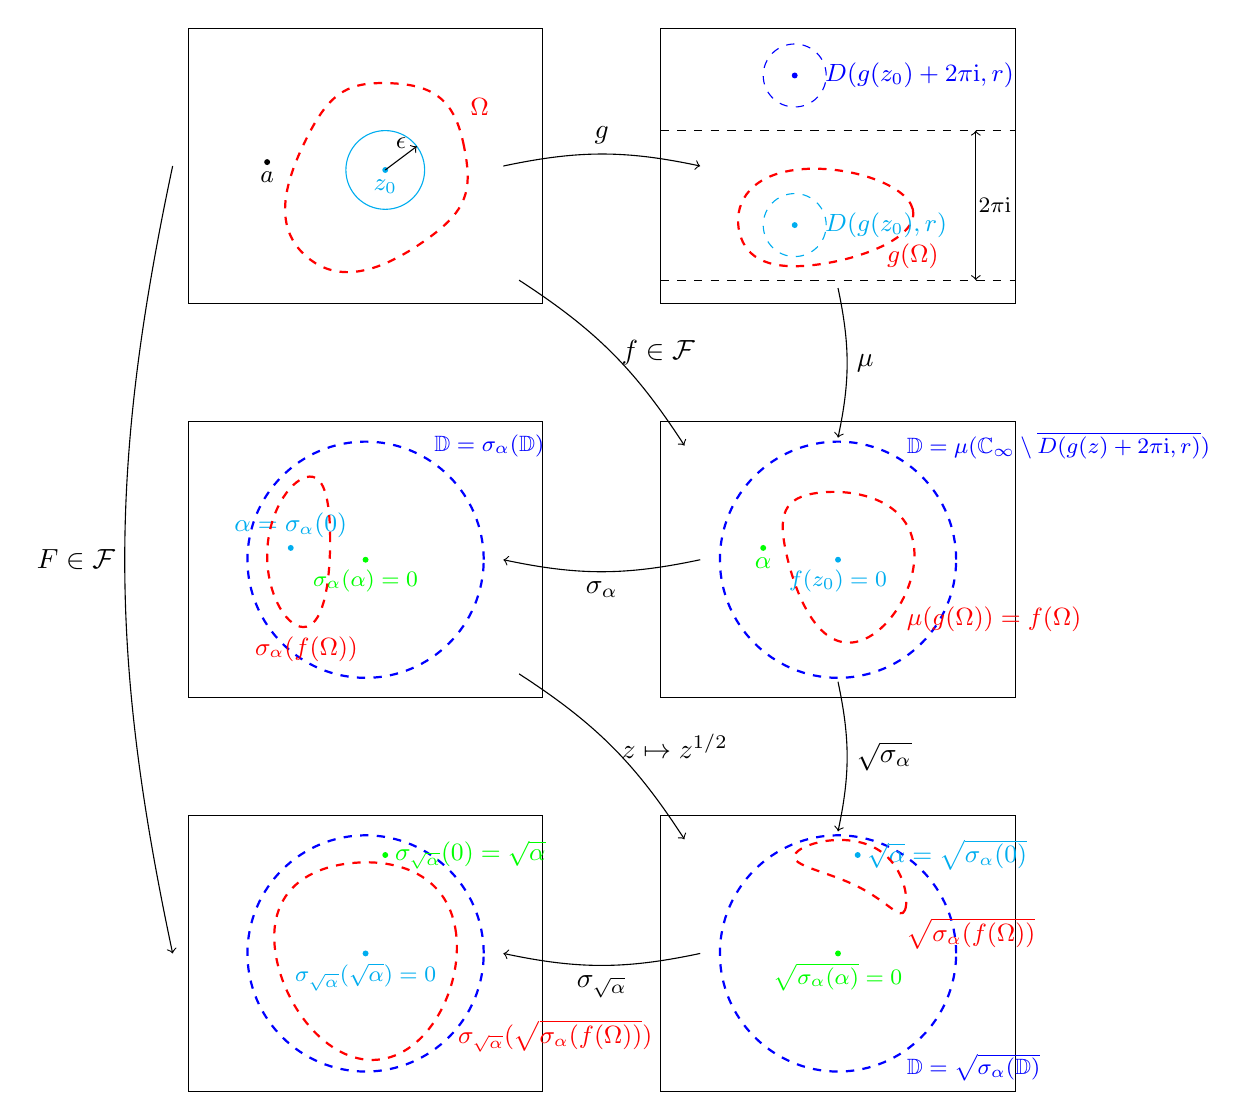
\begin{tikzpicture}
                    \draw (0,0) rectangle (4.5,3.5);
                    \draw[fill=black] (1,1.8) circle (0.03) node[below]{\small \(a\)};
                    \draw[red,dashed,thick] plot[smooth cycle, tension=1] coordinates {(3,0.8) (3.5,2) (2.6,2.8) (1.5,2.1) (1.5,0.6) };
                    \node[red] at (3.7,2.5) {\small \(\Omega\)};
                    \draw[cyan,fill=cyan] (2.5,1.7) circle (0.03) node[below] {\small \(z_0\)};
                    \draw[cyan] (2.5,1.7) circle (0.5);
                    \draw[->] (2.5,1.7)--node[above]{\small\(\epsilon\)}(2.9,2);

                    \draw[->] (4,1.75) to [bend left=12] node[above]{\(g\)}(6.5,1.75);
                    
                    \draw (6,0) rectangle (10.5,3.5);
                    \draw[dashed] (6,0.3)--(10.5,0.3);
                    \draw[dashed] (6,2.2)--(10.5,2.2);
                    \draw[<->] (10,0.3)--node[right=-0.25em]{\footnotesize\(2\pi \ii\)}(10,2.2);
                    \draw[red,dashed,thick] plot[smooth cycle, tension=1] coordinates {(8,0.5) (9.2,1.2) (7.7,1.7) (7,0.9) };
                    \node[red] at (9.2,0.6) {\small \(g(\Omega)\)};
                    \draw[cyan,fill=cyan] (7.7,1) circle (0.03) node[right=0.75em]{\small \(D(g(z_0),r)\)};
                    \draw[blue,fill=blue] (7.7,2.9) circle (0.03) node[right=0.75em]{\small \(D(g(z_0)+2\pi \ii,r)\)};
                    \draw[dashed,cyan] (7.7,1) circle (0.4);
                    \draw[dashed,blue] (7.7,2.9) circle (0.4);
                    
                    \draw[->] (8.25,0.2) to [bend left=12] node[right]{\(\mu\)}(8.25,-1.7);
                    \draw[->] (4.2,0.3) to [bend left=12] node[right]{\(f\in\mathcal{F}\)}(6.3,-1.8);
                    \draw[->] (6.5,-3.25) to [bend left=12] node[below]{\(\sigma_\alpha\)}(4,-3.25);
                    
                    \draw (0,-5) rectangle (4.5,-1.5);
                    \draw[green,fill=green] (2.25,-3.25) circle (0.03) node[below]{\footnotesize\(\sigma_\alpha(\alpha)=0\)};
                    \draw[dashed, thick, blue] (2.25,-3.25) circle (1.5);
                    \node[blue] at (3,-1.8)[right] {\footnotesize\(\DD=\sigma_\alpha(\DD)\)};
                    \draw[cyan,fill=cyan] (1.3,-3.1)circle(0.03)node[above]{\small\(\alpha=\sigma_\alpha(0)\)}; 
                    \draw[red,dashed,thick] plot[smooth cycle, tension=1] coordinates {(1.5,-4.1) (1.8,-3) (1.5,-2.2) (1,-3.2)};
                    \node[red] at (1.5,-4.1)[below]{\small\(\sigma_\alpha(f(\Omega))\)};

                    \draw (6,-5) rectangle (10.5,-1.5);
                    \draw[cyan,fill=cyan] (8.25,-3.25) circle (0.03) node[below]{\footnotesize\(f(z_0)=0\)};
                    \draw[dashed, thick, blue] (8.25,-3.25) circle (1.5);
                    \node[blue] at (9,-1.8)[right] {\footnotesize\(\DD=\mu(\CC_\infty\setminus\overline{D(g(z)+2\pi \ii,r)})\)};
                    \draw[red,dashed,thick] plot[smooth cycle, tension=1] coordinates {(8.44,-4.3) (9.2,-3) (8,-2.4) (7.6,-3.2)};
                    \node[red] at (9,-4)[right]{\small \(\mu(g(\Omega))=f(\Omega)\)};
                    \draw[green,fill=green] (7.3,-3.1)circle(0.03)node[below]{\small\(\alpha\)};
                    
                    \draw[->] (8.25,-4.8) to [bend left=12] node[right]{\(\sqrt{\sigma_\alpha}\)}(8.25,-6.7);
                    \draw[->] (4.2,-4.7) to [bend left=12] node[right]{\(z\mapsto z^{1/2}\)}(6.3,-6.8);
                    \draw[->] (6.5,-8.25) to [bend left=12] node[below]{\(\sigma_{\sqrt{\alpha}}\)}(4,-8.25);
                    \draw[->] (-0.2,1.75) to [bend right=12] node[left]{\(F\in\mathcal{F}\)}(-0.2,-8.25);

                    \draw (0,-10) rectangle (4.5,-6.5);
                    \draw[cyan,fill=cyan] (2.25,-8.25) circle (0.03) node[below]{\footnotesize\(\sigma_{\sqrt{\alpha}}(\sqrt{\alpha})=0\)};
                    \draw[dashed, thick, blue] (2.25,-8.25) circle (1.5);
                    \draw[green,fill=green] (2.5,-7)circle(0.03)node[right]{\small\(\sigma_{\sqrt{\alpha}}(0)=\sqrt{\alpha}\)};
                    \draw[red,dashed,thick] plot[smooth cycle, tension=1] coordinates {(2.4,-9.6) (3.4,-8) (2.1,-7.1) (1.1,-8.2)};
                    \node[red] at (3.3,-9.3)[right]{\small\(\sigma_{\sqrt{\alpha}}(\sqrt{\sigma_\alpha(f(\Omega))})\)};

                    \draw (6,-10) rectangle (10.5,-6.5);
                    \draw[green,fill=green] (8.25,-8.25) circle (0.03) node[below]{\footnotesize\(\sqrt{\sigma_\alpha(\alpha)}=0\)};
                    \draw[dashed, thick, blue] (8.25,-8.25) circle (1.5);
                    \node[blue] at (9,-9.7)[right] {\footnotesize\(\DD=\sqrt{\sigma_\alpha(\DD)}\)};
                    \draw[cyan,fill=cyan] (8.5,-7)circle(0.03)node[right]{\small\(\sqrt{\alpha}=\sqrt{\sigma_\alpha(0)}\)}; 
                    \draw[red,dashed,thick] plot[smooth cycle, tension=1] coordinates {(8.5,-7.4) (9.1,-7.7) (8.7,-6.9) (7.7,-7)};
                    \node[red] at (9,-8)[right]{\small\(\sqrt{\sigma_\alpha(f(\Omega))}\)};
                \end{tikzpicture}
            \end{figure}

            \begin{enumerate}[topsep=0pt]
                \item Consider simply connected domain \(\Omega\subsetneq\CC\), then \(\exists a\in\CC\setminus\Omega\). By example sheet 2, \(\exists\) holomorphic branch of \(\log(z-a)\) on \(\Omega\). Call it \(g(z)\). Since \(\ee^{g(z)}=z-a\), \(g\) has a well defined inverse on \(g(\Omega)\), so it is injective. Consider \(g(w)=g(z_0)+2\pi \ii\), then \(w-z_0=\ee^{g(w)}-\ee^{g(z_0)}=0\). A contradiction for \(g\) being injective no point in \(g\) can be mapped to \(g(z_0)+2\pi \ii\). Therefore by the open mapping theorem, \(\exists r>0\) such that \(D(g(z_0),r)\subset g(\Omega)\) while \(D(g(z_0)+2\pi \ii,r)\cap g(\Omega)=\varnothing\). Let \(\mu\) be the M\"{o}bius map sending \(\CC_{\infty}\setminus\overline{D(g(z_0)+2\pi \ii,\gamma)}\) to \(\DD\) and \(g(z_0)\) to \(0\). Then \(\mu\circ g\in\mathcal{F}\) so \(\mathcal{F}\ne\varnothing\).
                \item By Cauchy integral formula, for any \(f\in\mathcal{F}\), we have
                \[f'(z_0)=\frac{1}{2\pi \ii}\int_{C(z_0,\epsilon)}\frac{f(\zeta)}{(\zeta-z_0)^2}\dd{\zeta}\,,\]
                where \(\epsilon\) is chosen such that \(\overline{D(z_0,\epsilon)}\subseteq\Omega\). So
                \[\abs{f'(z_0)}\le\frac{1}{2\pi}\cdot 2\pi\epsilon\cdot1\cdot\frac{1}{\epsilon^2}=\frac{1}{\epsilon\,,}\]
                so \(m=\sup_{f\in\mathcal{F}}\abs{f'(z_0)}\) is finite and positive. Take a sequence \(\{f_n\}\subseteq\mathcal{F}\) such that \(\abs{f_n'(z_0)}\to m\). Since \(f(\Omega)\subseteq\DD\) \(\forall f\in\mathcal{F}\), \(\mathcal{F}\) is a normal family by Montel's theorem, so \(\exists\) subsequence \(\{f_{n_k}\}\) which converges locally uniformly to some holomorphic \(f\) on \(\Omega\). We have \(\abs{f'(z_0)}=m>0\) so \(f\) is non-constant, so it must be injective with \(f(\Omega)\subseteq\overline{\DD}\). By open mapping theorem, \(f(\Omega)\subseteq\inter(\overline{\DD})=\DD\), so \(f\in\mathcal{F}\).
                \item Claim that such \(f\) with maximum \(\abs{f'(z_0)}\) is surjective. If not, then \(\exists \alpha\in\DD\setminus f(\Omega)\). Consider the M\"{o}bius map
                \[\sigma_{\alpha}(z)=\frac{z-\alpha}{\overline{\alpha}z-1}\,.\]
                It is easy to check that it maps 0 to \(\alpha\), \(\alpha\) to zero and \(\DD\) to \(\DD\) itself. Hence \(\sigma_\alpha\circ f(\Omega)\) is a simply connected subset of \(\DD^\times\). Therefore \(\exists\) a holomorphic branch of \(\log\) on \(\sigma_\alpha\circ f(\Omega)\), and in particular, there \(\exists\) a holomorphic branch of \(z\mapsto z^{1/2}\). Call this square root map \(s\). Then the map
                \[s\circ\sigma_{\alpha}\equiv\sqrt{\sigma_\alpha}\]
                maps \(\alpha\) to 0, 0 to \(\sqrt{\alpha}\) and \(\DD\) to \(\DD\). Now consider \(\sigma_{\sqrt{\alpha}}\). It will take 0 to \(\sqrt{\alpha}\), \(\sqrt{\alpha}\) to zero and \(\DD\) to \(\DD\) itself again. Then we define
                \[F=\sigma_{s(\alpha)}\circ s\circ\sigma_{\alpha}f\,,\]
                which, from our discussion above, is clearly holomorphic, injective and \(F(z_0)=0\). Therefore we have found another \(F\in\mathcal{F}\). We want to show that it has larger derivative at \(z_0\) than \(f\) which contradicts our assumption. Denote \(h\) the squaring map and
                \[\Phi=\sigma_{\alpha}^{-1}\circ h\circ\sigma_{s(\alpha)}^{-1}:\DD\to\DD\]
                holomorphic, then \(f=\Phi F\). Since \(\Phi\) is not injective, it is not a rotation, and so \(\abs{\Phi'(0)}<1\) by Schwarz's lemma. Then by chain rule,
                \[\abs{f'(z_0)}=\abs{\Phi'(0)}\abs{F'(z_0)}<\abs{F'(z_0)}\]
                so contradiction.
            \end{enumerate}\qed
        \end{proof}
        \begin{rem}
            This can be further generalised to give the uniformisation theorem, which states that every simply connected Riemann surface is conformally equivalent to one of three Riemann surfaces: the open unit disk, the complex plane, or the Riemann sphere.
        \end{rem}
    \end{app}
    \begin{app}
        \textbf{(Newton's method in complex dynamics)}

        Recall the iterative root-finding algorithm that takes a polynomial \(p(z)\) and an initial guess \(z_0\) for a root of \(p\) and compute
        \[z_n=z_{n-1}-\frac{p(z_{n-1})}{p'(z_{n-1})}\,,\]
        and hope that \(z_n\to\) a root of \(p\). Hence, finding the roots of \(p\) is equivalent to finding the fixed point of
        \[f(z)=z-\frac{p(z)}{p'(z)}\,.\]

        For example, if we want to find the roots of \(p(z)=z^3-1\), we can turn to determine the fixed points of 
        \[f(z)=z-\frac{z^3-1}{3z^2}=\frac{2z^3+1}{3z^2}\,.\]
        \begin{figure}[ht!]
            \centering
            \begin{tikzpicture}
                \draw[->] (-2,0)--(2,0);
                \draw[->] (0,-2)--(0,2);
                \draw[domain=0.35:2.67, smooth, variable=\x] plot ({\x/1.5}, {(2*(\x^3)+1)/(4.5*(\x^2))});
                \draw[domain=-2.67:-0.32, smooth, variable=\x] plot ({\x/1.5}, {(2*(\x^3)+1)/(4.5*\x*\x)});
                \draw[dashed] (-2,-2)--(2,2);
            \end{tikzpicture}
        \end{figure}

        We can define the family \(\mathcal{F}=\{f^{\circ n}=\underbrace{f\circ\dots\circ f}_{n\text{ times}}\mid n\in\NN\}\) of meromorphic functions, and we want to know if their values approach a limit at \(z_0\).

        \begin{defn}
            The \textit{Fatou set} of a meromorphic \(f:\CC_\infty\to\CC_{\infty}\) is
            \[F(f)\coloneqq\{z\in C_\infty\mid\exists\text{ neighbourhood }U\text{ of }z_0\text{ on which }\{f^{\circ n}\}\text{ forms a normal family}\}\,.\]
            The \textit{Julia set} is the complement of the Fatou set
            \[J(f)\coloneqq\CC_\infty\setminus F(f)\,.\]
        \end{defn}

        \begin{figure}[ht!]
            \centering
            \begin{tikzpicture}
                \node at (0,0) {\includegraphics[width=0.8\textwidth]{Fatou.png}};
                \draw[fill=black] (1.35,0) circle (0.03) node [below]{\(z_1=1\)};
                \draw[fill=black] (-0.68,1.16) circle (0.03) node [below]{\(z_2=\omega\)};
                \draw[fill=black] (-0.68,-1.16) circle (0.03) node [below]{\(z_3=\omega^2\)};
                \node at (4,0.35) {points};
                \node at (4,0) {converging};
                \node at (4,-0.35) {to \(z_1\)};
                \node at (-2.5,2.35) {points};
                \node at (-2.5,2) {converging};
                \node at (-2.5,1.65) {to \(z_2\)};
                \node at (-2.5,-1.65) {points};
                \node at (-2.5,-2) {converging};
                \node at (-2.5,-2.35) {to \(z_3\)};
            \end{tikzpicture}
            \caption{Newton method for \(p(z)=z^3-1\), \(f(z)=\frac{2z^3+1}{3z^2}\), Fatou sets \(F(f)\) in colours. The brightness of the colour shows the speed of convergence.}
        \end{figure}
        \begin{ex}
            The Fatou set for \(f(z)=z^k\), \(k>1\) is \(F(f)=\DD\cup(\CC_\infty\setminus\overline{D})\). Since \(f^{\circ n}(z)=z^{k^n}\), if \(z\in\partial \DD\), and \(U\) is a neighbourhood of \(z\) with \(f^{\circ n}(z)\to f(z)\) as a holomorphic limit, then \(f|_{U\cap\DD}\equiv 0\) but \(f|_{U\cap(\CC_\infty\setminus\overline{D})}\equiv\infty\). Contradiction.
        \end{ex}
    \end{app}



    















\end{document}